% =====================================================================
%  EdgeGuard: Integrity Attestation and Layerwise Intrusion Detection
%  for Quantized Neural Networks on Edge Accelerators
%
%  M.Tech Project Report -- CS24M513, IIT Madras, 2026
%  Prepared with AI assistance (Claude, Anthropic) -- see the
%  "Statement on the Use of AI Tools" in the front matter.
%
%  Build:  cd report/thesis && latexmk -pdf main.tex
%  All experimental numbers are \input from ../generated/, which is
%  produced by experiments/make_tables.py from experiments/results/.
% =====================================================================
\documentclass[12pt,a4paper,oneside]{report}

\usepackage[a4paper,top=1in,bottom=1in,left=1.25in,right=1in]{geometry}
\usepackage[T1]{fontenc}
\usepackage{mathptmx}
\renewcommand{\ttdefault}{lmtt}
\usepackage{setspace}
\usepackage{amsmath,amssymb,amsthm}
\usepackage{graphicx}
\usepackage{booktabs,longtable,array,multirow,tabularx}
\usepackage{enumitem}
\usepackage{algorithm}
\usepackage{algpseudocode}
\usepackage{listings}
\usepackage{xcolor}
\usepackage{caption}
\usepackage{subcaption}
\usepackage{tikz}
\usetikzlibrary{arrows.meta,positioning,shapes.geometric,shapes.misc,fit,backgrounds,calc,decorations.pathreplacing}
\usepackage{fancyhdr}
\usepackage{titlesec}
\usepackage{tocloft}
\usepackage{pifont}
\usepackage{url}
\usepackage[hidelinks]{hyperref}
\usepackage[nameinlink,noabbrev]{cleveref}

\onehalfspacing
\setlength{\parskip}{0.35em}
\graphicspath{{../figures/}}

% ---- colours used in diagrams (validated categorical slots 1-3) -------
\definecolor{egblue}{HTML}{257DE0}
\definecolor{egorange}{HTML}{F47230}
\definecolor{egaqua}{HTML}{00B894}
\definecolor{egink}{HTML}{191919}
\definecolor{eggray}{HTML}{666666}
\definecolor{eglight}{HTML}{EEF4FC}

% ---- headers -----------------------------------------------------------
\pagestyle{fancy}
\fancyhf{}
\fancyhead[L]{\small\nouppercase{\leftmark}}
\fancyhead[R]{\small EdgeGuard}
\fancyfoot[C]{\thepage}
\renewcommand{\headrulewidth}{0.4pt}
\fancypagestyle{plain}{\fancyhf{}\fancyfoot[C]{\thepage}\renewcommand{\headrulewidth}{0pt}}

\titleformat{\chapter}[display]{\normalfont\huge\bfseries}{\chaptertitlename\ \thechapter}{12pt}{\Huge}
\titlespacing*{\chapter}{0pt}{-10pt}{30pt}

% ---- code listings -----------------------------------------------------
\lstdefinestyle{eg}{
  basicstyle=\ttfamily\footnotesize, keywordstyle=\color{egblue}\bfseries,
  commentstyle=\color{eggray}\itshape, stringstyle=\color{egorange!80!black},
  breaklines=true, frame=lines, framesep=4pt, numbers=left, numberstyle=\tiny\color{eggray},
  xleftmargin=1.5em, tabsize=4, showstringspaces=false, columns=fullflexible, keepspaces=true}
\lstset{style=eg,language=Python,
  literate={—}{{---}}1 {→}{{$\to$}}1 {✓}{{\checkmark}}1 {•}{{$\bullet$}}1}

% ---- theorem environments ---------------------------------------------
\theoremstyle{definition}
\newtheorem{definition}{Definition}[chapter]
\newtheorem{assumption}{Assumption}[chapter]
\theoremstyle{plain}
\newtheorem{proposition}{Proposition}[chapter]
\newtheorem{lemma}[proposition]{Lemma}
\theoremstyle{remark}
\newtheorem{remark}{Remark}[chapter]

% ---- macros --------------------------------------------------------------
\newcommand{\R}{\mathbb{R}}
\newcommand{\Z}{\mathbb{Z}}
\newcommand{\E}{\mathbb{E}}
\newcommand{\cmark}{\ding{51}}
\newcommand{\xmark}{\ding{55}}
\newcommand{\pmark}{$\circ$}
\newcommand{\code}[1]{\texttt{#1}}
\newcommand{\Hash}{\mathrm{H}}
\DeclareMathOperator{\clamp}{clamp}
\DeclareMathOperator{\round}{round}

% AUTO-GENERATED by experiments/make_tables.py -- do not edit
\newcommand{\NSeeds}{5}
\newcommand{\NPerSeed}{200}
\newcommand{\NPerScenario}{1000}
\newcommand{\NCalib}{500}
\newcommand{\ActDim}{32}
\newcommand{\TinyLayers}{39}
\newcommand{\TinyParams}{366{,}144}
\newcommand{\MChannels}{1{,}248}
\newcommand{\PSingleZFour}{6.33\times 10^{-5}}
\newcommand{\PredFPRZFour}{7.6\%}
\newcommand{\EmpFPRZFour}{7.2\%}
\newcommand{\ZBonf}{4.46}
\newcommand{\EmpFPRBonf}{0.9\%}
\newcommand{\ExpMaxGauss}{3.35}
\newcommand{\CleanMaxZMean}{3.48}
\newcommand{\CleanMaxZPNinetyNine}{4.45}
\newcommand{\SynergyTPRBonf}{0.4\%}
\newcommand{\PyVer}{3.13.18}
\newcommand{\NpVer}{2.5.3}
\newcommand{\CPUCount}{2}
\newcommand{\WallTime}{45}
\newcommand{\AUCSynergy}{0.64}
\newcommand{\FlagClean}{7.2\%}
\newcommand{\TypeClean}{92.8\%}
\newcommand{\MonClean}{7.2\%}
\newcommand{\LatClean}{1.57}
\newcommand{\LatPClean}{3.36}
\newcommand{\AttClean}{0.51}
\newcommand{\MonMsClean}{0.37}
\newcommand{\FlagBfaRandom}{100.0\%}
\newcommand{\TypeBfaRandom}{100.0\%}
\newcommand{\MonBfaRandom}{7.9\%}
\newcommand{\LatBfaRandom}{1.61}
\newcommand{\LatPBfaRandom}{3.11}
\newcommand{\AttBfaRandom}{0.52}
\newcommand{\MonMsBfaRandom}{0.35}
\newcommand{\FlagBfaSignBit}{100.0\%}
\newcommand{\TypeBfaSignBit}{100.0\%}
\newcommand{\MonBfaSignBit}{7.7\%}
\newcommand{\LatBfaSignBit}{1.52}
\newcommand{\LatPBfaSignBit}{2.53}
\newcommand{\AttBfaSignBit}{0.48}
\newcommand{\MonMsBfaSignBit}{0.33}
\newcommand{\FlagBfaProgressive}{100.0\%}
\newcommand{\TypeBfaProgressive}{100.0\%}
\newcommand{\MonBfaProgressive}{7.7\%}
\newcommand{\LatBfaProgressive}{1.59}
\newcommand{\LatPBfaProgressive}{2.60}
\newcommand{\AttBfaProgressive}{0.50}
\newcommand{\MonMsBfaProgressive}{0.35}
\newcommand{\FlagSupplySteg}{100.0\%}
\newcommand{\TypeSupplySteg}{0.0\%}
\newcommand{\MonSupplySteg}{6.9\%}
\newcommand{\LatSupplySteg}{1.60}
\newcommand{\LatPSupplySteg}{2.99}
\newcommand{\AttSupplySteg}{0.50}
\newcommand{\MonMsSupplySteg}{0.36}
\newcommand{\FlagSupplyDistributed}{100.0\%}
\newcommand{\TypeSupplyDistributed}{100.0\%}
\newcommand{\MonSupplyDistributed}{7.3\%}
\newcommand{\LatSupplyDistributed}{1.63}
\newcommand{\LatPSupplyDistributed}{2.84}
\newcommand{\AttSupplyDistributed}{0.51}
\newcommand{\MonMsSupplyDistributed}{0.36}
\newcommand{\FlagAdvTextInjection}{100.0\%}
\newcommand{\TypeAdvTextInjection}{100.0\%}
\newcommand{\MonAdvTextInjection}{100.0\%}
\newcommand{\LatAdvTextInjection}{1.60}
\newcommand{\LatPAdvTextInjection}{2.68}
\newcommand{\AttAdvTextInjection}{0.49}
\newcommand{\MonMsAdvTextInjection}{0.38}
\newcommand{\FlagAdvSafetyBypass}{100.0\%}
\newcommand{\TypeAdvSafetyBypass}{0.0\%}
\newcommand{\MonAdvSafetyBypass}{100.0\%}
\newcommand{\LatAdvSafetyBypass}{1.61}
\newcommand{\LatPAdvSafetyBypass}{2.55}
\newcommand{\AttAdvSafetyBypass}{0.50}
\newcommand{\MonMsAdvSafetyBypass}{0.37}
\newcommand{\FlagExfilProbe}{100.0\%}
\newcommand{\TypeExfilProbe}{100.0\%}
\newcommand{\MonExfilProbe}{100.0\%}
\newcommand{\LatExfilProbe}{1.68}
\newcommand{\LatPExfilProbe}{3.79}
\newcommand{\AttExfilProbe}{0.52}
\newcommand{\MonMsExfilProbe}{0.39}
\newcommand{\FlagSynergy}{100.0\%}
\newcommand{\TypeSynergy}{100.0\%}
\newcommand{\MonSynergy}{4.7\%}
\newcommand{\LatSynergy}{1.54}
\newcommand{\LatPSynergy}{3.29}
\newcommand{\AttSynergy}{0.51}
\newcommand{\MonMsSynergy}{0.34}
\newcommand{\LatMin}{1.52}
\newcommand{\LatMax}{1.68}
\newcommand{\LatPMax}{3.8}
\newcommand{\MerkThrMin}{888}
\newcommand{\MerkThrMax}{1039}
\newcommand{\SafetyAdvFrac}{32.9\%}
\newcommand{\SafetyTFFrac}{67.1\%}
\newcommand{\CleanAdvFrac}{2.9\%}
\newcommand{\CleanTFFrac}{4.3\%}
\newcommand{\MerkVerTinyllm}{0.4}
\newcommand{\MerkSizeTinyllm}{0.3}
\newcommand{\MerkThrTinyllm}{786}
\newcommand{\MerkVerQwenPPB}{575.6}
\newcommand{\MerkSizeQwenPPB}{598.3}
\newcommand{\MerkThrQwenPPB}{1039}
\newcommand{\MerkVerLlamaPB}{1578.3}
\newcommand{\MerkSizeLlamaPB}{1401.1}
\newcommand{\MerkThrLlamaPB}{888}
\newcommand{\FidMemoryDump}{1.00000}
\newcommand{\FidColdBoot}{0.98772}
\newcommand{\FidEmSideChannel}{0.99999}
\newcommand{\NTests}{117}


% =====================================================================
\begin{document}

\pagenumbering{roman}
% ---------------------------------------------------------------- title
\begin{titlepage}
\begin{center}
\vspace*{0cm}
{\LARGE\bfseries EdgeGuard: Integrity Attestation and\\[0.2cm]
Layerwise Intrusion Detection for\\[0.2cm]
Quantized Neural Networks on Edge Accelerators\par}
\vspace{1.0cm}
{\large A Project Report\\[0.2cm] submitted in partial fulfilment of the requirements\\
for the award of the degree of\par}
\vspace{0.6cm}
{\Large\bfseries Master of Technology\par}
\vspace{0.3cm}
{\large in\\[0.2cm] Computer Science and Engineering\par}
\vspace{0.9cm}
{\large by\par}
\vspace{0.3cm}
{\Large\bfseries Arnav Deshpande\par}
{\large (CS24M513)\par}
\vspace{0.5cm}
{\normalsize Prepared with AI assistance from Claude (Anthropic);\\
see the Statement on the Use of AI Tools.\par}
\vfill
{\large\bfseries Department of Computer Science and Engineering\\[0.15cm]
Indian Institute of Technology Madras\\[0.15cm]
Chennai 600\,036\par}
\vspace{0.4cm}
{\large November 2026\par}
\end{center}
\end{titlepage}

% ---------------------------------------------------------------- certificate
\chapter*{Certificate}
\addcontentsline{toc}{chapter}{Certificate}
This is to certify that the report titled \textbf{EdgeGuard: Integrity Attestation and Layerwise
Intrusion Detection for Quantized Neural Networks on Edge Accelerators}, submitted by
\textbf{Arnav Deshpande (CS24M513)} to the Indian Institute of Technology Madras in partial
fulfilment of the requirements for the award of the degree of Master of Technology, is a
record of the project work carried out under my supervision.

\vspace{3cm}
\noindent
\begin{tabular}{@{}l@{\hspace{5cm}}l}
\rule{5cm}{0.4pt} & \\
\textbf{[Name of Guide]} & Place: Chennai \\
Project Guide & Date: \\
Department of Computer Science and Engineering & \\
IIT Madras &
\end{tabular}

% ---------------------------------------------------------------- AI statement
\chapter*{Statement on the Use of AI Tools}
\addcontentsline{toc}{chapter}{Statement on the Use of AI Tools}
This project was carried out with substantial assistance from Claude, a large language model
developed by Anthropic, which is credited as a co-author on the commits in the project
repository (\url{https://github.com/arnavd2001/edgeguard}). The assistance covered:

\begin{itemize}[leftmargin=*]
  \item drafting and debugging the Python implementation of the \textsc{EdgeGuard} framework,
        the attack simulators and the test suite;
  \item designing and running the experiments reported in \cref{ch:evaluation}, and generating
        the figures and tables from the recorded results;
  \item drafting the text of this report.
\end{itemize}

\noindent
Every experimental number in this report is produced by the scripts in
\code{experiments/} and is inserted into the document automatically from
\code{experiments/results/results.json}; no result was typed by hand. Every bibliographic
reference was checked against the publisher's page, the arXiv listing or a bibliographic
database (DBLP, Crossref, PMLR, ACL Anthology). An earlier draft of this report contained
results that had not been measured and references that could not be verified; those were
removed, and the corresponding sections were rewritten from measured data.

\noindent
The candidate is responsible for the content of this report, has reviewed it, and should be
able to explain every design decision and result in it.

\vspace{1.5cm}
\noindent Arnav Deshpande \hfill Date: \underline{\hspace{3cm}}

% ---------------------------------------------------------------- acknowledgements
\chapter*{Acknowledgements}
\addcontentsline{toc}{chapter}{Acknowledgements}
\textit{[To be written by the candidate.]}

% ---------------------------------------------------------------- abstract
\chapter*{Abstract}
\addcontentsline{toc}{chapter}{Abstract}

Neural networks deployed on edge accelerators are stored and executed as 8-bit integer (INT8)
tensors in memory that an attacker may be able to read or corrupt. Three families of attack
are well documented: bit flips induced in DRAM that destroy or hijack a model, adversarial
inputs that steer it, and extraction of weights or memorised training data from it. Defences
in the literature usually address one family at a time. This report describes
\textsc{EdgeGuard}, a Python framework that combines two independent checks and a rule-based
classifier that labels what it sees.

The first check is a Merkle tree of SHA-256 digests over the model's weight tensors, with an
ECDSA P-256 signature on the root. It detects any change to the stored weights and names the
tensor that changed. The second check is a per-layer activation monitor calibrated with
Welford's streaming algorithm directly on INT8 activations, scoring each inference with a
channel-wise $z$-score and a Mahalanobis distance. A classifier maps the joint outcome to one of
eight reachable threat labels and emits a layer-by-layer explanation. The framework includes
simulators for bit-flip, supply-chain, adversarial-input, training-data-extraction and combined
(``synergy'') attacks, and a generator of INT8 weight sets shaped like five open-weight
language models.

Evaluation is carried out on simulated activations, with \NPerScenario{} inputs per scenario
across \NSeeds{} seeds. The Merkle check flagged every weight-modifying input in every scenario
and localised the modified tensor exactly in every case. The activation monitor alone flagged
only \MonSynergy{} of synergy inputs, which perturb weights and suppress the activation signal,
so the combined pipeline catches inputs that activation monitoring alone misses. A fixed
$4\sigma$ threshold produced a \EmpFPRZFour{} false-positive rate on clean inputs, which matches
the \PredFPRZFour{} predicted by a multiple-comparisons argument over \MChannels{} monitored
channels; a Bonferroni-corrected threshold of $z^*=\ZBonf$ reduced it to \EmpFPRBonf{} while
still flagging all three activation-level attack scenarios. Re-hashing a 1.4\,GiB weight set took
\MerkVerLlamaPB{}\,ms on the test machine, which rules out full attestation on every inference
for language-model-sized weights and motivates the amortised schemes discussed in
\cref{ch:discussion}. Because the attack generators and the detector were written together,
the activation-level results measure the internal consistency of the simulation rather than
robustness to an adaptive attacker; this limitation and a plan to evaluate on real models on a
Qualcomm Hexagon NPU are set out in \cref{ch:conclusion}.

\vspace{0.5cm}
\noindent\textbf{Keywords:} edge AI security, quantized neural networks, bit-flip attacks,
Merkle trees, anomaly detection, Mahalanobis distance, training-data extraction, NPU.

% ---------------------------------------------------------------- lists
\cleardoublepage
\tableofcontents
\cleardoublepage
\listoffigures
\addcontentsline{toc}{chapter}{List of Figures}
\cleardoublepage
\listoftables
\addcontentsline{toc}{chapter}{List of Tables}

% ---------------------------------------------------------------- abbreviations
\chapter*{Abbreviations}
\addcontentsline{toc}{chapter}{Abbreviations}
\begin{tabular}{@{}p{2.6cm}p{11cm}@{}}
AUC   & Area under the (ROC) curve \\
BFA   & Bit-flip attack \\
CVD   & Colour-vision deficiency \\
DMA   & Direct memory access \\
DRAM  & Dynamic random-access memory \\
ECDSA & Elliptic Curve Digital Signature Algorithm \\
EM    & Electromagnetic (side channel) \\
FFN   & Feed-forward network (transformer MLP block) \\
FPR   & False-positive rate \\
FP32  & 32-bit IEEE-754 floating point \\
HTP   & Hexagon Tensor Processor \\
INT8  & 8-bit signed two's-complement integer \\
LLM   & Large language model \\
LSB / MSB & Least / most significant bit \\
NPU   & Neural processing unit \\
PBFA  & Progressive bit-flip attack \\
PTQ   & Post-training quantization \\
QAT   & Quantization-aware training \\
QNN   & Qualcomm AI Engine Direct SDK (``Qualcomm Neural Network'') \\
ROC   & Receiver operating characteristic \\
SHA-256 & Secure Hash Algorithm, 256-bit output \\
TEE   & Trusted execution environment \\
TOCTOU & Time of check to time of use \\
TPR   & True-positive rate \\
\end{tabular}

% ---------------------------------------------------------------- notation
\chapter*{Notation}
\addcontentsline{toc}{chapter}{Notation}
\begin{tabular}{@{}p{2.6cm}p{11cm}@{}}
$L_i$                     & $i$-th weight tensor of a model, $i = 0,\dots,n-1$ \\
$n$                       & number of weight tensors (Merkle leaves) \\
$\Hash(\cdot)$            & SHA-256 \\
$h_i$                     & leaf digest of $L_i$ \\
$r$                       & Merkle root \\
$\sigma$                  & ECDSA signature on $r$ \\
$\mathbf{a}_\ell\in\Z^{d}$ & INT8 activation vector at monitored layer $\ell$, dimension $d$ \\
$\boldsymbol\mu_\ell,\boldsymbol\sigma_\ell$ & per-channel calibration mean and standard deviation \\
$\hat\Sigma_\ell$         & calibration covariance; $\hat\Sigma_\ell^{+}$ its pseudo-inverse \\
$Z_\ell$                  & max channel $|z|$-score at layer $\ell$ \\
$D_\ell$                  & Mahalanobis distance at layer $\ell$ \\
$\tau_z,\tau_D$           & $z$-score and Mahalanobis thresholds \\
$m$                       & total monitored channels, $m=\sum_\ell d_\ell$ \\
$s, z_0$                  & quantization scale and zero point \\
\end{tabular}


\cleardoublepage
\pagenumbering{arabic}
\chapter{Introduction}
\label{ch:introduction}

\section{Motivation}

Inference on phones, vehicles and embedded controllers is now commonly carried out by a
dedicated neural processing unit (NPU) rather than by the application CPU. Qualcomm's
Snapdragon platforms, for example, expose a Hexagon NPU through the Qualcomm AI Engine Direct
SDK, which provides a unified low-level API across the CPU, GPU and NPU of the chip
\cite{qualcomm_qnn}. To fit such hardware, a model is first compressed. The most common
compression is post-training quantization to 8-bit integers (INT8), which cuts weight storage
to a quarter of its 32-bit floating-point (FP32) size and allows integer-only arithmetic
\cite{jacob2018quantization,nagel2021whitepaper}. For large language models (LLMs), techniques
such as GPTQ \cite{frantar2023gptq} and SmoothQuant \cite{xiao2023smoothquant} make 8-bit and
lower-precision inference practical at billion-parameter scale, and model families such as
Llama~3.2, Qwen2.5 and Phi-3.5 include sizes intended for on-device use
\cite{llama3herd,qwen25report,phi3report}.

The deployed artefact is therefore a set of INT8 tensors held in DRAM, read by an accelerator
through direct memory access, and executed by a vendor runtime. That artefact has three
security properties worth protecting.

\begin{description}[leftmargin=*,style=nextline]
  \item[Integrity of the weights.] Rowhammer, first shown by Kim et al.\ \cite{kim2014flipping},
        lets unprivileged code flip bits in neighbouring DRAM rows. Hong et al.\ showed that most
        of the 19 image models they studied contain at least one parameter whose single bit flip
        drops accuracy by more than 90\% \cite{hong2019terminal}. Rakin et al.'s progressive
        bit-flip attack (PBFA) searches for the most damaging bits in quantized models
        \cite{rakin2019bfa}, and DeepHammer carried out such an attack end to end on real
        hardware, degrading accuracy to random guessing within minutes \cite{yao2020deephammer}.
        Model weights can also be modified before they reach the device, in the model supply
        chain. Feng and Tram\`er showed that a tampered pretrained model can expose the data
        on which it is later fine-tuned \cite{feng2024privacy}.
  \item[Integrity of the computation's inputs.] Adversarial examples, small perturbations of
        an input chosen to change the output, are a long-established threat
        \cite{goodfellow2015explaining,madry2018towards}. For LLMs the corresponding threats
        include prompt injection and attempts to bypass safety training.
  \item[Confidentiality of the weights and the training data.] Weights can be stolen through
        a prediction API \cite{tramer2016stealing} or read physically. Cold-boot attacks recover
        DRAM contents after power loss \cite{halderman2008lest}. Once an attacker can query a
        model or holds its weights, memorised training data becomes a target. Carlini et al.\
        extracted verbatim training sequences, including personal information, from GPT-2
        \cite{carlini2021extracting}. Nasr et al.\ scaled such extraction to production models
        \cite{nasr2023scalable}. Dai et al.\ reconstructed training text from activations
        exchanged in decentralised training \cite{dai2025activation}.
\end{description}

Defences exist for each of these. For weight integrity there are checksum and hash
signatures over weights \cite{li2021radar,javaheripi2021hashtag,guo2021modelshield}, honeypot
neurons \cite{liu2023neuropots} and weight reconstruction \cite{li2020defending}. For inputs
there are feature-space detectors such as the Mahalanobis-distance detector of Lee et al.\
\cite{lee2018simple}. For confidentiality there are trusted-execution-environment (TEE) designs
such as Amulet \cite{mao2025amulet}. These defences are typically designed and evaluated in
isolation, and most image-model defences were not designed with transformer LLM weight layouts
in mind.

\section{The problem studied}

This project asks whether a single, lightweight runtime layer can provide three things together
for a quantized model on an edge accelerator:

\begin{enumerate}[label=(\roman*),leftmargin=*]
  \item a \emph{cryptographic} guarantee that the weights being executed are the weights that
        were signed at release, with the modified tensor identified when they are not;
  \item a \emph{statistical} check that each inference's internal activations are consistent
        with clean behaviour, computed on INT8 values without dequantizing;
  \item a \emph{label and explanation} for what was detected, so that an operator knows
        whether to reload weights, drop an input or investigate a probe.
\end{enumerate}

The motivating observation is that the two checks fail in complementary ways. A hash check
sees nothing wrong with an adversarial input, because the weights are unchanged. An activation
monitor can miss a weight attack if the attacker also controls the input and uses it to keep
activations looking normal. This combined attack is called a \emph{synergy attack} in this
report. It is a construction used for evaluation, not an attack taken from the literature.

\section{Research questions}

The work is organised around five questions. Each is answered, within the limits of a
simulation-based study, in \cref{ch:evaluation}.

\begin{description}[leftmargin=*,style=nextline]
  \item[RQ1 — Weight integrity.] Does per-tensor SHA-256 hashing organised as a signed Merkle
        tree detect every simulated weight modification, including single-bit and
        least-significant-bit changes, and does it identify the modified tensor?
  \item[RQ2 — Activation anomalies.] Does a monitor calibrated on INT8 activations separate the
        simulated adversarial and extraction-probe inputs from clean ones, and at what
        false-positive rate?
  \item[RQ3 — Complementarity.] Does combining the two checks catch inputs that either check
        alone would miss, in particular synergy inputs?
  \item[RQ4 — Labelling.] How often does the rule-based classifier assign the intended threat
        label, and where does it confuse classes?
  \item[RQ5 — Cost.] What does each check cost per inference, and how does attestation cost
        scale to weight sets of language-model size?
\end{description}

\section{Contributions}

The contributions of this phase of the project are stated below. The report is careful to
separate what was built and measured from what is planned.

\begin{enumerate}[leftmargin=*]
  \item \textbf{A combined attestation-and-monitoring framework.} \textsc{EdgeGuard} is an
        open-source Python package of about 4{,}000 lines (\cref{ch:implementation}). It
        provides a signed SHA-256 Merkle tree over weight tensors, an INT8 activation monitor
        built on Welford's streaming statistics \cite{welford1962note}, and a rule-based
        classifier that produces per-layer explanations. Hash-based weight checking is not new
        in itself \cite{javaheripi2021hashtag,guo2021modelshield}; the contribution is the
        integration with activation monitoring and threat labelling, and its application to
        transformer weight layouts.
  \item \textbf{A simulation testbed.} The package includes simulators for bit-flip attacks
        under four strategies, supply-chain poisoning under three, adversarial inputs under
        three, training-data-extraction probes, physical weight extraction under three channel
        models, and synergy attacks. It also includes a generator of INT8 weight sets with the
        tensor shapes and HuggingFace naming of five open-weight language models. A suite of
        \NTests{} automated tests covers the package.
  \item \textbf{A measured evaluation with an explained false-positive rate.} All numbers in
        \cref{ch:evaluation} are generated by a single script from recorded runs. The clean
        false-positive rate of a fixed $4\sigma$ threshold is shown to follow from a
        multiple-comparisons argument (predicted \PredFPRZFour{}, measured \EmpFPRZFour{}). A
        Bonferroni-corrected threshold brings it to \EmpFPRBonf{} without losing any of the
        activation-level detections.
  \item \textbf{Evidence for complementarity, and a cost limit.} In simulation, the activation
        monitor alone flagged \MonSynergy{} of synergy inputs while the combined pipeline
        flagged \FlagSynergy{}. Full re-attestation of a 1.4\,GiB weight set costs about 1.6\,s
        on the test machine, which bounds where per-inference attestation is practical.
  \item \textbf{Engineering findings.} Two defects in the initial attack simulators were found
        and fixed during the evaluation. Both were integer-overflow errors in the handling of
        two's-complement sign bits, and both are of a kind that would silently distort a
        bit-flip study (\cref{sec:impl:bugs}).
\end{enumerate}

\section{Scope and limitations}

Three limitations should be stated at the outset, because they qualify every result.

First, \textbf{no real model is executed}. The weight sets are random INT8 tensors with
realistic shapes. The activations are drawn from distributions defined in the attack
simulators, not produced by running a network. Weight-level results do not depend on this,
because a hash detects a changed byte regardless of what the byte means. Activation-level
results do depend on it.

Second, \textbf{the detector and the attack generators were written together}. An activation
detector that achieves an AUC of 1.0 against attacks whose activation distributions were chosen
by the same authors demonstrates that the pipeline works end to end. It does not demonstrate
robustness against an adaptive attacker. \Cref{ch:discussion} discusses this in detail.

Third, \textbf{no NPU measurements are reported}. The QNN adapter in the package is a
duck-typed interface that has been exercised only with test doubles. Latencies are measured on
a two-core x86 cloud machine and are reported as such.

\section{Organisation of the report}

\Cref{ch:background} covers the background needed for the rest of the report: quantization,
the NPU software stack, transformer weight layouts, the cryptographic primitives used, and the
statistics behind the monitor. \Cref{ch:related} reviews prior work on bit-flip attacks and
defences, input anomaly detection, model and data extraction, and supply-chain attacks.
\Cref{ch:threat} states the threat model. \Cref{ch:design} presents the design and argues the
properties of each component. \Cref{ch:implementation} describes the implementation, the
attack simulators and the test suite. \Cref{ch:evaluation} reports the experiments.
\Cref{ch:discussion} interprets them and discusses limitations. \Cref{ch:conclusion} concludes
and sets out the plan for the next phase. The appendices give the configuration file, the API
reference, the full test inventory, per-seed results and reproduction instructions.

\chapter{Background}
\label{ch:background}

This chapter collects the material that later chapters rely on. \Cref{sec:bg:quant} reviews
integer quantization and the effect of a single bit flip on an INT8 weight.
\Cref{sec:bg:npu} outlines the software stack through which a quantized model reaches a
Qualcomm NPU. \Cref{sec:bg:transformer} describes the weight layout of a decoder-only
transformer. \Cref{sec:bg:crypto} reviews the cryptographic primitives used for attestation,
and \cref{sec:bg:stats} the statistics used by the activation monitor.

% ---------------------------------------------------------------------------
\section{Integer quantization}
\label{sec:bg:quant}

\subsection{Affine and symmetric quantization}

Quantization maps a real-valued tensor $x$ to integers $q$ using a scale $s>0$ and a zero
point $z_0$ \cite{jacob2018quantization,nagel2021whitepaper}:
\begin{equation}
  q = \clamp\!\Big(\round\big(x/s\big) + z_0,\; q_{\min},\; q_{\max}\Big),
  \qquad \hat x = s\,(q - z_0).
  \label{eq:affine}
\end{equation}
For signed 8-bit storage, $q_{\min}=-128$ and $q_{\max}=127$. \emph{Symmetric} quantization
fixes $z_0=0$ and chooses $s = \max|x| / 127$, so that the largest-magnitude value maps to
$\pm127$. \emph{Asymmetric} quantization uses unsigned storage $[0,255]$ with
$s=(x_{\max}-x_{\min})/255$ and $z_0 = \round(-x_{\min}/s)$, which uses the full range
when the distribution is skewed. \textsc{EdgeGuard}'s helper \code{compute\_int8\_params}
implements both variants per tensor (\cref{ch:implementation}).

The reconstruction error of a value inside the clipping range is at most $s/2$. Rounding errors
are commonly modelled as uniform on $[-s/2,s/2]$ with variance $s^2/12$. This matters for the
monitor in two ways. Activations observed at runtime are integers, so their empirical variance
includes this quantization noise. And statistics computed in FP32 at calibration time and
compared against INT8 values at runtime would be measured in different units unless they are
rescaled. Calibrating directly on the INT8 values avoids this mismatch by construction.

\subsection{Per-tensor, per-channel and low-bit formats}

A single scale per tensor is simple but wastes resolution when channel magnitudes differ.
Per-channel quantization assigns a scale to each output channel of a weight matrix and is the
usual choice for convolution and linear weights \cite{nagel2021whitepaper}. Below eight bits,
formats such as INT4 pack two values per byte. \textsc{EdgeGuard} stores INT4 values in the
low and high nibbles of a byte and sign-extends them on unpacking. The attestation layer is
indifferent to these choices because it hashes the stored bytes, whatever they encode.

For LLMs, activation outliers make naive 8-bit activation quantization lossy. SmoothQuant
migrates part of the activation range into the weights with a mathematically equivalent
per-channel rescaling, enabling 8-bit weights and activations for models up to 530B parameters
\cite{xiao2023smoothquant}. GPTQ quantizes weights to 3--4 bits using approximate second-order
information \cite{frantar2023gptq}. Both produce integer tensors of the kind that
\textsc{EdgeGuard} attests.

\subsection{Two's complement and the cost of one bit}
\label{sec:bg:twos}

An INT8 value is stored as a byte $b_7b_6\dots b_0$ in two's complement:
\begin{equation}
  q = -128\,b_7 + \sum_{k=0}^{6} 2^k b_k .
\end{equation}
Flipping bit $k<7$ changes $q$ by exactly $\pm 2^k$. Flipping the sign bit $b_7$ changes $q$ by
$\pm128$ when interpreted in the signed range: for instance $-5$ (\code{0xFB}) becomes $123$
(\code{0x7B}), a change of $128$. In real units the change is $s\cdot 2^k$, so the
maximum single-flip perturbation of a weight is $128\,s$. \Cref{tab:bitflip_effect}
summarises the effect by bit position.

\begin{table}[t]
\centering
\caption{Effect of flipping one bit of an INT8 weight stored in two's complement.}
\label{tab:bitflip_effect}
\begin{tabular}{cccl}
\toprule
\textbf{Bit $k$} & \textbf{$|\Delta q|$} & \textbf{$|\Delta \hat x|$} & \textbf{Example ($q=-5$)} \\
\midrule
0 (LSB) & 1   & $s$     & $-5 \to -6$ \\
1       & 2   & $2s$    & $-5 \to -7$ \\
2       & 4   & $4s$    & $-5 \to -1$ \\
3       & 8   & $8s$    & $-5 \to -13$ \\
4       & 16  & $16s$   & $-5 \to -21$ \\
5       & 32  & $32s$   & $-5 \to -37$ \\
6       & 64  & $64s$   & $-5 \to -69$ \\
7 (sign)& 128 & $128s$  & $-5 \to 123$ \\
\bottomrule
\end{tabular}
\end{table}

A subtle implementation point follows from this arithmetic. In a high-level language, XORing a
\emph{signed} integer with $2^7$ does not reproduce the hardware effect. In Python,
\code{-5 \^{} 128} evaluates to $-133$, which is outside the INT8 range and either raises an
overflow error or, if clipped, saturates to $-128$ instead of wrapping to $123$. A faithful
simulator must operate on the unsigned byte view. Two such errors were found in the original
\textsc{EdgeGuard} simulators and are described in \cref{sec:impl:bugs}.

% ---------------------------------------------------------------------------
\section{The edge NPU software stack}
\label{sec:bg:npu}

\begin{figure}[t]
\centering
\begin{tikzpicture}[
  box/.style={draw=eggray, rounded corners=2pt, minimum width=10.5cm, minimum height=0.8cm,
              align=center, font=\small},
  hl/.style={box, fill=eglight, draw=egblue},
  node distance=0.18cm]
\node[box] (app) {Application (Android / Linux process)};
\node[box, below=of app] (fw) {Framework delegate: LiteRT, ONNX Runtime, ExecuTorch};
\node[hl, below=of fw] (qnn) {Qualcomm AI Engine Direct (QNN) API: backend, context, graph};
\node[box, below=of qnn, minimum width=3.3cm, xshift=-3.6cm] (cpu) {CPU backend};
\node[box, right=0.15cm of cpu, minimum width=3.3cm] (gpu) {GPU backend};
\node[box, right=0.15cm of gpu, minimum width=3.6cm, fill=eglight, draw=egblue] (htp) {HTP backend (NPU)};
\node[box, below=0.18cm of gpu, minimum width=10.5cm] (dram) {Shared DRAM: weights, activations, context binary};
\draw[-{Stealth}, eggray] (app) -- (fw);
\draw[-{Stealth}, eggray] (fw) -- (qnn);
\draw[-{Stealth}, eggray] (qnn.south) ++(-3.6,0) -- (cpu.north);
\draw[-{Stealth}, eggray] (qnn.south) -- (gpu.north);
\draw[-{Stealth}, eggray] (qnn.south) ++(3.45,0) -- (htp.north);
\node[right=0.3cm of dram, font=\scriptsize, text=egorange!80!black, align=left] {Rowhammer,\\cold boot};
\end{tikzpicture}
\caption{Simplified software stack for a quantized model on a Snapdragon device. The weights
that the NPU executes reside in DRAM shared with the rest of the system.}
\label{fig:npu_stack}
\end{figure}

Qualcomm's AI Engine Direct SDK, also referred to as QNN, provides a low-level API over the
Kryo CPU, Adreno GPU and Hexagon NPU, organised around tools, devices, backends, contexts,
graphs and an operation-package registry \cite{qualcomm_qnn}. Each processing unit is driven by a
\emph{backend} library; the HTP backend targets the Hexagon processor with its fused AI
accelerator \cite{qualcomm_qnn_backend}. Higher-level frameworks delegate to these backends.
ExecuTorch, for example, lowers PyTorch models to a QNN context binary for the HTP backend
\cite{executorch_qnn}.

Two properties of this stack matter here. First, the weights an NPU executes are stored in
system DRAM, which is shared with other software and exposed to DRAM-level attacks
(\cref{fig:npu_stack}). Second, the runtime is optimised for throughput and exposes inputs and
outputs, not intermediate activations, by default. Obtaining per-layer activations for
monitoring therefore requires either marking intermediate tensors as graph outputs at
compilation time or running an instrumented copy of the graph. \textsc{EdgeGuard}'s QNN adapter
is designed around the first option (\cref{sec:design:adapter}).

% ---------------------------------------------------------------------------
\section{Decoder-only transformer weight layout}
\label{sec:bg:transformer}

\begin{figure}[t]
\centering
\begin{tikzpicture}[
  w/.style={draw=egblue, fill=eglight, rounded corners=1.5pt, minimum height=0.55cm,
            font=\scriptsize\ttfamily, inner sep=2pt},
  n/.style={draw=eggray, rounded corners=1.5pt, minimum height=0.55cm, font=\scriptsize\ttfamily, inner sep=2pt},
  lab/.style={font=\scriptsize, text=eggray}]
\node[w, minimum width=4.2cm] (emb) at (0,0) {embed\_tokens  $V\times H$};
\begin{scope}[yshift=-1.0cm]
\node[n, minimum width=4.2cm] (ln1) at (0,0) {input\_layernorm  $H$};
\node[w, minimum width=2.0cm, anchor=north west] (q) at ($(ln1.south west)+(0,-0.15)$) {q\_proj $H\!\times\! H$};
\node[w, minimum width=2.0cm, anchor=north east] (k) at ($(ln1.south east)+(0,-0.15)$) {k\_proj $H\!\times\! d_h$};
\node[w, minimum width=2.0cm, anchor=north] (v) at ($(q.south)+(0,-0.15)$) {v\_proj $H\!\times\! d_h$};
\node[w, minimum width=2.0cm, anchor=north] (o) at ($(k.south)+(0,-0.15)$) {o\_proj $H\!\times\! H$};
\node[n, minimum width=4.2cm, anchor=north] (ln2) at ($(ln1.south)+(0,-1.6)$) {post\_attention\_layernorm $H$};
\node[w, minimum width=2.0cm, anchor=north west] (g) at ($(ln2.south west)+(0,-0.15)$) {gate\_proj $I\!\times\! H$};
\node[w, minimum width=2.0cm, anchor=north east] (u) at ($(ln2.south east)+(0,-0.15)$) {up\_proj $I\!\times\! H$};
\node[w, minimum width=4.2cm, anchor=north] (d) at ($(ln2.south)+(0,-0.85)$) {down\_proj $H\times I$};
\node[draw=eggray, dashed, rounded corners=3pt, inner sep=5pt, fit=(ln1)(q)(k)(v)(o)(ln2)(g)(u)(d)] (blk) {};
\node[lab, anchor=west] at (blk.east) {$\times\,N$ blocks (9 tensors each)};
\end{scope}
\node[n, minimum width=4.2cm, below=0.45cm of blk] (norm) {model.norm  $H$};
\node[w, minimum width=4.2cm, below=0.15cm of norm] (head) {lm\_head  $V\times H$};
\end{tikzpicture}
\caption{Weight tensors of the decoder-only transformer layout used by
\code{QuantizedTransformerStub}, with HuggingFace-style names. Shaded tensors are
matrices; outlined tensors are normalisation vectors. Grouped-query attention is represented by
the smaller key and value projections.}
\label{fig:transformer_layout}
\end{figure}

Llama~3, Qwen2.5 and Phi-3 are decoder-only transformers \cite{vaswani2017attention,
llama3herd,qwen25report,phi3report}. Each block applies RMS normalisation, multi-head
self-attention with query, key, value and output projections, a second normalisation and a
SwiGLU feed-forward network with gate, up and down projections. A token embedding matrix
precedes the blocks; a final normalisation and an output projection (``LM head'') follow them.

\textsc{EdgeGuard}'s \code{QuantizedTransformerStub} generates INT8 tensors with this layout
(\cref{fig:transformer_layout}). For hidden size $H$, feed-forward size $I$, key/value
projection width $d_h$, vocabulary $V$ and $N$ blocks, the stub has $9N+3$ tensors and
\begin{equation}
  P_{\text{stub}} = 2VH + N\big(2H^2 + 2Hd_h + 3HI + 2H\big) + H
  \label{eq:stub_params}
\end{equation}
parameters. The stub is a structural model, not a replica. It always uses a separate LM head
(some of the real models tie it to the embedding), sets the key/value width to a single head
dimension, and stores normalisation weights as INT8. Its parameter counts therefore differ from
the published model sizes, and this report always labels them as \emph{stub} counts.
\Cref{tab:profiles} lists the five profiles.

\begin{table}[t]
\centering
\caption{Stub profiles. Dimensions follow the named models; parameter counts are those of the
stub per \cref{eq:stub_params} and are \emph{not} the official model sizes.}
\label{tab:profiles}
\small
% AUTO-GENERATED
\begin{tabular}{lrrrrrr}
\toprule
\textbf{Profile key} & \textbf{Blocks} & \textbf{Hidden} & \textbf{FFN} & \textbf{Vocab} & \textbf{Tensors} & \textbf{Stub params} \\
\midrule
\texttt{llama-3.2-1b} & 16 & 2{,}048 & 8{,}192 & 128{,}256 & 147 & 1{,}469{,}122{,}560 \\
\texttt{llama-3.2-3b} & 28 & 3{,}072 & 8{,}192 & 128{,}256 & 255 & 3{,}452{,}611{,}584 \\
\texttt{phi-3.5-mini} & 32 & 3{,}072 & 8{,}192 & 32{,}064 & 291 & 3{,}235{,}974{,}144 \\
\texttt{qwen2.5-0.5b} & 24 & 896 & 4{,}864 & 151{,}936 & 219 & 627{,}387{,}264 \\
\texttt{tiny} & 4 & 64 & 256 & 1{,}000 & 39 & 366{,}144 \\
\bottomrule
\end{tabular}

\end{table}

% ---------------------------------------------------------------------------
\section{Cryptographic primitives}
\label{sec:bg:crypto}

\subsection{SHA-256}
SHA-256 is specified in FIPS~180-4 \cite{fips180-4}. It maps a message of arbitrary length to a
256-bit digest. The properties relied on here are collision resistance (it is infeasible to
find $x\neq x'$ with $\Hash(x)=\Hash(x')$) and second-preimage resistance (given $x$, it is
infeasible to find $x'\neq x$ with the same digest). No practical attack on either property is
known for SHA-256. Hashing is fast on commodity CPUs. On the evaluation machine, the
implementation in \cref{ch:implementation} achieved roughly \MerkThrMin{}--\MerkThrMax{}\,MiB/s over
weight tensors.

\subsection{Merkle trees}
A Merkle tree \cite{merkle1987digital} commits to an ordered list of values with a single
digest. Leaves are digests of the values, and each internal node is the digest of the
concatenation of its two children. The root commits to every leaf: changing any leaf changes
the root unless a collision is found. A membership proof for one leaf consists of the
$\lceil\log_2 n\rceil$ sibling digests on its path to the root. Merkle trees are used in
certificate transparency, version-control systems and blockchains, and they have a known
pitfall that is relevant to this project. If an odd node is paired with a copy of itself, two
different leaf lists can produce the same root, for example $[a,b,c]$ and $[a,b,c,c]$. The
pitfall is harmless here only because the verifier fixes the number of leaves; this point is
taken up in \cref{sec:design:merkle}.

\subsection{ECDSA over P-256}
The root is signed with the Elliptic Curve Digital Signature Algorithm on the NIST P-256 curve,
as specified in FIPS~186-5 \cite{fips186-5}. A signature over the 32-byte root lets a verifier
holding only the public key confirm that the root was produced by the holder of the private
key. In a deployment, the public key and the verification code would sit in a trusted
component, such as a TEE or a secure boot chain, so that an attacker who can rewrite DRAM
cannot also rewrite the reference.

% ---------------------------------------------------------------------------
\section{Statistics for the activation monitor}
\label{sec:bg:stats}

\subsection{Streaming mean and covariance}
Calibration observes $T$ activation vectors $\mathbf{a}_1,\dots,\mathbf{a}_T\in\R^d$ per
monitored layer. Storing them all is wasteful, and the na\"\i ve one-pass formula
$\frac1T\sum a^2 - (\frac1T\sum a)^2$ loses precision through cancellation. Welford's method
\cite{welford1962note} updates the mean and the sum of centred outer products incrementally:
\begin{align}
  \boldsymbol\delta_t &= \mathbf{a}_t - \boldsymbol\mu_{t-1}, &
  \boldsymbol\mu_t &= \boldsymbol\mu_{t-1} + \boldsymbol\delta_t / t, &
  M_t &= M_{t-1} + \boldsymbol\delta_t\,(\mathbf{a}_t - \boldsymbol\mu_t)^{\top},
  \label{eq:welford}
\end{align}
with $\hat\Sigma = M_T/(T-1)$. Each update costs $O(d^2)$ time and the state occupies $O(d^2)$
memory, independent of $T$.

\subsection{$z$-scores and the Mahalanobis distance}
For a new vector $\mathbf{a}$, the per-channel standard score is
$z_j = (a_j - \mu_j)/(\sigma_j+\epsilon)$. The Mahalanobis distance \cite{mahalanobis1936}
\begin{equation}
  D(\mathbf{a}) = \sqrt{(\mathbf{a}-\boldsymbol\mu)^\top \hat\Sigma^{+} (\mathbf{a}-\boldsymbol\mu)}
  \label{eq:mahal_bg}
\end{equation}
accounts for correlation between channels. Under a Gaussian model, $D^2$ follows a
$\chi^2_d$ distribution. Lee et al.\ used class-conditional Mahalanobis distances on hidden
features to detect out-of-distribution and adversarial inputs \cite{lee2018simple}. Using the
pseudo-inverse $\hat\Sigma^{+}$ keeps the computation defined when the covariance is singular,
which is common for INT8 activations because of repeated values.

\subsection{Multiple comparisons}
\label{sec:bg:multiple}
The monitor flags an input if \emph{any} of $m$ monitored channels exceeds a threshold. If each
channel exceeds a two-sided threshold $\tau$ with probability $p(\tau)=2(1-\Phi(\tau))$ on clean
data, and channels are independent, the probability that a clean input is flagged is
\begin{equation}
  \mathrm{FPR}(\tau) = 1 - \big(1 - p(\tau)\big)^{m}.
  \label{eq:fwer}
\end{equation}
This is the family-wise error rate familiar from multiple hypothesis testing. For $\tau=4$,
$p\approx\PSingleZFour$, which looks negligible for one channel, but with $m=\MChannels$
channels \cref{eq:fwer} gives \PredFPRZFour{}. The Bonferroni correction \cite{dunn1961multiple}
chooses a per-channel level of $\alpha/m$ to bound the family-wise rate by $\alpha$, giving the
threshold
\begin{equation}
  z^*(\alpha) = \Phi^{-1}\!\Big(1 - \frac{\alpha}{2m}\Big).
  \label{eq:bonf}
\end{equation}
Bonferroni is conservative when channels are positively correlated, but it requires no
estimate of the correlation structure. \Cref{sec:eval:fpr} shows that \cref{eq:fwer}
predicts the measured false-positive rate of the monitor closely.

\subsection{ROC analysis}
For a scalar detection statistic, the receiver operating characteristic plots the true-positive
rate against the false-positive rate as the threshold varies. The area under the curve (AUC)
equals the probability that a randomly chosen positive scores higher than a randomly chosen
negative. An AUC of 0.5 corresponds to chance. The evaluation reports ROC curves for the
maximum $|z|$ statistic.

\chapter{Related Work}
\label{ch:related}

This chapter reviews the prior work that \textsc{EdgeGuard} builds on or competes with. It is
organised by threat: fault attacks on weights (\cref{sec:rw:bfa}) and defences against them
(\cref{sec:rw:bfadef}); adversarial inputs and feature-space detection (\cref{sec:rw:adv});
extraction of models and training data (\cref{sec:rw:extract}); supply-chain manipulation of
weights (\cref{sec:rw:supply}); and TEE-based protection (\cref{sec:rw:tee}).
\Cref{sec:rw:gap} positions this project against them.

% ---------------------------------------------------------------------------
\section{Fault attacks on model weights}
\label{sec:rw:bfa}

\paragraph{Rowhammer.} Kim et al.\ showed that repeatedly activating a DRAM row can flip bits
in physically adjacent rows without accessing them \cite{kim2014flipping}. The effect gives
unprivileged software a write primitive into memory it does not own, and it has since been
exploited from cloud tenants, browsers and mobile applications.

\paragraph{Sensitivity of networks to single flips.} Neural networks tolerate random noise in
their parameters well, which long suggested that hardware faults were a minor concern. Hong et
al.\ challenged this view \cite{hong2019terminal}. Across 19 models covering six architectures
and three image tasks, most models had at least one parameter whose single bit flip caused an
accuracy loss of more than 90\%, and an estimated 40--50\% of parameters could cause a drop of
more than 10\% when flipped individually. Their analysis covered floating-point models, where
flipping a high exponent bit is catastrophic. The same work demonstrated a practical Rowhammer
attack in a simulated machine-learning-as-a-service setting.

\paragraph{Attacks on quantized models.} Quantization was initially thought to remove the
exponent-bit vulnerability. Rakin, He and Fan's bit-flip attack (BFA) showed otherwise
\cite{rakin2019bfa}. It uses gradient information to search progressively for the bits whose
flipping most increases the loss, and it degrades 8-bit quantized ResNet models to near-random
accuracy with a few tens of flips out of tens of millions of weight bits. DeepHammer by Yao,
Rakin and Fan turned this search into an end-to-end hardware attack \cite{yao2020deephammer}.
It constrains the search to bits that are actually flippable on the victim's DRAM, uses memory
massaging to place victim weight pages on vulnerable rows, and degraded the accuracy of 12
architectures across four datasets to the level of random guessing within minutes. DeepHammer
also reports that randomly flipping even 100 bits in an 8-bit ResNet-20 barely changes accuracy,
so effective attacks are necessarily targeted. This observation shapes the attack simulators in
\cref{sec:impl:attacks}.

% ---------------------------------------------------------------------------
\section{Defences against weight fault attacks}
\label{sec:rw:bfadef}

Defences fall into three groups.

\paragraph{Making the model harder to attack.} He et al.\ studied binarization-aware training
and piece-wise weight clustering as ways to raise the number of flips an attacker needs
\cite{he2020defending}. Li et al.\ proposed reconstructing weights at inference time so that the
effect of a flipped bit is spread over a group, which maintained 60\% ImageNet accuracy after
five iterations of a greedy progressive attack, compared with below 1\% for the undefended
baseline \cite{li2020defending}. These approaches change the model or its training and do not
report whether an attack occurred.

\paragraph{Detecting modification with signatures.} RADAR by Li et al.\ groups interleaved
weights, derives a 2-bit addition-checksum signature per group, and compares it at run time with
a securely stored reference \cite{li2021radar}. It detects about 9.6 out of 10 injected flips on
ResNet-18 and zeroes flagged groups to recover accuracy, adding under 1\% to inference time in a
gem5 simulation. HASHTAG by Javaheripi and Koushanfar identifies the layers most sensitive to
fault injection and hashes their weights with a low-collision (Pearson) hash, comparing against
ground-truth signatures during inference \cite{javaheripi2021hashtag}. ModelShield by Guo et al.\
performs real-time hash verification of weights as an extension to existing frameworks
\cite{guo2021modelshield}. These works establish that hashing weights at run time is effective
against BFA, and \textsc{EdgeGuard}'s attestation component belongs to the same family. It
differs in using a collision-resistant hash over every tensor, a Merkle tree for localisation,
and a signature on the root. Lightweight checksums can be defeated by an attacker who knows the
checksum and flips compensating bits. A cryptographic hash cannot be defeated this way, at the
price of higher cost, which \cref{sec:eval:merkle} measures.

\paragraph{Luring the attacker.} NeuroPots by Liu et al.\ embeds ``honey neurons'' into the
model as deliberately vulnerable points \cite{liu2023neuropots}. Attack searches tend to
concentrate their flips there, so a checksum over the small trapdoor region is enough to detect
the attack and recover the model. The approach reduces the region that must be checked, which
directly addresses the cost problem.

% ---------------------------------------------------------------------------
\section{Adversarial inputs and feature-space detection}
\label{sec:rw:adv}

Goodfellow et al.\ explained adversarial examples by the locally linear behaviour of networks
and introduced the fast gradient sign method \cite{goodfellow2015explaining}. Madry et al.\
formulated robustness as a saddle-point problem and used projected gradient descent both to
attack and to train robust models \cite{madry2018towards}.

Detection, as opposed to robust training, often works in feature space. Lee et al.\ fit a
class-conditional Gaussian with a shared covariance to the features of each layer of a trained
classifier \cite{lee2018simple}. They score a test input by its Mahalanobis distance to the
closest class mean and combine scores across layers. The method detects both out-of-distribution
samples and adversarial examples without retraining the classifier. \textsc{EdgeGuard}'s
monitor uses the same statistic in a simpler, class-agnostic form: one Gaussian per monitored
layer, fitted on INT8 activations from clean inputs. Being class-agnostic makes it applicable to
generative models, where there are no class labels. It is also less discriminative, because the
clean distribution it models is broader.

% ---------------------------------------------------------------------------
\section{Extraction of models and training data}
\label{sec:rw:extract}

\paragraph{Model extraction.} Tram\`er et al.\ showed that models exposed through prediction
APIs can be replicated with a number of queries close to the number of parameters for simple
model classes \cite{tramer2016stealing}. With physical access, extraction is more direct.
Halderman et al.\ showed that DRAM retains its contents for seconds to minutes after power
loss, longer when cooled, which allows memory contents to be recovered by rebooting into a
custom image \cite{halderman2008lest}. The cold-boot channel model in
\cref{sec:impl:attacks} simulates such a recovery with a small rate of single-bit decay errors.

\paragraph{Training-data extraction.} Carlini et al.\ generated large numbers of samples from
GPT-2 and ranked them with membership-inference metrics. Hundreds of the top-ranked samples
were verbatim training sequences, including names, phone numbers and addresses
\cite{carlini2021extracting}. Nasr et al.\ extended extraction to open and closed production
models and showed that aligned chat models can be prompted to emit training data at much
higher rates than in normal use \cite{nasr2023scalable}. Dai, Lu and Zhou introduced the
activation inversion attack \cite{dai2025activation}. In decentralised (pipeline-parallel)
training, an attacker who observes the activations passed between stages trains a model on a
shadow dataset of text--activation pairs and uses it to reconstruct the training text. That
work concerns activations transmitted during training rather than inference on a device, but it
establishes that intermediate activations carry recoverable information about the input text.

The extraction-probe simulator in \textsc{EdgeGuard} does not implement any of these attacks.
It models a hypothesis: queries that make a model regurgitate memorised content produce
abnormally confident, low-variance late-layer activations. This hypothesis is plausible, but it
has not been validated on a real model in this project, and \cref{ch:discussion} treats it
accordingly.

% ---------------------------------------------------------------------------
\section{Supply-chain manipulation of weights}
\label{sec:rw:supply}

Practitioners routinely download pretrained weights from public repositories and fine-tune
them. Feng and Tram\`er showed that an attacker who tampers with the pretrained weights can
plant ``data traps'' that record individual fine-tuning examples into the weights, allowing the
attacker to reconstruct them later \cite{feng2024privacy}. The traps can also yield perfect
membership inference and defeat loose differential-privacy guarantees. Wen et al.\
independently showed that poisoned pretrained models can amplify membership-inference leakage
from fine-tuning data \cite{wen2024privacy}. Both results make the provenance of weights a
security property. A signed attestation of the weights shipped to a device cannot by itself
reveal a backdoor planted before signing. It can, however, ensure that the weights on the device
are the ones the vendor signed, so that tampering after signing is detected.

% ---------------------------------------------------------------------------
\section{Trusted execution for model protection}
\label{sec:rw:tee}

TEEs protect code and data from the rest of the system but have limited memory and no
accelerator access. Amulet by Mao et al.\ obfuscates the weights inside a TEE, stores the
transformed model in untrusted memory, and runs it on an external accelerator with only two TEE
interactions per inference \cite{mao2025amulet}. It reports near-identical accuracy with latency
within $4.8\times$ of unprotected GPU inference across models from ResNet-18 to GPT-2.
Amulet targets \emph{confidentiality} of the weights against extraction, whereas
\textsc{EdgeGuard} targets \emph{integrity} and \emph{runtime anomaly detection}. The two are
complementary. In particular, a TEE is the natural home for \textsc{EdgeGuard}'s verification
key and attestation logic.

% ---------------------------------------------------------------------------
\section{Positioning of this work}
\label{sec:rw:gap}

\Cref{tab:related} compares the systems discussed above along the dimensions relevant to this
project. Each entry reflects what the cited paper reports. A circle (\pmark) marks partial
coverage.

\begin{table}[t]
\centering
\caption{Coverage of related defences. \cmark: addressed; \pmark: partially; \xmark: not
addressed in the cited work. ``Localises'' means the defence identifies where the modification
occurred.}
\label{tab:related}
\small
\resizebox{\textwidth}{!}{\begin{tabular}{lcccccc}
\toprule
\textbf{System} & \textbf{Detects} & \textbf{Crypto.} & \textbf{Localises} & \textbf{Input} &
\textbf{Labels} & \textbf{Evaluated} \\
 & \textbf{weight mod.} & \textbf{strength} & & \textbf{anomalies} & \textbf{threat} & \textbf{on LLMs} \\
\midrule
Weight reconstr.\ \cite{li2020defending} & \xmark & \xmark & \xmark & \xmark & \xmark & \xmark \\
RADAR \cite{li2021radar}                 & \cmark & \xmark & \cmark (group) & \xmark & \xmark & \xmark \\
HASHTAG \cite{javaheripi2021hashtag}     & \cmark & \xmark & \pmark (layer) & \xmark & \xmark & \xmark \\
ModelShield \cite{guo2021modelshield}    & \cmark & \pmark & \pmark & \xmark & \xmark & \xmark \\
NeuroPots \cite{liu2023neuropots}        & \cmark & \xmark & \cmark (trapdoor) & \xmark & \xmark & \xmark \\
Mahalanobis det.\ \cite{lee2018simple}   & \xmark & \xmark & \xmark & \cmark & \xmark & \xmark \\
Amulet \cite{mao2025amulet}              & \xmark & \xmark & \xmark & \xmark & \xmark & \pmark (GPT-2) \\
\midrule
\textsc{EdgeGuard} (this work)           & \cmark & \cmark & \cmark (tensor) & \cmark & \cmark & \pmark (stub) \\
\bottomrule
\end{tabular}}
\end{table}

Two points in \cref{tab:related} need qualification. First, \textsc{EdgeGuard}'s ``evaluated on
LLMs'' is marked partial because only structural stubs are used. Second, the table records
coverage, not effectiveness. RADAR, HASHTAG and NeuroPots were evaluated on real models under
real attacks, whereas \textsc{EdgeGuard}'s activation results come from simulation. The defensible
claim of this project is narrower than ``a better defence''. It is a working integration of
cryptographic attestation with INT8 activation monitoring and threat labelling, with a measured
characterisation of what each part contributes and what it costs.

\chapter{Threat Model}
\label{ch:threat}

A defence is only meaningful relative to an explicit statement of what the attacker can do and
what the defender is trying to preserve. This chapter gives that statement for
\textsc{EdgeGuard}. \Cref{sec:tm:system} describes the system and its trust boundaries,
\cref{sec:tm:adversary} the adversary, \cref{sec:tm:attacks} the attack classes considered, and
\cref{sec:tm:goals} the properties \textsc{EdgeGuard} aims to provide and those it does not.

% ---------------------------------------------------------------------------
\section{System model}
\label{sec:tm:system}

\begin{figure}[t]
\centering
\begin{tikzpicture}[
  comp/.style={draw=eggray, rounded corners=2pt, align=center, font=\small, minimum height=0.9cm, inner sep=4pt},
  trusted/.style={comp, draw=egblue, fill=eglight},
  atk/.style={draw=egorange, fill=egorange!10, rounded corners=2pt, align=center, font=\scriptsize, inner sep=3pt},
  arr/.style={-{Stealth}, eggray},
  aarr/.style={-{Stealth}, egorange, thick, dashed}]
\node[comp, minimum width=2.6cm] (vendor) at (0,0) {Model vendor\\(signs weights)};
\node[comp, minimum width=2.6cm] (repo) at (4.2,0) {Distribution\\channel / repo};
\node[comp, minimum width=3.2cm] (dram) at (4.2,-2.6) {DRAM\\weights $\{L_i\}$};
\node[comp, minimum width=2.6cm] (npu) at (8.6,-2.6) {NPU (HTP)\\inference};
\node[trusted, minimum width=3.4cm] (eg) at (8.6,-5.2) {\textsc{EdgeGuard} verifier\\+ public key + calib.\ stats};
\node[comp, minimum width=2.6cm] (user) at (0,-2.6) {Input source\\(user / network)};
\node[comp, minimum width=2.6cm] (op) at (2.2,-5.2) {Operator /\\response policy};
\draw[arr] (vendor) -- node[above, font=\scriptsize]{$\{L_i\}, r, \sigma$} (repo);
\draw[arr] (repo) -- node[right, font=\scriptsize]{load} (dram);
\draw[arr] (dram) -- node[above, font=\scriptsize]{DMA} (npu);
\draw[arr] (user) -- node[above, font=\scriptsize]{prompts} (dram);
\draw[arr] (npu) -- node[right, font=\scriptsize]{activations $\mathbf{a}_\ell$} (eg);
\draw[arr] (dram.south east) -- node[above right, font=\scriptsize, pos=0.45]{re-hash} (eg.north west);
\draw[arr] (eg) -- node[below, font=\scriptsize]{label + explanation} (op);
\node[atk] (a1) at (2.1,1.2) {A4: supply-chain\\poisoning};
\node[atk] (a2) at (1.6,-4.0) {A1: Rowhammer bit flips\\A2: cold boot / EM read};
\node[atk] (a3) at (0,-1.1) {A3/A5: crafted\\prompts, probes};
\draw[aarr] (a1) -- (repo);
\draw[aarr] (a2) -- (dram);
\draw[aarr] (a3) -- (user);
\begin{scope}[on background layer]
\node[draw=egblue, dashed, rounded corners=4pt, fit=(eg), inner sep=8pt, label={[font=\scriptsize, text=egblue]below:trusted (TEE / secure boot)}] {};
\end{scope}
\end{tikzpicture}
\caption{System model and attack surfaces. Dashed orange arrows mark where each attack class
acts. Only the \textsc{EdgeGuard} verifier, its public key and its calibration statistics are
assumed trusted.}
\label{fig:threat_model}
\end{figure}

\Cref{fig:threat_model} shows the deployment considered. A model vendor quantizes a model,
computes the Merkle root $r$ over its weight tensors, signs it with a private key and
distributes the weights with $(r,\sigma)$. On the device, the weights are loaded into DRAM and
executed by the NPU. \textsc{EdgeGuard} runs alongside. It holds the vendor's public key and
the calibration statistics, re-hashes the weights to check them against $r$, receives
intermediate activations of each inference, and reports a label and explanation to an
operator-defined response policy, such as reloading the weights, rejecting the input or
alerting.

\begin{assumption}[Trusted verifier]\label{as:trusted}
The \textsc{EdgeGuard} verification code, the public key and the calibration statistics are
protected from modification, for example by placing them in a TEE or covering them with
secure boot. The attacker cannot change them.
\end{assumption}

\begin{assumption}[Honest signing]\label{as:honest}
The weights signed by the vendor are the intended weights. A backdoor present at signing time is
outside the scope of attestation (\cref{sec:tm:goals}).
\end{assumption}

\begin{assumption}[Clean calibration]\label{as:calib}
The calibration inputs used to fit the activation monitor are free of attacks and representative
of normal use.
\end{assumption}

\begin{assumption}[Activation access]\label{as:access}
The runtime can expose per-layer activations of each monitored inference to the verifier, for
example as additional graph outputs.
\end{assumption}

% ---------------------------------------------------------------------------
\section{Adversary}
\label{sec:tm:adversary}

The adversary is assumed to have some or all of the following capabilities. Different attack
classes use different subsets.

\begin{description}[leftmargin=*,style=nextline]
  \item[C1 — DRAM write primitive.] Unprivileged code co-located on the device can induce bit
        flips in DRAM rows holding weights, via Rowhammer
        \cite{kim2014flipping,yao2020deephammer}. The attacker can aim at particular bits, subject
        to the physical constraints of the memory, and knows the model architecture and weights
        (white-box), as BFA assumes \cite{rakin2019bfa}.
  \item[C2 — DRAM read primitive.] With physical access, the attacker can read weights by a
        cold-boot attack \cite{halderman2008lest} or estimate them through an electromagnetic
        side channel, with some error.
  \item[C3 — Input control.] The attacker can submit arbitrary inputs (prompts) and observe
        outputs.
  \item[C4 — Supply-chain access.] The attacker can modify weights between signing and loading,
        for example on a mirror or in an update channel.
\end{description}

\noindent The adversary is assumed \emph{not} to be able to modify the verifier or its key
(\cref{as:trusted}), forge ECDSA signatures, or find SHA-256 collisions or second preimages.

\paragraph{Adaptivity.} A fully adaptive adversary knows the monitor's statistics and thresholds
and optimises inputs to stay under them. The evaluation in this report does \emph{not} include
such an adversary for the activation monitor. The synergy attack is a limited form of
adaptivity: the attacker tries to suppress the activation signal while modifying weights.
\Cref{sec:disc:adaptive} discusses what a fully adaptive attacker could do.

% ---------------------------------------------------------------------------
\section{Attack classes}
\label{sec:tm:attacks}

\Cref{tab:attack_classes} lists the six attack classes, the capability each requires, what it
changes, and which \textsc{EdgeGuard} signal is expected to detect it.

\begin{table}[t]
\centering
\caption{Attack classes considered, the capability they need, and the signal expected to reveal
them.}
\label{tab:attack_classes}
\small
\begin{tabularx}{\textwidth}{@{}lp{1.1cm}Xp{3.6cm}@{}}
\toprule
\textbf{Class} & \textbf{Needs} & \textbf{Changes} & \textbf{Expected signal} \\
\midrule
A1 Bit-flip attack & C1 & one or a few bits of stored weights & Merkle mismatch on the affected tensor(s) \\
A2 Weight extraction & C2 & nothing on the device (read only) & none directly; see text \\
A3 Training-data probe & C3 & nothing; inputs chosen to elicit memorised content & late-layer activation anomaly (hypothesised) \\
A4 Supply-chain poisoning & C4 & weights before loading & Merkle mismatch, often many tensors \\
A5 Adversarial input & C3 & nothing; crafted input & early/late activation anomaly \\
A6 Synergy (A1 + A5) & C1, C3 & weights and input, input tuned to mask activations & Merkle mismatch despite weak activation signal \\
\bottomrule
\end{tabularx}
\end{table}

Two classes need comment.

\paragraph{A2 is not directly detectable.} Reading memory leaves no trace in the weights or in
the activations of the device's own inferences. \textsc{EdgeGuard} cannot detect a cold-boot
read, and no claim is made that it can. The extraction simulator is included because it
quantifies how faithful a stolen copy would be (\cref{sec:eval:extraction}), and because a
stolen copy enables A3 against the original deployment or offline.

\paragraph{A3 detection rests on a hypothesis.} The extraction-probe simulator assumes that
probes produce a distinctive activation signature: elevated and low-variance late-layer
activations. If real memorisation probes do not produce such a signature, the monitor would not
detect them. Validating the hypothesis on a real model is part of the plan in
\cref{ch:conclusion}.

% ---------------------------------------------------------------------------
\section{Security goals and non-goals}
\label{sec:tm:goals}

\paragraph{Goals.}
\begin{enumerate}[label=G\arabic*,leftmargin=*]
  \item \textbf{Weight integrity.} If any byte of any attested tensor differs from the signed
        version at verification time, verification fails. Under the standard assumptions on
        SHA-256 and ECDSA, this holds with overwhelming probability.
  \item \textbf{Localisation.} When verification fails, the set of tensors reported as modified
        equals the set actually modified.
  \item \textbf{Activation anomaly detection.} Inputs whose monitored activations are atypical
        relative to calibration are flagged, at a false-positive rate the operator can choose.
  \item \textbf{Actionable output.} Each detection carries a label from a fixed set and an
        explanation naming the layers involved.
\end{enumerate}

\paragraph{Non-goals.}
\begin{itemize}[leftmargin=*]
  \item Detecting a backdoor present at signing time (\cref{as:honest}).
  \item Detecting passive reads of memory (A2).
  \item Preventing an attack, as opposed to detecting it. Recovery is left to the response policy.
  \item Protection between verifications. If weights are verified at time $t_1$ and used at
        $t_2>t_1$, a flip in between is missed until the next verification. This
        time-of-check-to-time-of-use gap is analysed in \cref{sec:disc:toctou}.
  \item Robustness of the activation monitor against a fully adaptive adversary.
\end{itemize}

\chapter{System Design}
\label{ch:design}

This chapter presents the design of \textsc{EdgeGuard} and argues the properties claimed for
each component. \Cref{sec:design:overview} gives the architecture. \Cref{sec:design:merkle}
covers weight attestation, \cref{sec:design:monitor} the activation monitor,
\cref{sec:design:classifier} the threat classifier, \cref{sec:design:llm} the
language-model-specific scores, \cref{sec:design:explain} the explanations and
\cref{sec:design:adapter} the runtime adapters.

% ---------------------------------------------------------------------------
\section{Architecture}
\label{sec:design:overview}

\begin{figure}[t]
\centering
\begin{tikzpicture}[
  blk/.style={draw=egblue, fill=eglight, rounded corners=2pt, align=center, font=\small, minimum height=1.0cm, minimum width=3.4cm},
  io/.style={draw=eggray, rounded corners=2pt, align=center, font=\small, minimum height=0.8cm, minimum width=2.6cm},
  outb/.style={draw=egorange, fill=egorange!8, rounded corners=2pt, align=center, font=\small, minimum height=1.0cm, minimum width=3.2cm},
  arr/.style={-{Stealth}, eggray, thick}]
\node[io] (w) at (0,0) {Weight tensors\\$\{L_i\}$ in DRAM};
\node[io] (a) at (0,-2.6) {Per-layer INT8\\activations $\{\mathbf{a}_\ell\}$};
\node[blk] (att) at (4.4,0) {\textbf{Attestation}\\Merkle verify + ECDSA};
\node[blk] (mon) at (4.4,-2.6) {\textbf{Activation monitor}\\$Z_\ell$, $D_\ell$ per layer};
\node[blk] (llm) at (4.4,-4.9) {\textbf{LLM scores}\\memorisation, entropy};
\node[blk, minimum height=6.2cm, minimum width=2.6cm] (clf) at (8.8,-2.45) {\textbf{Threat}\\\textbf{classifier}\\priority\\rules};
\node[outb] (res) at (12.4,-2.45) {Label, confidence,\\severity,\\explanation};
\node[io, font=\scriptsize, minimum width=2.2cm] (ref) at (4.4,1.6) {signed root $(r,\sigma)$};
\node[io, font=\scriptsize, minimum width=2.2cm] (cal) at (1.2,-4.0) {calibration\\$\boldsymbol\mu,\hat\Sigma$};
\draw[arr] (w) -- (att);
\draw[arr] (a) -- (mon);
\draw[arr] (a.south) |- (llm.west);
\draw[arr] (ref) -- (att);
\draw[arr] (cal.east) -- ++(0.5,0) |- (mon.south west);
\draw[arr] (att.east) -- node[above, font=\scriptsize]{$\mathcal{M}$} (att.east -| clf.west);
\draw[arr] (mon.east) -- node[above, font=\scriptsize]{$\mathcal{A}$} (mon.east -| clf.west);
\draw[arr] (llm.east) -- node[above, font=\scriptsize]{$s_{\text{mem}},H$} (llm.east -| clf.west);
\draw[arr] (clf) -- (res);
\end{tikzpicture}
\caption{\textsc{EdgeGuard} runtime architecture. The two detectors are independent: attestation
reads only weights; the monitor reads only activations. $\mathcal{M}$: tensors failing
attestation; $\mathcal{A}$: anomalous layers; $s_{\text{mem}},H$: memorisation and entropy
scores. The classifier fuses these outputs.}
\label{fig:architecture}
\end{figure}

\Cref{fig:architecture} shows the runtime structure. Two detectors operate on disjoint inputs.
Attestation reads only the weights and compares them with a signed reference. The activation
monitor reads only the activations of the current inference and compares them with calibration
statistics. A third, model-specific stage computes two scalar scores from late-layer
activations. The classifier fuses the three outputs by priority rules into a single label with a
confidence, a severity and an explanation.

The separation is deliberate. Because the detectors share no inputs, an attacker who controls
one input channel, say the prompt, cannot use it to influence the other detector's evidence.
This is the basis of the complementarity argument in \cref{sec:design:complement}.

The offline phase has two steps. The vendor builds and signs the Merkle tree
(\cref{alg:build}), and the deployer calibrates the monitor on clean inputs
(\cref{alg:calibrate}). Both produce small artefacts: a tree of $2n$ digests with one
signature, and per-layer means and covariances.

% ---------------------------------------------------------------------------
\section{Weight attestation}
\label{sec:design:merkle}

\subsection{Leaf construction}

Each weight tensor $L_i$ is hashed together with its shape:
\begin{equation}
  h_i = \Hash\big(\mathrm{enc}(\mathrm{shape}(L_i)) \,\|\, \mathrm{bytes}(L_i)\big),
  \label{eq:leaf}
\end{equation}
where $\mathrm{enc}$ writes each dimension as a big-endian 64-bit integer and
$\mathrm{bytes}$ is the row-major (C-order) byte serialisation. Including the shape means that
two tensors with the same bytes but different shapes, for example a $64\times16$ and a
$16\times64$ matrix, produce different leaves. Leaves are ordered by the model's tensor order,
which for HuggingFace-style checkpoints is deterministic.

\subsection{Tree construction and signing}

\begin{algorithm}[t]
\caption{\textsc{BuildAttestation}$(\{L_i\}_{i=0}^{n-1}, sk)$}
\label{alg:build}
\begin{algorithmic}[1]
\State $\mathit{level} \gets [\,h_0,\dots,h_{n-1}\,]$ \Comment{leaves per \cref{eq:leaf}}
\While{$|\mathit{level}| > 1$}
  \If{$|\mathit{level}|$ is odd} append a copy of the last element \EndIf
  \State $\mathit{level} \gets [\,\Hash(\mathit{level}[2j] \,\|\, \mathit{level}[2j{+}1]) : j = 0,\dots \,]$
\EndWhile
\State $r \gets \mathit{level}[0]$
\State $\sigma \gets \textsc{ECDSA-Sign}_{P\text{-}256}(sk, r)$
\State \Return $(r, \sigma, [h_0,\dots,h_{n-1}], n)$
\end{algorithmic}
\end{algorithm}

\Cref{alg:build} builds the tree bottom-up, duplicating the last node of any odd level, and
signs the root. The stored artefact consists of the root, the signature, the leaf digests, the
leaf count $n$ and the public key.

\begin{figure}[t]
\centering
\begin{tikzpicture}[
  nd/.style={draw=eggray, rounded corners=1.5pt, minimum width=1.05cm, minimum height=0.55cm, font=\scriptsize},
  bad/.style={nd, draw=egorange, fill=egorange!12, thick},
  sib/.style={nd, draw=egblue, fill=eglight},
  level distance=1.05cm]
\foreach \i in {0,...,7} {
  \ifnum\i=5 \node[bad] (l\i) at (\i*1.45,0) {$h_{\i}$};
  \else\ifnum\i=4 \node[sib] (l\i) at (\i*1.45,0) {$h_{\i}$};
  \else \node[nd] (l\i) at (\i*1.45,0) {$h_{\i}$}; \fi\fi
  \node[font=\scriptsize, text=eggray] at (\i*1.45,-0.6) {$L_{\i}$};
}
\node[nd] (p0) at (0.725,1.1) {$h_{01}$};
\node[nd] (p1) at (3.625,1.1) {$h_{23}$};
\node[bad] (p2) at (6.525,1.1) {$h_{45}$};
\node[sib] (p3) at (9.425,1.1) {$h_{67}$};
\node[sib] (q0) at (2.175,2.2) {$h_{0..3}$};
\node[bad] (q1) at (7.975,2.2) {$h_{4..7}$};
\node[bad] (r) at (5.075,3.3) {$r$};
\foreach \a/\b in {l0/p0,l1/p0,l2/p1,l3/p1,l4/p2,l5/p2,l6/p3,l7/p3,p0/q0,p1/q0,p2/q1,p3/q1,q0/r,q1/r}
  \draw[eggray] (\a.north) -- (\b.south);
\node[font=\scriptsize, align=left, anchor=west] at (11.0,2.2) {\textcolor{egorange!80!black}{$\blacksquare$} path changed by\\ \quad a flip in $L_5$\\[2pt]
\textcolor{egblue}{$\blacksquare$} siblings in the\\ \quad proof for $L_5$};
\end{tikzpicture}
\caption{Merkle tree over eight weight tensors. A change in $L_5$ alters every node on its path
to the root (orange). The membership proof for $L_5$ consists of the three sibling digests
(blue), so a single tensor can be checked against the signed root with
$\lceil\log_2 n\rceil$ extra hash evaluations.}
\label{fig:merkle}
\end{figure}

\subsection{Verification and localisation}

\begin{algorithm}[t]
\caption{\textsc{Verify}$(\{L'_i\}, (r,\sigma,[h_i],n), pk)$}
\label{alg:verify}
\begin{algorithmic}[1]
\Require $|\{L'_i\}| = n$ \Comment{leaf count is fixed by the reference}
\State $\mathit{sig\_ok} \gets \textsc{ECDSA-Verify}(pk, r, \sigma)$
\State $h'_i \gets$ leaf digest of $L'_i$ per \cref{eq:leaf}, for all $i$
\State $r' \gets$ root of the tree over $[h'_0,\dots,h'_{n-1}]$ \Comment{\cref{alg:build}, lines 1--5}
\If{$r' = r$} \Return $(\mathit{valid}=\mathit{sig\_ok}, \mathcal{M}=\emptyset)$ \EndIf
\State $\mathcal{M} \gets \{\, i : h'_i \neq h_i \,\}$
\State \Return $(\mathit{valid}=\textsf{false}, \mathcal{M})$
\end{algorithmic}
\end{algorithm}

\Cref{alg:verify} recomputes every leaf, rebuilds the root and compares it with the signed root.
If they differ, it compares leaves to find the modified tensors. The signature check confirms
that the \emph{reference} is authentic. The root comparison confirms that the \emph{current
weights} match the reference. Both must pass.

\begin{proposition}[Integrity, G1]\label{prop:integrity}
If the stored reference is authentic and $L'_i \neq L_i$ for some $i$ (in bytes or shape),
\cref{alg:verify} returns $\mathit{valid}=\textsf{false}$, unless the attacker has found a
SHA-256 second preimage.
\end{proposition}
\begin{proof}[Argument]
If $L'_i\neq L_i$, the inputs to \cref{eq:leaf} differ, so $h'_i = h_i$ would be a second
preimage. Hence $h'_i\neq h_i$. Now suppose $r'=r$. Walking up the path from leaf $i$, there is a
first level at which the recomputed node equals the reference node while a child differs. At
that node, two different 64-byte inputs have the same SHA-256 digest, which is a collision.
Hence $r'\neq r$ and the algorithm returns \textsf{false}.
\end{proof}

\begin{proposition}[Exact localisation, G2]\label{prop:localise}
Under the same assumption, the set $\mathcal{M}$ returned by \cref{alg:verify} equals
$\{i : L'_i \neq L_i\}$.
\end{proposition}
\begin{proof}[Argument]
$\mathcal{M}$ is computed by direct comparison of each fresh leaf with its stored counterpart.
By the first step of the previous argument, $h'_i\neq h_i$ if and only if $L'_i\neq L_i$, unless
a second preimage exists.
\end{proof}

\begin{remark}[Duplicate-leaf padding]\label{rem:padding}
Padding an odd level with a copy of its last node means that the leaf lists $[h_0,\dots,h_{k}]$
and $[h_0,\dots,h_{k},h_{k}]$ can yield the same root. This is the root of a known weakness in
some Merkle-tree implementations. \Cref{alg:verify} is not affected because it requires the
fresh leaf count to equal the signed $n$ and it compares leaves individually. Any variant that
accepts a variable number of tensors must, however, either sign $n$ together with $r$ or use
distinct domain-separation prefixes for leaves, internal nodes and padding. The current
implementation relies on the fixed count. Adding domain separation is listed as future work.
\end{remark}

\paragraph{Cost.} Verification is dominated by hashing every byte of every tensor, so its cost is
$\Theta(\sum_i |L_i|)$ regardless of the tree. The tree adds $n-1$ internal hashes, which are
negligible, and leaf comparison costs $O(n)$ digest comparisons. The value of the tree structure is
therefore \emph{not} faster full verification. Its value is that any single tensor can be checked
against the signed root with a proof of $\lceil\log_2 n\rceil$ digests, without re-hashing the
others. This enables the amortised schemes in \cref{sec:disc:amortise}, which are needed because
full verification of language-model-sized weights is too slow to run on every inference
(\cref{sec:eval:merkle}). The current implementation generates inclusion proofs (\code{MerkleTree.get\_proof}) but does
not yet include a stand-alone proof verifier or a partial-verification mode. Both are planned
(\cref{ch:conclusion}).

% ---------------------------------------------------------------------------
\section{INT8 activation monitor}
\label{sec:design:monitor}

\subsection{Calibration}

\begin{algorithm}[t]
\caption{\textsc{Calibrate}$(\{\mathbf{a}_{\ell,t}\}, d_{\max})$}
\label{alg:calibrate}
\begin{algorithmic}[1]
\For{each monitored layer $\ell$}
  \State $t \gets 0$; $\boldsymbol\mu \gets \mathbf{0}$; $M \gets \mathbf{0}$
  \For{each clean sample $\mathbf{a}_{\ell,t}$} \Comment{INT8 values, cast to float64 for accumulation}
    \State $t \gets t+1$; $\boldsymbol\delta \gets \mathbf{a}_{\ell,t} - \boldsymbol\mu$; $\boldsymbol\mu \gets \boldsymbol\mu + \boldsymbol\delta/t$
    \State $M \gets M + \boldsymbol\delta(\mathbf{a}_{\ell,t}-\boldsymbol\mu)^\top$ \Comment{diagonal only if $d_\ell > d_{\max}$}
  \EndFor
  \State $\hat\Sigma_\ell \gets M/(t-1)$; $\boldsymbol\sigma_\ell \gets \sqrt{\mathrm{diag}(\hat\Sigma_\ell)}$
  \State $\hat\Sigma_\ell^{+} \gets \textsc{PseudoInverse}(\hat\Sigma_\ell)$ if $d_\ell \le d_{\max}$
\EndFor
\end{algorithmic}
\end{algorithm}

\Cref{alg:calibrate} applies Welford's update \cref{eq:welford} to each monitored layer. The
activations are the INT8 values the runtime produces, so the statistics are in the same units
that are seen at inference time. For layers wider than $d_{\max}$ (default 512), only the
diagonal is kept, because a dense covariance costs $O(d^2)$ memory: 1\,MiB for $d=512$ at double
precision, but 128\,MiB for $d=4096$. The pseudo-inverse uses an eigendecomposition for symmetric
matrices (\code{scipy.linalg.pinvh}), which tolerates the singular covariances that arise when
some channels are constant or perfectly correlated.

\subsection{Scoring and decision}

For each monitored layer $\ell$ and test activation $\mathbf{a}_\ell$, the monitor computes
\begin{equation}
  Z_\ell = \max_j \frac{|a_{\ell,j}-\mu_{\ell,j}|}{\sigma_{\ell,j}+\epsilon},
  \qquad
  D_\ell = \sqrt{(\mathbf{a}_\ell-\boldsymbol\mu_\ell)^\top\hat\Sigma_\ell^{+}(\mathbf{a}_\ell-\boldsymbol\mu_\ell)},
  \label{eq:scores}
\end{equation}
with $D_\ell$ falling back to $Z_\ell$ when no covariance is stored. A layer is \emph{anomalous}
if $Z_\ell>\tau_z$ \emph{or} $D_\ell>\tau_D$. The input is anomalous if any layer is. The
implementation also reports a weighted combination of normalised $Z_\ell$ and $D_\ell$ for use in
explanations, but the decision uses the two thresholds directly.

\subsection{Choosing the thresholds}
\label{sec:design:threshold}

The $z$ statistic is a maximum over $d_\ell$ channels, and the input-level decision is a further
maximum over layers. The effective number of comparisons is therefore $m=\sum_\ell d_\ell$, and a
per-channel threshold that would be conservative in isolation produces a substantial input-level
false-positive rate by \cref{eq:fwer}. The design offers two ways to set $\tau_z$:

\begin{enumerate}[leftmargin=*]
  \item \textbf{Bonferroni:} $\tau_z = z^*(\alpha)$ from \cref{eq:bonf}, for a target input-level
        false-positive rate $\alpha$. This needs only $m$.
  \item \textbf{Empirical:} $\tau_z$ is the $(1-\alpha)$ quantile of the input-level maximum
        $\max_\ell Z_\ell$ on a held-out clean set. This adapts to correlation and non-Gaussian
        tails but needs enough held-out data to estimate a tail quantile.
\end{enumerate}

\Cref{sec:eval:fpr} shows that the Bonferroni threshold achieves close to its target on the
evaluation data. The fixed default of $\tau_z=4$ used in the main experiments was chosen before
this analysis and is retained so that its effect can be reported.

% ---------------------------------------------------------------------------
\section{Threat classifier}
\label{sec:design:classifier}

\begin{figure}[t]
\centering
\begin{tikzpicture}[
  dec/.style={draw=eggray, diamond, aspect=2.4, align=center, font=\scriptsize, inner sep=1pt},
  lab/.style={draw=egorange, fill=egorange!8, rounded corners=2pt, align=center, font=\scriptsize, minimum width=2.4cm, minimum height=0.6cm},
  arr/.style={-{Stealth}, eggray},
  node distance=0.5cm]
\node[dec] (d1) {$\mathcal{M}\neq\emptyset$?};
\node[dec, below=0.55cm of d1] (d2) {$s_{\text{mem}}>\theta_m$?};
\node[dec, below=0.95cm of d2] (d3) {$H<\theta_H$?};
\node[dec, below=0.95cm of d3] (d4) {$\mathcal{A}\neq\emptyset$?};
\node[dec, right=1.2cm of d1] (d1b) {$|\mathcal{M}|>0.3n$?};
\node[lab, right=0.9cm of d1b, yshift=0.45cm] (sc) {SUPPLY\_CHAIN\_BACKDOOR};
\node[lab, right=0.9cm of d1b, yshift=-0.45cm] (wt) {WEIGHT\_TAMPER};
\node[lab, right=4.4cm of d2] (ex) {TRAINING\_DATA\_EXFILTRATION};
\node[dec, right=1.2cm of d3] (d3b) {base label\\$=$ ADV?};
\node[lab, right=0.9cm of d3b, yshift=0.45cm] (jb) {JAILBREAK};
\node[lab, right=0.9cm of d3b, yshift=-0.45cm] (pi) {PROMPT\_INJECTION};
\node[dec, right=1.2cm of d4] (d4b) {early share\\$\ge 0.5$?};
\node[lab, right=0.9cm of d4b, yshift=0.45cm] (adv) {ADVERSARIAL\_INPUT};
\node[lab, right=0.9cm of d4b, yshift=-0.45cm] (tf) {TRANSIENT\_FAULT};
\node[lab, below=0.55cm of d4] (cl) {CLEAN};
\draw[arr] (d1) -- node[left, font=\tiny]{no} (d2);
\draw[arr] (d2) -- node[left, font=\tiny]{no} (d3);
\draw[arr] (d3) -- node[left, font=\tiny]{no} (d4);
\draw[arr] (d4) -- node[left, font=\tiny]{no} (cl);
\draw[arr] (d1) -- node[above, font=\tiny]{yes} (d1b);
\draw[arr] (d1b.east) -- node[above, font=\tiny]{yes} (sc.west);
\draw[arr] (d1b.east) -- node[below, font=\tiny]{no} (wt.west);
\draw[arr] (d2) -- node[above, font=\tiny]{yes} (ex);
\draw[arr] (d3) -- node[above, font=\tiny]{yes} (d3b);
\draw[arr] (d3b.east) -- node[above, font=\tiny]{yes} (jb.west);
\draw[arr] (d3b.east) -- node[below, font=\tiny]{no} (pi.west);
\draw[arr] (d4) -- node[above, font=\tiny]{yes} (d4b);
\draw[arr] (d4b.east) -- node[above, font=\tiny]{yes} (adv.west);
\draw[arr] (d4b.east) -- node[below, font=\tiny]{no} (tf.west);
\end{tikzpicture}
\caption{Priority decision procedure of the language-model threat classifier. $\mathcal{M}$:
tensors failing attestation; $s_{\text{mem}}$: memorisation score; $H$: late-layer entropy;
$\mathcal{A}$: anomalous layers; ``early share'': fraction of anomalous layers lying in the first
40\% of the model.}
\label{fig:classifier}
\end{figure}

\Cref{fig:classifier} gives the decision procedure. Its order encodes a judgement about
evidence strength. A hash mismatch is cryptographic evidence and takes precedence over
everything. The model-specific scores come next. Generic activation anomalies come last, and
their placement within the network decides between an input-borne attack and a fault.

\paragraph{Weight evidence.} Any attestation failure produces WEIGHT\_TAMPER, upgraded to
SUPPLY\_CHAIN\_BACKDOOR when more than 30\% of tensors are affected. The rationale is that a
runtime bit-flip attack touches a handful of bits, whereas a replaced or re-poisoned checkpoint
changes many tensors. The heuristic is inherently weak. A supply-chain attacker who modifies a
single tensor is indistinguishable, from the weights alone, from a runtime flip in that tensor.
\Cref{sec:eval:labels} shows this happening.

\paragraph{Activation evidence.} With intact weights, an anomaly concentrated in early layers is
labelled an adversarial input, on the reasoning that crafted inputs perturb the earliest
representations. An anomaly concentrated in late layers is labelled a transient fault, for
example a soft error in on-chip SRAM. The split uses the fraction of \emph{anomalous} layers
that are early, compared against 0.5, with ``early'' meaning the first 40\% of layers. One
consequence is worth noting before the evaluation. If every layer is anomalous, the early share
is 0.4 and the label is TRANSIENT\_FAULT, even for an input attack. A rule that compared the
\emph{rate} of anomalies among early layers with the rate among late layers would not have this
bias. The issue is examined with data in \cref{sec:eval:labels}.

\paragraph{Confidence and severity.} Each label carries a heuristic confidence: 0.90 plus a small
increase with the fraction of tampered tensors for weight tampering, a value rising with the
early share and the peak $z$ for adversarial inputs, and so on. These are ranking aids for
operators, not calibrated probabilities. Severity is a fixed mapping from label to
\{none, low, medium, high, critical\}, downgraded to medium when confidence is below 0.5.

% ---------------------------------------------------------------------------
\section{Language-model-specific scores}
\label{sec:design:llm}

Two scalar scores are computed over the late layers $\mathcal{L}$ (the last 60\% of
tensors in model order). Both are defined exactly as implemented.

\paragraph{Memorisation score.} For each late layer, with mean absolute activation $\bar a$ and
standard deviation $s$,
\begin{equation}
  s_\ell = \min\!\Big(1,\; \frac{\bar a}{50}\cdot\frac{1}{1+s/5}\Big),
  \qquad s_{\text{mem}} = \frac{1}{|\mathcal{L}|}\sum_{\ell\in\mathcal{L}} s_\ell ,
  \label{eq:mem}
\end{equation}
with $s_\ell=1$ if $s=0$. The score is high when late activations are large and nearly
constant, which is the signature the extraction-probe simulator assumes. The constants 50 and 5
are scale choices for INT8 activations near the calibration distribution used here (mean 10,
standard deviation 5). They are not derived from a real model and would need re-fitting.

\paragraph{Late-layer entropy.} For each late layer, a softmax with a data-dependent temperature
is applied to the activation vector,
\begin{equation}
  p_j \propto \exp\!\Big(\frac{a_j - \max_k a_k}{\max(\overline{|a - \max a|},\,1)}\Big),
  \qquad
  H_\ell = -\frac{\sum_j p_j\log p_j}{\log d},
  \label{eq:entropy}
\end{equation}
and $H$ is the mean of $H_\ell$ over late layers. Values near 1 indicate diffuse activations;
values near 0 indicate a few dominant channels. Because the temperature is the mean deviation
from the maximum, the score is invariant to adding a constant to every channel and to
multiplying every channel by a positive constant. Shifting or uniformly narrowing a layer's
activations therefore cannot lower it, which matters in \cref{sec:eval:labels}.

\paragraph{Thresholds.} The evaluation uses $\theta_m=0.55$ and $\theta_H=0.30$.

\paragraph{Unreachable labels.} The label set defines WEIGHT\_THEFT\_PROBE and UNKNOWN, but the
decision procedure in \cref{fig:classifier} never returns them. They are kept as placeholders for
future rules. The classifier therefore has eight reachable labels, and all results are reported
over those eight.

% ---------------------------------------------------------------------------
\section{Complementarity of the two detectors}
\label{sec:design:complement}

The design argument for combining attestation with activation monitoring can be stated
precisely. Let $E_W$ be the event that weights are modified, and $E_X$ the event that the
current input is adversarial. Attestation detects $E_W$ with certainty under
\cref{prop:integrity}, independently of the input. The monitor detects an input when its
activations leave the calibration region, whatever the cause. A synergy attacker realises $E_W$
and chooses the input to keep the activations inside the calibration region. Against the monitor
alone, such an attacker can succeed by construction if the input space is rich enough. Against the
combination, the attacker must defeat attestation, which requires a hash collision or a
compromise of the verifier, both excluded by the threat model. The combination therefore turns a
statistical game that the attacker can win into a cryptographic one that the attacker cannot.

The argument has a limit. It holds only at verification time. A flip made after verification
and before the next one is invisible to attestation during that window (\cref{sec:disc:toctou}).

% ---------------------------------------------------------------------------
\section{Explanations}
\label{sec:design:explain}

Each result carries a plain-text explanation assembled from the same quantities used for the
decision. Nothing is generated by a separate model. The following explanation was produced for a
simulated sign-bit flip in the tiny profile. It is reproduced from the implementation's output,
with a check-mark glyph before ``valid'' omitted:

\begin{lstlisting}[language={},numbers=none,frame=single]
LLM THREAT: WEIGHT_TAMPER
  Base classification: WEIGHT_TAMPER (conf=0.91)
  Memorization probe score: 0.099 (threshold=0.55)
  Late-layer entropy: 0.965 (threshold=0.3)
  Tampered layers: ['model.layers.0.mlp.gate_proj.weight']
  Merkle root signature: valid
\end{lstlisting}

The last line reports that the \emph{reference} root's signature verified, not that the weights
are intact. The wording could mislead an operator, and changing it to ``reference signature
valid; current weights do NOT match'' is a small usability fix recorded in
\cref{ch:conclusion}. For an activation-only detection, the explanation lists the anomalous
layers with their $Z_\ell$ and $D_\ell$ values next to the thresholds, so that an analyst can
see how far each layer exceeded its threshold.

% ---------------------------------------------------------------------------
\section{Runtime adapters}
\label{sec:design:adapter}

\paragraph{PyTorch.} For development, activations are captured with forward hooks registered on
named modules. A context manager installs and removes the hooks and collects one activation
tensor per module per call.

\paragraph{QNN.} For an NPU deployment, the adapter is defined against a minimal protocol rather
than the vendor SDK, so that it can be tested without hardware:

\begin{lstlisting}
class QNNGraph(Protocol):
    def execute(self, inputs: dict[str, np.ndarray]) -> dict[str, np.ndarray]: ...
    def get_layer_names(self) -> list[str]: ...
    def get_intermediate_outputs(self, layer: str) -> np.ndarray: ...
\end{lstlisting}

A configuration maps each monitored \textsc{EdgeGuard} layer name to one or more graph node
names, and an option clips values to the INT8 range. A concrete implementation over the QNN C
API would expose the chosen intermediate tensors as additional graph outputs when the context
binary is built. Writing that implementation and measuring its overhead on a device is the main
engineering task of the next phase.

\chapter{Implementation}
\label{ch:implementation}

This chapter describes the software that realises the design: its structure
(\cref{sec:impl:structure}), the core components (\cref{sec:impl:core}), the attack simulators
(\cref{sec:impl:attacks}), the language-model weight generator (\cref{sec:impl:stub}), the test
suite (\cref{sec:impl:tests}), and three defects found during evaluation and how they were fixed
(\cref{sec:impl:bugs}).

% ---------------------------------------------------------------------------
\section{Structure and dependencies}
\label{sec:impl:structure}

\textsc{EdgeGuard} is a pure-Python package that depends on NumPy, SciPy, PyYAML and the
\code{cryptography} library. PyTorch is an optional dependency, needed only for the forward-hook
adapter. The repository layout is:

\begin{lstlisting}[language={},numbers=none,frame=single,basicstyle=\ttfamily\scriptsize]
edgeguard/
|-- src/edgeguard/
|   |-- attestation/     merkle.py, manager.py         Merkle tree, signed attestation
|   |-- detection/       statistics.py, calibration.py, monitor.py
|   |-- classifier/      classifier.py, rules.py        base threat classifier
|   |-- llm/             model.py, detector.py          LLM weight stub, LLM detector
|   |-- attacks/         bitflip.py, weight_extraction.py, training_data_recovery.py,
|   |                    supply_chain.py, adversarial.py, synergy.py
|   |-- instrumentation/ hooks.py, qnn_adapter.py      PyTorch hooks, QNN protocol
|   `-- utils/           crypto.py, quantization.py
|-- tests/               test_merkle.py, test_monitor.py, test_classifier.py,
|                        test_llm_detector.py, attacks/test_attacks.py
|-- experiments/         run_evaluation.py, make_figures.py, make_tables.py, results/
|-- scripts/             build_merkle.py, calibrate.py, evaluate.py   (CLI tools)
|-- configs/default.yaml
`-- report/              this document; figures/ and generated/ are produced by experiments/
\end{lstlisting}

\Cref{tab:modules} lists the modules with their sizes.

\begin{table}[t]
\centering
\caption{Source modules and line counts (including docstrings and comments).}
\label{tab:modules}
\small
\begin{tabular}{llr}
\toprule
\textbf{Package} & \textbf{Module} & \textbf{Lines} \\
\midrule
attestation     & \code{merkle.py} (tree, proofs, localisation)          & 222 \\
                & \code{manager.py} (build/verify/save/load, ECDSA)      & 232 \\
detection       & \code{statistics.py} (Welford, $z$, Mahalanobis)        & 231 \\
                & \code{calibration.py} (calibration driver, JSON I/O)   & 178 \\
                & \code{monitor.py} (per-inference scoring)              & 214 \\
classifier      & \code{classifier.py} (base classifier, explanations)   & 278 \\
                & \code{rules.py} (confidence heuristics, presets)       & 139 \\
llm             & \code{model.py} (INT8 weight stub, 5 profiles)          & 209 \\
                & \code{detector.py} (LLM scores, priority rules)        & 320 \\
attacks         & \code{bitflip.py}                                      & 217 \\
                & \code{weight\_extraction.py}                           & 204 \\
                & \code{training\_data\_recovery.py}                      & 259 \\
                & \code{supply\_chain.py}                                & 215 \\
                & \code{adversarial.py}                                  & 153 \\
                & \code{synergy.py}                                      & 173 \\
instrumentation & \code{hooks.py}, \code{qnn\_adapter.py}                & 380 \\
utils           & \code{crypto.py}, \code{quantization.py}               & 264 \\
\midrule
\multicolumn{2}{l}{Total, including \code{\_\_init\_\_.py} files} & $\approx$4{,}050 \\
\bottomrule
\end{tabular}
\end{table}

% ---------------------------------------------------------------------------
\section{Core components}
\label{sec:impl:core}

\subsection{Hashing and signing}

\Cref{lst:hash} shows the leaf hash of \cref{eq:leaf}. The shape is packed as big-endian
unsigned 64-bit integers before the raw tensor bytes. \code{tobytes()} returns C-order bytes
regardless of the array's memory layout, so a transposed view and a contiguous copy with the
same logical contents hash identically.

\begin{lstlisting}[caption={Leaf hashing (\code{utils/crypto.py}).},label={lst:hash}]
def hash_weight_tensor(weights: np.ndarray) -> bytes:
    h = hashlib.sha256()
    shape_bytes = struct.pack(f">{len(weights.shape)}Q", *weights.shape)
    h.update(shape_bytes)
    h.update(weights.tobytes())
    return h.digest()

def hash_pair(left: bytes, right: bytes) -> bytes:
    h = hashlib.sha256()
    h.update(left)
    h.update(right)
    return h.digest()
\end{lstlisting}

Signing uses ECDSA over P-256 with SHA-256 from the \code{cryptography} library. If no key is
supplied, \code{MerkleAttestationManager.build} generates an ephemeral key pair, which is how
the experiments run. The attestation, including the leaves, the root, the DER-encoded
signature and the PEM public key, serialises to JSON. The dtype is not part of the leaf: an
\code{int8} and a \code{uint8} tensor with identical bytes and shape hash identically. This is
harmless when the verifier controls how tensors are interpreted, but binding the dtype into the
leaf would be a cheap hardening step.

\subsection{Streaming statistics}

\Cref{lst:welford} shows the per-layer update. Activations are flattened and cast to
\code{float64} for accumulation. Integer accumulation would overflow quickly for the
second-moment terms, and the cost of the cast is negligible next to the outer product.

\begin{lstlisting}[caption={Welford update (\code{detection/statistics.py}), after the fix of \cref{sec:impl:bugs}.},label={lst:welford}]
def update(self, activation: np.ndarray) -> None:
    x = activation.flatten().astype(np.float64)
    ...
    self._n += 1
    delta = x - self._mean
    self._mean += delta / self._n
    delta2 = x - self._mean
    self._M2 += delta * delta2              # per-channel variance numerator
    if self._C is not None:                 # dense co-moment if d <= max_cov_dim
        self._C += np.outer(delta, delta2)
\end{lstlisting}

At finalisation, the variance is $M_2/(n-1)$, floored at $10^{-6}$ to avoid division by zero for
constant channels. The covariance is $C/(n-1)+10^{-4}I$; the small ridge keeps the
pseudo-inverse stable.

\subsection{Monitor and classifiers}

\code{LayerwiseActivationMonitor.inspect} loops over calibrated layers, computes $Z_\ell$ and
$D_\ell$, applies the two thresholds, and returns a \code{MonitorResult} with per-layer scores,
the anomalous set, input-level maxima and an explanation. The base \code{ThreatClassifier}
implements the weight-evidence and activation-evidence rules of \cref{sec:design:classifier}.
\code{LLMThreatDetector} wraps it, adds the memorisation and entropy scores, and applies the full
priority order of \cref{fig:classifier}. Calibration statistics serialise to versioned JSON, so
that a deployment can ship them alongside the attestation.

\subsection{Command-line tools}

Three scripts wrap the library for use outside Python. \code{build\_merkle.py} generates a key
pair, builds an attestation from an \code{.npz} archive of weights, and verifies one.
\code{calibrate.py} fits monitor statistics from an archive of activations. \code{evaluate.py} is
a three-scenario smoke test for the base classifier, retained from the initial prototype. The
experiments in \cref{ch:evaluation} use \code{experiments/run\_evaluation.py} instead.

% ---------------------------------------------------------------------------
\section{Attack simulators}
\label{sec:impl:attacks}

Each simulator is a class with a \code{seed} argument and returns a dataclass describing what it
did. Weight attacks copy the weight dictionary before modifying it, a property that the tests
check. \Cref{tab:simulators} summarises their parameters.

\begin{table}[t]
\centering
\caption{Attack simulators and the parameters used in the evaluation.}
\label{tab:simulators}
\small
\begin{tabularx}{\textwidth}{@{}p{2.8cm}p{2.5cm}X@{}}
\toprule
\textbf{Simulator} & \textbf{Variant} & \textbf{What it does} \\
\midrule
\code{BitFlipAttack} & random & one bit at a uniformly random position, bit and tensor \\
 & sign\_bit & bit 7 of a uniformly random weight in a tensor \\
 & targeted & bit 7 of the largest-magnitude weight in a named tensor \\
 & progressive & bit 7 of the weight whose flip gives the largest change over all tensors (a gradient-free stand-in for PBFA \cite{rakin2019bfa}) \\
\addlinespace
\code{SupplyChain-} & steganographic & writes a 16-bit trigger into the LSBs of the first 16 weights of the first tensor \\
\code{Poisoning} & targeted\_layer & overwrites one row of a named tensor with values in $[100,127)$ \\
 & distributed & in every tensor, adds an integer in $[-3,3]$ to $\max(1,\lfloor 10^{-4}|L_i|\rfloor)$ random weights \\
\addlinespace
\code{AdversarialInput-} & text\_injection & early layers $\mathcal{N}(20, 12.5^2)$; late layers $\mathcal{N}(5, 6^2)$ \\
\code{Attack} & safety\_bypass & early $\mathcal{N}(15, 10^2)$; late $\mathcal{N}(25, 2.5^2)$ \\
 & membership\_probe & early $\mathcal{N}(8, 5.5^2)$; late $\mathcal{N}(30, 1.5^2)$ (not used in the main evaluation) \\
\addlinespace
\code{TrainingData-} & probe & early layers as clean ($\mathcal{N}(10,5^2)$); late layers mean $15+40f$ where $f$ is the relative depth, std $1.5$ \\
\code{Recovery} & & \\
\addlinespace
\code{WeightExtraction-} & memory\_dump & exact copy \\
\code{Attack} & cold\_boot & single-bit decay in 0.2\% of bytes (two's-complement correct) \\
 & em\_side\_channel & $\pm1$ LSB error in 2.5\% of weights \\
\addlinespace
\code{SynergyAttack} & targeted + safety\_bypass & targeted BFA on a named tensor; adversarial activations blended toward clean ones with weight 0.65 in early layers and 0.325 in late layers \\
\bottomrule
\end{tabularx}
\end{table}

All activation-level simulators draw clean activations from $\mathcal{N}(10, 5^2)$ clipped to the
INT8 range, the same distribution used for calibration. The attack activations are Gaussian
with different means and standard deviations, set per layer group as in \cref{tab:simulators}
(the parameters are absolute values, not offsets from the clean mean). This is the root of the circularity noted in \cref{ch:introduction}:
the attacks are defined as departures from a distribution that the detector models exactly. The
synergy simulator implements ``suppression'' as a convex blend toward fresh clean samples. It
does not model how a real attacker would craft such an input, and its success against the
monitor is a consequence of the blend weight, not evidence that real synergy attacks are
feasible.

The distributed-poisoning delta range includes zero, so a sampled weight may be left unchanged.
The evaluation therefore computes ground truth for localisation from the actual byte difference
between clean and attacked tensors, not from the simulator's report.

% ---------------------------------------------------------------------------
\section{Language-model weight stub}
\label{sec:impl:stub}

\code{QuantizedTransformerStub} produces an ordered dictionary of INT8 tensors with the layout
of \cref{fig:transformer_layout}. By default, values are drawn from $\mathcal{N}(0,25^2)$ and
clipped, which roughly fills the INT8 range like a symmetric per-tensor quantization of a
Gaussian weight matrix. Generation is lazy and cached. For the scaling experiment, the generator
is replaced by one that draws INT8 integers directly. This avoids the large float64 temporaries
that a Gaussian draw would create (2\,GiB for the Llama-3.2-1B embedding matrix alone), and it
does not affect hashing cost, which depends only on the byte count.

% ---------------------------------------------------------------------------
\section{Test suite}
\label{sec:impl:tests}

The suite contains \NTests{} tests, listed in full in \cref{app:tests}, and runs in about 40
seconds. \Cref{tab:test_summary} summarises it.

\begin{table}[t]
\centering
\caption{Test suite by file.}
\label{tab:test_summary}
\small
\begin{tabular}{lrp{8.2cm}}
\toprule
\textbf{File} & \textbf{Tests} & \textbf{Covers} \\
\midrule
\code{test\_merkle.py}         & 17 & tree shapes (1 leaf, powers of two, odd counts), determinism, single- and multi-layer tamper localisation, serialisation round trip, signed build/verify, save/load \\
\code{test\_monitor.py}        & 17 & Welford mean and variance accuracy, covariance against \code{np.cov} (regression), covariance skipped above $d_{\max}$, scoring functions, calibration save/load, threshold tuning \\
\code{test\_classifier.py}     & 15 & each base label, priority of weight evidence over activation evidence, rule presets and confidence functions \\
\code{test\_llm\_detector.py}  & 25 & stub structure and tensor counts for two profiles, dtype and range, every reachable LLM label path, score ranges \\
\code{attacks/test\_attacks.py}& 43 & each simulator's contract (copies input, determinism, effect size), two's-complement correctness (regression), five end-to-end attack-to-detection chains \\
\bottomrule
\end{tabular}
\end{table}

Several tests in \code{test\_llm\_detector.py} accept any of several labels, for example ``not
CLEAN'', rather than a single expected one. This was a deliberate choice during development,
because the label boundaries were still moving. It weakens those tests as specifications, and the
measured label behaviour in \cref{sec:eval:labels} is the more informative record.

% ---------------------------------------------------------------------------
\section{Defects found during evaluation}
\label{sec:impl:bugs}

Building the evaluation pipeline exposed three defects in code that had been passing its tests.
All three are fixed, each with a regression test, and all results in this report were produced
after the fixes.

\paragraph{1. Sign-bit overflow in the bit-flip simulator.} The original code computed a flip as
\code{np.int8(int(w[idx]) \^{} (1 << bit))}. For a negative weight and \code{bit} $=7$, the
Python integer XOR yields a value outside $[-128,127]$ (\cref{sec:bg:twos}), and NumPy 2 raises
\code{OverflowError}. The random strategy failed this way only when it happened to draw bit 7
for a negative weight, so short test runs could pass by chance. The fix XORs the
\code{uint8} view of the byte:

\begin{lstlisting}
w[idx] = (w[idx].view(np.uint8) ^ np.uint8(1 << bit)).view(np.int8)
\end{lstlisting}

The sign-bit, targeted and progressive strategies had the same pattern and received the same
fix.

\paragraph{2. Saturating instead of wrapping in the cold-boot model.} The cold-boot channel XORed
signed integers and then clipped the result to the INT8 range. A simulated decay of the sign bit
of $-5$ therefore produced $-128$ instead of $123$. The flip was silently replaced by a
saturation, which understates the damage of sign-bit decay. The fix again operates on the
unsigned view, vectorised over the selected bytes. A regression test checks that every corrupted
byte differs from the original in exactly one bit.

\paragraph{3. Double correction in the streaming covariance.} The co-moment update was written as
$C \mathrel{+}= \frac{n-1}{n}\,\boldsymbol\delta(\mathbf{x}-\boldsymbol\mu_n)^\top$. The
standard update is either $\boldsymbol\delta(\mathbf{x}-\boldsymbol\mu_n)^\top$ or
$\frac{n-1}{n}\boldsymbol\delta\boldsymbol\delta^\top$; the code combined both corrections.
Since $\mathbf{x}-\boldsymbol\mu_n = \frac{n-1}{n}\boldsymbol\delta$, each term was scaled by
$\big(\frac{n-1}{n}\big)^2$ instead of $\frac{n-1}{n}$, biasing the covariance low. Measured
against \code{np.cov}, the maximum relative error was 15.6\% after 20 samples and 1.2\% after
500. Per-channel variances, which the $z$-score uses, were computed separately and were correct.
The original tests checked the mean and variance but not the covariance, which is why the defect
survived. After the fix, every detection decision in the evaluation was unchanged. This indicates
that, with $\tau_D=50$, the $z$-score threshold made all the decisions in these experiments.

These defects share a lesson that matters for anyone building a bit-flip or statistics testbed.
Integer-width semantics and estimator algebra are easy to get subtly wrong in high-level code,
and tests written to check intended behaviour, rather than tests against an independent
reference such as \code{np.cov} or a bit-level popcount, can let such errors through.

\chapter{Evaluation}
\label{ch:evaluation}

This chapter answers the research questions of \cref{ch:introduction} with measurements. Every
number below is inserted from the output of \code{experiments/run\_evaluation.py} and
\code{experiments/make\_figures.py}. \Cref{app:repro} explains how to regenerate them.

% ---------------------------------------------------------------------------
\section{Experimental setup}
\label{sec:eval:setup}

\paragraph{Model.} Unless stated otherwise, experiments use the \code{tiny} stub profile: four
blocks, hidden size 64, \TinyLayers{} weight tensors and \TinyParams{} INT8 parameters. The
small size keeps the full evaluation to about \WallTime{} seconds. Detection logic does not
depend on model size. Attestation cost does, and it is measured separately on larger profiles in
\cref{sec:eval:merkle}.

\paragraph{Activations.} Each of the \TinyLayers{} tensors is treated as a monitored layer with
an activation vector of dimension \ActDim{}, giving $m=\MChannels$ monitored channels. Clean
activations are drawn from $\mathcal{N}(10,5^2)$ clipped to INT8. Attack activations come from the
simulators of \cref{tab:simulators}.

\paragraph{Calibration and thresholds.} For each seed, the monitor is calibrated on \NCalib{}
fresh clean samples with full covariance ($d=\ActDim\le d_{\max}$). Thresholds are $\tau_z=4.0$,
$\tau_D=50$, $\theta_m=0.55$ and $\theta_H=0.30$.

\paragraph{Protocol.} There are ten scenarios: clean inputs, three bit-flip strategies, two
supply-chain strategies, two adversarial-input types, extraction probes and synergy attacks. For
each of \NSeeds{} seeds, a fresh detector is calibrated, and \NPerSeed{} inputs per scenario are
generated and classified, for \NPerScenario{} inputs per scenario in total. Every weight attack
starts from the clean weights, so each input carries exactly one attack.

\paragraph{Metrics.}
\begin{itemize}[leftmargin=*]
  \item \emph{Flag rate}: fraction of inputs given any label other than CLEAN. For attack
        scenarios this is the detection rate; for the clean scenario it is the false-positive rate.
  \item \emph{Label accuracy}: fraction given the label intended for the scenario.
  \item \emph{Monitor-only flag rate}: fraction for which the activation monitor alone reports
        an anomaly, ignoring attestation. This isolates what attestation adds.
  \item \emph{Exact localisation}: fraction of weight-modifying inputs for which the set of
        tensors reported as tampered equals the set actually changed, computed from a byte diff.
  \item \emph{Latency}: wall-clock time of the full \code{detect()} call, plus separately timed
        attestation and monitoring on the same inputs.
\end{itemize}
Means $\pm$ standard deviations are over the \NSeeds{} seeds.

\paragraph{Platform.} The machine was an x86-64 cloud container with \CPUCount{} virtual
CPUs, running Python \PyVer{} and NumPy \NpVer{}. All timings are single-threaded wall-clock
times on this machine, which has no NPU, and are reported only as relative costs.

% ---------------------------------------------------------------------------
\section{Overall results}

\begin{table}[t]
\centering
\caption{Detection results per scenario (\NPerScenario{} inputs each, mean $\pm$ s.d.\ over
\NSeeds{} seeds, in percentage points). ``Monitor only'' ignores attestation.}
\label{tab:results}
\small
\resizebox{\textwidth}{!}{% AUTO-GENERATED
\begin{tabular}{lrrrrr}
\toprule
\textbf{Scenario} & \textbf{Monitor only} & \textbf{Flagged} & \textbf{Correct label} & \textbf{Mean (ms)} & \textbf{p99 (ms)} \\
\midrule
Clean (no attack) & 7.2\% & 7.2\% $\pm$ 1.5 & 92.8\% $\pm$ 1.5 & 1.57 & 3.36 \\
BFA, random bit & 7.9\% & 100.0\% $\pm$ 0.0 & 100.0\% $\pm$ 0.0 & 1.61 & 3.11 \\
BFA, sign bit & 7.7\% & 100.0\% $\pm$ 0.0 & 100.0\% $\pm$ 0.0 & 1.52 & 2.53 \\
BFA, progressive & 7.7\% & 100.0\% $\pm$ 0.0 & 100.0\% $\pm$ 0.0 & 1.59 & 2.60 \\
Supply chain, LSB stego & 6.9\% & 100.0\% $\pm$ 0.0 & 0.0\% $\pm$ 0.0 & 1.60 & 2.99 \\
Supply chain, distributed & 7.3\% & 100.0\% $\pm$ 0.0 & 100.0\% $\pm$ 0.0 & 1.63 & 2.84 \\
Adversarial, text injection & 100.0\% & 100.0\% $\pm$ 0.0 & 100.0\% $\pm$ 0.0 & 1.60 & 2.68 \\
Adversarial, safety bypass & 100.0\% & 100.0\% $\pm$ 0.0 & 0.0\% $\pm$ 0.0 & 1.61 & 2.55 \\
Training-data exfil.\ probe & 100.0\% & 100.0\% $\pm$ 0.0 & 100.0\% $\pm$ 0.0 & 1.68 & 3.79 \\
Synergy (BFA + adversarial) & 4.7\% & 100.0\% $\pm$ 0.0 & 100.0\% $\pm$ 0.0 & 1.54 & 3.29 \\
\bottomrule
\end{tabular}
}
\end{table}

\begin{figure}[t]
\centering
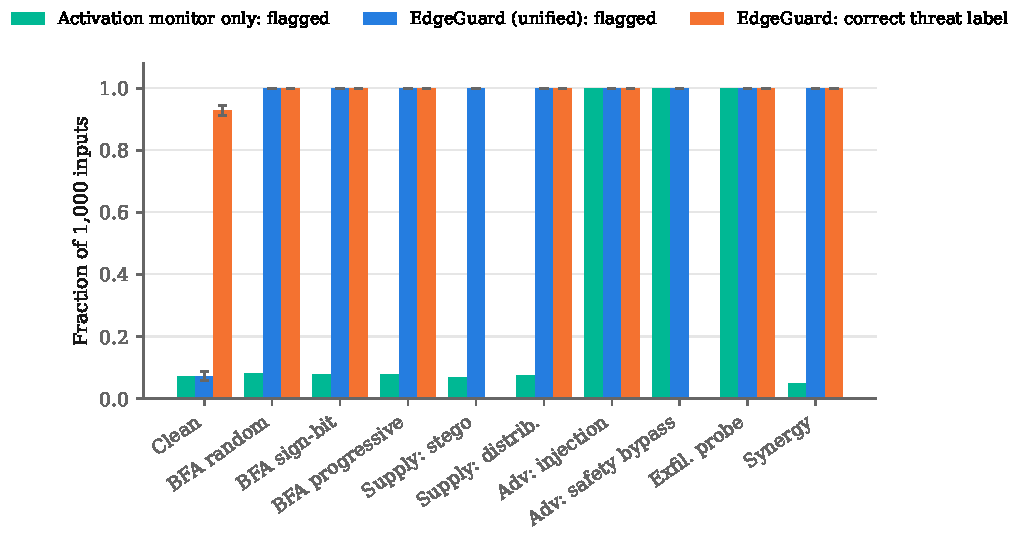
\includegraphics[width=\textwidth]{detection_by_scenario.pdf}
\caption{Per-scenario outcomes. Green: activation monitor alone. Blue: full \textsc{EdgeGuard}
pipeline. Orange: fraction receiving the intended label. Error bars: s.d.\ over seeds.}
\label{fig:detection}
\end{figure}

\Cref{tab:results} and \cref{fig:detection} summarise the outcomes. Three patterns stand out
and are examined in turn below. All weight-modifying scenarios are flagged on every input, while
the monitor alone flags them at roughly its clean false-positive rate. All activation-level
scenarios are flagged on every input by both. And label accuracy is perfect in six of the nine
attack scenarios but zero in two.

% ---------------------------------------------------------------------------
\section{RQ1: weight integrity and localisation}
\label{sec:eval:rq1}

Every input in the six weight-modifying scenarios was flagged: \FlagBfaRandom{} for random bit
flips, \FlagBfaSignBit{} for sign-bit flips, \FlagBfaProgressive{} for progressive flips,
\FlagSupplySteg{} for steganographic LSB poisoning, \FlagSupplyDistributed{} for distributed
poisoning and \FlagSynergy{} for synergy attacks. The tensors reported as tampered matched the
byte-level ground truth exactly in every case. This includes the distributed scenario, where up
to all \TinyLayers{} tensors change, and the steganographic scenario, where only up to 16
least-significant bits of one tensor change.

These results confirm \cref{prop:integrity,prop:localise} empirically, but they should not be
over-read. They are a correctness check of the implementation, not a discovery. Any change to a
byte changes a SHA-256 digest. The value of the experiment lies in confirming that the
implementation hashes what it should, in the right order, with the shape included, and that
localisation is exact for every attack pattern the simulators produce.

The monitor-only column shows the other side. Weight attacks leave the simulated activations
untouched, because the simulators do not propagate weight changes into activations, so the
monitor flags these inputs at rates between \MonSupplySteg{} and \MonBfaRandom{},
indistinguishable from its clean rate of \MonClean{}. In a real model, a damaging bit flip would usually perturb activations
downstream, but a carefully chosen one might not. Attestation does not depend on that question.

% ---------------------------------------------------------------------------
\section{RQ2: activation anomalies and the false-positive rate}
\label{sec:eval:fpr}

\subsection{Separation of attack activations}

The monitor flagged \MonAdvTextInjection{} of text-injection inputs, \MonAdvSafetyBypass{} of
safety-bypass inputs and \MonExfilProbe{} of extraction probes. The ROC curves of the
input-level maximum $|z|$ statistic (\cref{fig:roc}) have an AUC of 1.00 for all three. The
attack and clean score distributions do not overlap at all.

\begin{figure}[t]
\centering
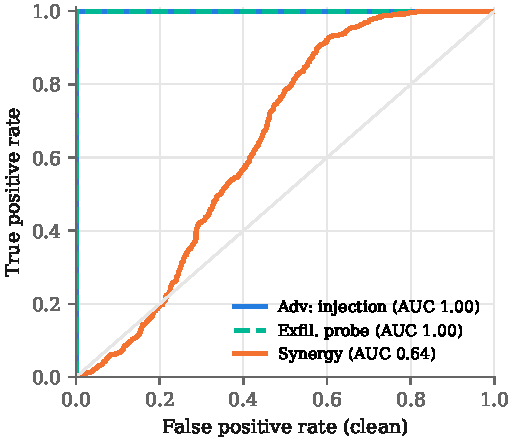
\includegraphics[width=0.62\textwidth]{roc_activation_monitor.pdf}
\caption{ROC curves of the maximum $|z|$ statistic, attack inputs against clean inputs
(\NPerScenario{} each). The safety-bypass curve coincides with the text-injection curve and is
omitted.}
\label{fig:roc}
\end{figure}

\begin{figure}[t]
\centering
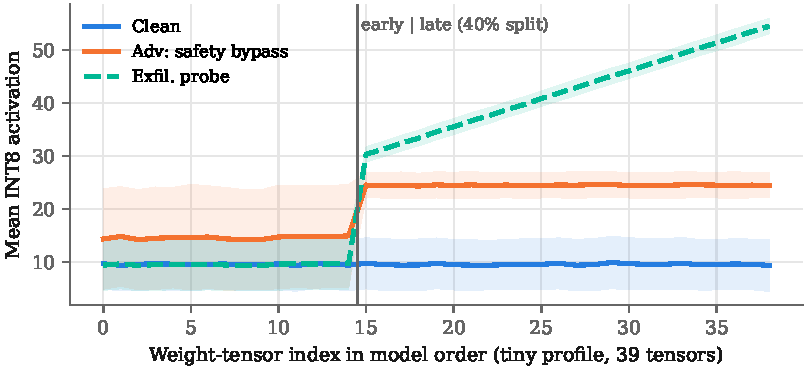
\includegraphics[width=\textwidth]{activation_profiles.pdf}
\caption{Mean INT8 activation per tensor index (50 samples; bands $\pm1$ s.d.) for clean
inputs, safety-bypass inputs and extraction probes, as produced by the simulators.}
\label{fig:profiles}
\end{figure}

Perfect separation is expected given how the attacks are simulated, and \cref{fig:profiles}
shows why. Text injection and safety bypass inflate the early-layer standard deviation from 5 to
12.5 and 10 respectively, so each early channel has a probability of several per cent of exceeding
$|z|=4$, and with 15 early layers of 32 channels at least one almost surely does. The extraction
probe moves late-layer means to between 15 and 55, which is up to nine clean standard deviations
from the clean mean of 10. A maximum-$z$ detector cannot miss either pattern. The experiment shows that the scoring and
decision path works. It does not show that real adversarial inputs or real extraction probes
produce shifts of this size. Real adversarial perturbations are typically optimised to be
small, and an adaptive attacker would aim to stay inside the calibration region
(\cref{sec:disc:adaptive}).

\subsection{The false-positive rate is a multiple-comparisons effect}

On clean inputs the pipeline raised an alarm on \FlagClean{} of inputs (\cref{tab:results}).
Of the clean inputs, \CleanAdvFrac{} were labelled ADVERSARIAL\_INPUT and \CleanTFFrac{}
TRANSIENT\_FAULT. A 7\% false-positive rate would be unacceptable in deployment, so its cause
matters.

Each monitored channel is compared against $\tau_z=4$. Under a Gaussian model, a single channel
exceeds this two-sided threshold with probability $\PSingleZFour$, but an input is flagged if any
of its $m=\MChannels$ channels does. \Cref{eq:fwer} then predicts a false-positive rate of
\PredFPRZFour{}. The measured rate was \EmpFPRZFour{}. \Cref{fig:fpr} compares the predicted and
measured rates across all thresholds from 2.5 to 6. The two curves nearly coincide, which shows
that the false-positive rate is almost entirely explained by the number of comparisons, with
channel independence and approximate Gaussianity holding well in this simulation.

\begin{figure}[t]
\centering
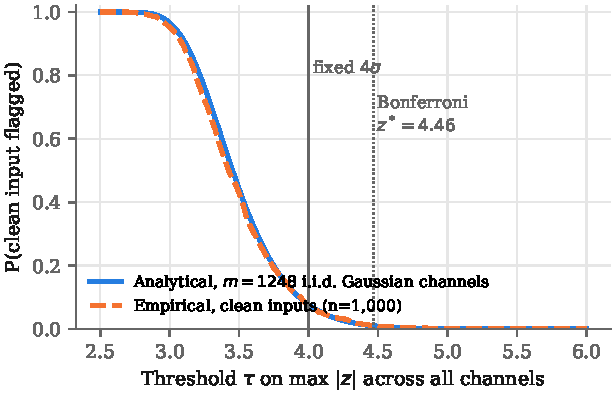
\includegraphics[width=0.75\textwidth]{fpr_multiple_comparisons.pdf}
\caption{Probability that a clean input is flagged by the $z$ test, as a function of the
threshold. Analytical: \cref{eq:fwer} with $m=\MChannels$. Empirical: \NPerScenario{} clean
inputs. Vertical lines: the default $\tau_z=4$ and the Bonferroni threshold for $\alpha=1\%$.}
\label{fig:fpr}
\end{figure}

\begin{figure}[t]
\centering
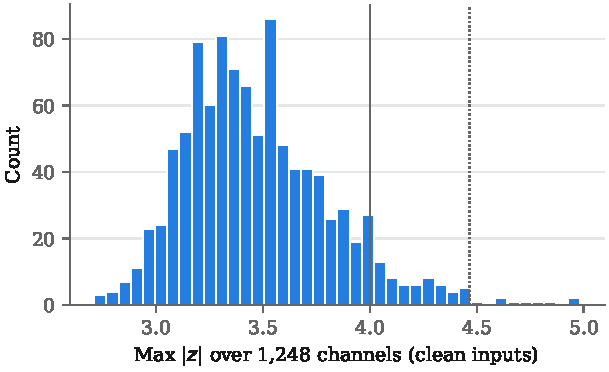
\includegraphics[width=0.7\textwidth]{clean_maxz_histogram.pdf}
\caption{Distribution of the input-level maximum $|z|$ over \MChannels{} channels for clean
inputs. Solid line: $\tau_z=4$; dotted line: $z^*=\ZBonf$.}
\label{fig:maxz}
\end{figure}

\Cref{fig:maxz} shows the same effect directly. For clean inputs the maximum $|z|$ over all
channels averaged \CleanMaxZMean{}, close to the \ExpMaxGauss{} expected for the largest of
\MChannels{} standard-normal magnitudes, and its 99th percentile was \CleanMaxZPNinetyNine{}. A
threshold of 4 therefore sits inside the bulk of the clean distribution of the statistic that
the monitor actually tests.

\subsection{A corrected threshold}

The Bonferroni threshold \cref{eq:bonf} for a target input-level false-positive rate of 1\% is
$z^*=\ZBonf$. Applying it to the recorded scores gave:

\begin{itemize}[leftmargin=*]
  \item a clean false-positive rate of \EmpFPRBonf{}, against a target of 1\%;
  \item 100\% detection of text-injection, safety-bypass and extraction-probe inputs, unchanged;
  \item \SynergyTPRBonf{} monitor-only detection of synergy inputs.
\end{itemize}

Because the activation-level attacks are so strongly separated, the threshold can be raised
without loss in this simulation. The general lesson does not depend on the simulation: a
detector that takes a maximum over many channels must set its threshold for the maximum, not for
a single channel. Doing so requires only the channel count. Monitoring a real language model,
with thousands of channels per layer and dozens of layers, would push $m$ into the hundreds of
thousands, and a per-channel $4\sigma$ rule would flag almost every input. The corrected threshold
grows only slowly with $m$, roughly as $\sqrt{2\ln m}$.

% ---------------------------------------------------------------------------
\section{RQ3: complementarity and the synergy attack}
\label{sec:eval:synergy}

The synergy scenario combines a targeted sign-bit flip with a safety-bypass input whose
activations are blended toward clean ones. The monitor alone flagged \MonSynergy{} of synergy
inputs, below its own clean false-positive rate of \MonClean{}. The blend pulls early layers back
to approximately the clean distribution, and it leaves late layers at a mean near 19 with a
standard deviation near 2. That is about two clean standard deviations above the mean but with
\emph{less} spread than clean data, so extreme channels are rarer than on clean inputs. The ROC AUC of the $|z|$ statistic against clean inputs was \AUCSynergy{}
(\cref{fig:roc}): the blended activations sit slightly above the clean distribution but overlap
it heavily. At the Bonferroni threshold, monitor-only detection fell to \SynergyTPRBonf{}. The
full pipeline flagged \FlagSynergy{} of synergy inputs and labelled all of them WEIGHT\_TAMPER,
because attestation sees the flipped bit regardless of the activations.

This is the complementarity predicted in \cref{sec:design:complement}. It is a demonstration
rather than an empirical finding about real attackers: the simulator sets the degree of
suppression directly. The result shows that the pipeline is wired so that weight evidence
overrides weak activation evidence, and that an activation monitor alone would have missed these
inputs.

% ---------------------------------------------------------------------------
\section{RQ4: threat labels}
\label{sec:eval:labels}

\begin{figure}[t]
\centering
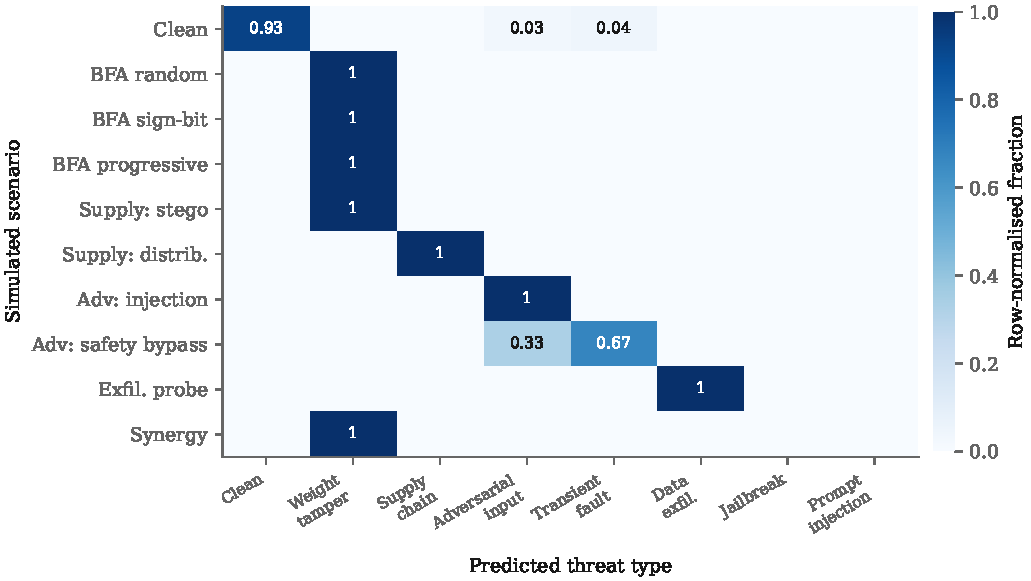
\includegraphics[width=\textwidth]{confusion_matrix.pdf}
\caption{Row-normalised confusion matrix of scenario (rows) against assigned label (columns),
\NPerScenario{} inputs per row. Raw counts are in \cref{app:results}.}
\label{fig:confusion}
\end{figure}

\Cref{fig:confusion} shows the full label distribution. Six of the nine attack scenarios received
their intended label on every input: the three bit-flip strategies (WEIGHT\_TAMPER),
distributed poisoning (SUPPLY\_CHAIN\_BACKDOOR), text injection (ADVERSARIAL\_INPUT) and
extraction probes (TRAINING\_DATA\_EXFILTRATION). Synergy inputs were labelled WEIGHT\_TAMPER,
which is the intended label because the weight evidence takes priority. Two scenarios were
labelled wrongly every time, for different reasons.

\paragraph{Steganographic poisoning was labelled WEIGHT\_TAMPER.} The supply-chain label requires
more than 30\% of tensors to be modified, and the steganographic simulator modifies one. From the
weights alone, a single modified tensor looks exactly like a runtime bit flip. This is a
limitation of the rule rather than a defect in its implementation: weights carry no record of
when or how they were changed. Distinguishing supply-chain tampering from runtime tampering
would require temporal evidence. For example, verifying at load time and again periodically
would separate weights that were wrong from the start from weights that changed in memory. With
that information, the label could be assigned correctly even for one-tensor modifications.

\paragraph{Safety-bypass inputs were never labelled JAILBREAK.} \SafetyAdvFrac{} were labelled
ADVERSARIAL\_INPUT and \SafetyTFFrac{} TRANSIENT\_FAULT. Two separate issues combine here.
\begin{enumerate}[leftmargin=*]
  \item The JAILBREAK and PROMPT\_INJECTION labels require the late-layer entropy to fall below
        0.30. The safety-bypass simulator shifts late activations upward and narrows them, but
        the entropy of \cref{eq:entropy} is invariant to shifts and to rescaling, and the
        simulated activations never come close to the threshold. The entropy branch was
        therefore never taken in any scenario. Either the score or the simulator, or both, would
        need redesign before this branch could be evaluated.
  \item Falling through to the base classifier, the early share decides the label. The 15 early
        layers, with standard deviation 10, are essentially always anomalous. The 24 late layers,
        at mean 25 and standard deviation 2.5, sit about three clean standard deviations above
        the mean, and each crosses $\tau_z=4$ only when one of its channels lands in the upper
        tail. With $k$ anomalous late layers, the early share is $15/(15+k)$, and the label is
        ADVERSARIAL\_INPUT only if $k\le15$. The split of roughly one third to two thirds
        reflects how often more than 15 late layers cross the threshold. It is the bias
        anticipated in \cref{sec:design:classifier}: the more thoroughly an input disturbs the
        network, the more likely it is to be called a fault.
\end{enumerate}
Comparing the anomaly \emph{rate} among early layers with that among late layers, rather than the
share of anomalies that are early, would label inputs that are anomalous everywhere as
adversarial rather than as faults. This change, together with a redesigned entropy score, is part
of the plan in \cref{ch:conclusion}.

\paragraph{Clean false positives were split} between ADVERSARIAL\_INPUT (\CleanAdvFrac{}) and
TRANSIENT\_FAULT (\CleanTFFrac{}), in roughly the ratio of early to late layers. This is
consistent with false alarms caused by single extreme channels located uniformly at random.

% ---------------------------------------------------------------------------
\section{RQ5: cost}
\label{sec:eval:cost}

\subsection{Per-inference latency on the tiny profile}

\begin{figure}[t]
\centering
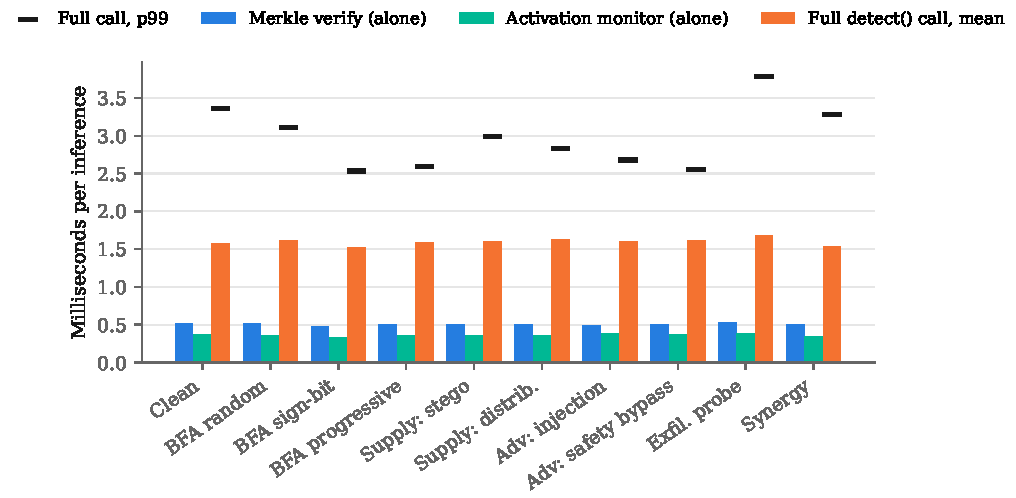
\includegraphics[width=\textwidth]{latency_breakdown.pdf}
\caption{Per-inference latency on the tiny profile: attestation alone, monitoring alone and the
full \code{detect()} call (mean, with p99 marked).}
\label{fig:latency}
\end{figure}

\Cref{fig:latency} breaks down the latency. The full \code{detect()} call took between
\LatMin{} and \LatMax{}\,ms on average across scenarios, with p99 values of at most \LatPMax{}\,ms. Attestation
alone took about \AttClean{}\,ms, which covers re-hashing all \TinyLayers{} tensors (about
0.36\,MiB) and one ECDSA verification of the reference root.
Monitoring alone took about \MonMsClean{}\,ms for \TinyLayers{} layers with $32\times32$
covariance products. The remaining time of the full call, a little under half, is spent in the
LLM scores, the classifier and building explanation strings. That share is pure overhead of the
prototype and could be reduced, for example by building explanations only when an alarm is
raised.

\subsection{Attestation cost at language-model scale}
\label{sec:eval:merkle}

\begin{table}[t]
\centering
\caption{Attestation cost on stub weight sets of increasing size (mean of three verifications;
single-threaded, 2-vCPU x86 container). The last column confirms that a single-bit change in the
last block's \code{down\_proj} was detected and localised to that tensor.}
\label{tab:merkle}
\small
\resizebox{\textwidth}{!}{% AUTO-GENERATED
\begin{tabular}{lrrrrrc}
\toprule
\textbf{Stub profile} & \textbf{Tensors} & \textbf{Params} & \textbf{MiB} & \textbf{Build (ms)} & \textbf{Verify (ms)} & \textbf{1-bit tamper localised} \\
\midrule
TinyLLM-INT8 & 39 & 366{,}144 & 0.3 & 0.7 & 0.4 & yes \\
Qwen2.5-0.5B-INT8 & 219 & 627{,}387{,}264 & 598.3 & 661.8 & 575.6 & yes \\
Llama-3.2-1B-INT8 & 147 & 1{,}469{,}122{,}560 & 1401.1 & 1605.7 & 1578.3 & yes \\
\bottomrule
\end{tabular}
}
\end{table}

\begin{figure}[t]
\centering
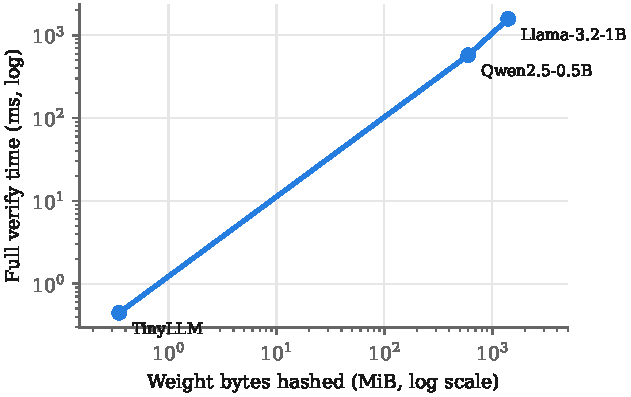
\includegraphics[width=0.65\textwidth]{merkle_scaling.pdf}
\caption{Full attestation time against the number of weight bytes hashed (log--log). Time is
linear in bytes, at roughly \MerkThrMin{}--\MerkThrMax{}\,MiB/s on this machine.}
\label{fig:merkle_scaling}
\end{figure}

\Cref{tab:merkle} and \cref{fig:merkle_scaling} report full build and verify times for three stub
profiles. Verification time is linear in the number of bytes, at \MerkThrMin{}--\MerkThrMax{}\,MiB/s
for the larger sets, which is SHA-256 throughput on one core. Verifying the Qwen2.5-0.5B stub
(\MerkSizeQwenPPB{}\,MiB) took \MerkVerQwenPPB{}\,ms; verifying the Llama-3.2-1B stub
(\MerkSizeLlamaPB{}\,MiB) took \MerkVerLlamaPB{}\,ms. A single-bit modification was detected and
localised correctly in all three.

These numbers settle RQ5 in one direction. Full re-attestation on every inference is practical
for small models but not for language models. An on-device LLM generating tokens at tens of
milliseconds per token cannot afford a 1.6-second hash pass per token. Even with hardware SHA
extensions several times faster than this container, full attestation must be amortised.
\Cref{sec:disc:amortise} discusses how the Merkle structure supports this.

% ---------------------------------------------------------------------------
\section{Fidelity of simulated weight extraction}
\label{sec:eval:extraction}

\begin{table}[t]
\centering
\caption{Cosine similarity between the dequantized extracted weights and the originals, averaged
over the tiny profile's tensors and \NSeeds{} seeds.}
\label{tab:extraction}
\small
% AUTO-GENERATED
\begin{tabular}{lrr}
\toprule
\textbf{Channel model} & \textbf{Mean cosine fidelity} & \textbf{Std.\ over seeds} \\
\midrule
Memory dump (no noise) & 1.00000 & 0.0e+00 \\
Cold boot (0.2\% single-bit decay) & 0.98772 & 7.2e-03 \\
EM side channel (2.5\% $\pm 1$ LSB) & 0.99999 & 3.0e-07 \\
\bottomrule
\end{tabular}

\end{table}

\Cref{tab:extraction} reports how closely each simulated extraction channel reproduces the
weights. A memory dump is exact. The EM channel model, which perturbs 2.5\% of weights by one
LSB, still yields a cosine similarity of \FidEmSideChannel{}, because a one-LSB error on a value
of typical magnitude around 25 is tiny. The cold-boot model, which flips one random bit in 0.2\%
of bytes, yields \FidColdBoot{}. It perturbs fewer weights, but its flips include high-order
and sign bits, each worth up to 128 units. An earlier version of this experiment, before the fix
in \cref{sec:impl:bugs}, saturated sign-bit decays instead of wrapping them, which distorts
exactly this comparison.

The practical reading is that an attacker who can read DRAM even imperfectly obtains an
essentially faithful copy of an INT8 model. Error rates would have to be far higher than those
modelled here before the copy became useless. This supports the case for confidentiality
mechanisms such as Amulet \cite{mao2025amulet}, which \textsc{EdgeGuard} does not provide.

% ---------------------------------------------------------------------------
\section{Summary}
\label{sec:eval:summary}

\begin{table}[t]
\centering
\caption{Answers to the research questions, with the strength of the evidence.}
\label{tab:rq_summary}
\small
\begin{tabularx}{\textwidth}{@{}p{1.2cm}Xp{3.2cm}@{}}
\toprule
\textbf{RQ} & \textbf{Finding} & \textbf{Evidence} \\
\midrule
RQ1 & All weight modifications detected; modified tensors localised exactly. & Strong; independent of simulation. \\
RQ2 & Simulated attacks separated perfectly. A fixed $4\sigma$ rule gives a \EmpFPRZFour{} FPR, explained by multiple comparisons; Bonferroni gives \EmpFPRBonf{}. & FPR analysis strong; separation limited by simulation. \\
RQ3 & Synergy inputs evade the monitor (\MonSynergy{}) but not the combined pipeline (\FlagSynergy{}). & Demonstration; suppression set by simulator. \\
RQ4 & Intended label in 6 of 9 attack scenarios. Steganographic poisoning indistinguishable from BFA; jailbreak branch unreachable; early/late rule biased. & Strong for the identified failures. \\
RQ5 & Detection call 1.5--1.7\,ms on tiny model. Attestation at \MerkThrMin{}--\MerkThrMax{}\,MiB/s, 1.6\,s for 1.4\,GiB: per-inference attestation infeasible for LLMs. & Strong on this machine; NPU untested. \\
\bottomrule
\end{tabularx}
\end{table}

\Cref{tab:rq_summary} collects the answers. The strongest results are those that do not depend
on how activations were simulated: exact detection and localisation of weight changes, the
explanation of the false-positive rate and its correction, and the cost of attestation at scale.
The activation-level detection rates and the synergy result show that the pipeline works as
designed, but they need real-model data before they can support claims about real attacks.

\chapter{Discussion}
\label{ch:discussion}

The evaluation separated results that hold regardless of how activations were simulated from
results that depend on it. This chapter examines what follows for deployment and for the next
phase. \Cref{sec:disc:validity} discusses threats to validity. \Cref{sec:disc:adaptive}
considers an adaptive attacker. \Cref{sec:disc:toctou,sec:disc:amortise} address the timing and
cost of attestation. \Cref{sec:disc:llm} discusses what changes for real language models, and
\cref{sec:disc:labels} the role of labels. \Cref{sec:disc:ethics} closes with ethical
considerations.

% ---------------------------------------------------------------------------
\section{Threats to validity}
\label{sec:disc:validity}

\paragraph{Construct validity: simulated activations.} The largest threat is that activation-level
attacks are defined as Gaussian distributions that differ from the clean Gaussian in mean or
spread. The monitor models the clean Gaussian. Detection of such attacks is close to guaranteed
whenever the difference is large, and impossible when it is small, so the measured rates reflect
choices made in the simulator. Real activations are not Gaussian. Transformer activations in
particular are known to contain large outliers in a few channels, the problem SmoothQuant
addresses \cite{xiao2023smoothquant}. Such outliers would inflate the clean $z$ distribution and
force higher thresholds, and per-channel normalisation would be essential.

\paragraph{Internal validity: shared authorship.} The detector, the simulators and the evaluation
were written together. The two defects of \cref{sec:impl:bugs} that sat in the simulators, and
the covariance defect that sat in the detector, show that such a pipeline can hide errors.
Independent references in the tests mitigate this risk, and the fact that the clean false-positive
rate matches a closed-form prediction is reassuring, because a gross error in the scoring path
would break that agreement.

\paragraph{External validity: stub weights and the test machine.} The weight sets have
realistic tensor shapes but random contents. Attestation cost depends only on byte count, so the
scaling results transfer to real checkpoints of the same size. They do not transfer to the NPU
or to a phone CPU, whose SHA-256 throughput may be higher, with hardware extensions, or lower.

\paragraph{Statistical conclusion validity.} With \NPerScenario{} inputs per scenario, a measured
rate of 100\% has a one-sided 95\% lower confidence bound of about 99.7\%, by the ``rule of
three''. A measured rate of 0\% has an upper bound of about 0.3\%. These bounds are adequate for
the claims made. The false-positive comparison (predicted \PredFPRZFour{}, measured \EmpFPRZFour{}
with a seed-to-seed standard deviation of 1.5 points) is consistent within sampling error.

% ---------------------------------------------------------------------------
\section{An adaptive attacker}
\label{sec:disc:adaptive}

Suppose the attacker knows the calibration statistics and thresholds. The two detectors respond
very differently.

\paragraph{Against attestation,} knowledge does not help. Evading it requires a SHA-256 second
preimage for a modified tensor, a forged ECDSA signature, or control of the verifier, and all
three are excluded by the threat model. The realistic adaptive strategies are temporal rather than
cryptographic: flip bits just after a verification and restore them before the next one, or
attack between verifications (\cref{sec:disc:toctou}).

\paragraph{Against the monitor,} knowledge helps a great deal. An attacker optimising an
adversarial input can add a penalty that keeps every monitored channel's $|z|$ below $\tau_z$ and
every Mahalanobis distance below $\tau_D$. Whether a successful attack remains feasible under that
constraint depends on how much freedom the input space leaves once activations are confined to the
calibration region. Carlini and Wagner showed that ten published adversarial-example detectors could
each be bypassed by attacks constructed with knowledge of the detector
\cite{carlini2017bypassing}. The honest default assumption is that a single-statistic monitor will not stop a determined adaptive
attacker. Its realistic roles are to raise the cost of attacks, to catch non-adaptive ones such as
off-the-shelf jailbreak prompts and faults, and to provide forensic signal.

Three directions could make the monitor harder to evade, and each is a candidate for the next
phase. First, keeping the set of monitored layers or channels secret and rotating it would force
the attacker to satisfy constraints on everything. Second, statistics that are expensive to
satisfy jointly, such as the joint distribution across layers, could replace per-layer marginals.
Third, the monitor could be coupled to the model's output, so that inputs that change the output a
great deal while keeping activations typical become suspicious.

% ---------------------------------------------------------------------------
\section{Time of check versus time of use}
\label{sec:disc:toctou}

Attestation certifies the weights at the moment they are hashed. If verification runs at times
$t_1<t_2<\dots$ and inference reads weights at $t$, a flip at $t_1<t'<t$ affects that inference
undetected, and it is caught only at the next verification. Two quantities therefore matter: the
\emph{detection latency}, the time from a flip to the next verification that covers the modified
tensor, and the \emph{exposure}, the number of inferences that run on modified weights in the
meantime.

Closing the gap completely would require verifying the bytes on the path into the accelerator,
for example by hashing in the DMA engine or in on-chip SRAM after transfer. That is a hardware
change. For a software-only design, the realistic goal is a bounded
detection latency at an acceptable cost, the subject of the next section.

% ---------------------------------------------------------------------------
\section{Amortised attestation}
\label{sec:disc:amortise}

\Cref{sec:eval:merkle} measured \MerkVerLlamaPB{}\,ms to verify the 1.4\,GiB Llama-3.2-1B stub.
Suppose a budget of $b$ seconds of hashing per inference step, and hashing throughput $\rho$
bytes per second. Each step can verify $b\rho$ bytes. The Merkle tree makes partial verification
sound: any subset of tensors can be checked against the signed root using their membership
proofs (\cref{fig:merkle}), without hashing the rest.

\paragraph{Round-robin verification.} Verify tensors in a fixed cyclic order, $b\rho$ bytes per
step. A full cycle covering all $B$ bytes takes $\lceil B/(b\rho)\rceil$ steps, and every
modification is detected within one cycle. At the measured $\rho\approx\MerkThrLlamaPB$\,MiB/s and a budget of
$b=5$\,ms per token, $b\rho\approx 4.5$\,MiB per token, and the Llama-3.2-1B stub
($B\approx\MerkSizeLlamaPB$\,MiB) is fully covered every $\approx315$ tokens. An attacker who
knows the schedule can, however, time a flip-and-restore to avoid it.

\paragraph{Randomised verification.} Choose each step's tensors at random, weighted by size, with
the choice secret. A modified tensor of $\beta$ bytes is covered in a given step with probability
about $q = \min(1, b\rho/B)$ if verification is byte-proportional, and it remains undetected
after $t$ steps with probability $(1-q)^t$. With the numbers above, $q\approx 1/315$. A
modification persisting for 1{,}000 tokens escapes detection with probability
$(1-1/315)^{1000}\approx 4\%$, and one persisting for 2{,}000 tokens with probability about
0.2\%. Randomisation removes the attacker's ability to predict the schedule at the cost of a
probabilistic rather than deterministic bound. Combining the two, a random permutation per cycle,
gives a deterministic bound of one cycle with unpredictable timing within it.

\paragraph{Prioritised verification.} Not all tensors matter equally. Hong et al.\ found that a
large fraction of single-bit vulnerabilities concentrate in particular parameters
\cite{hong2019terminal}, HASHTAG selects layers by measured sensitivity
\cite{javaheripi2021hashtag}, and NeuroPots steers attacks into known trapdoors
\cite{liu2023neuropots}. Verifying sensitive tensors more often shortens their detection latency
at no extra cost. For transformers, the embedding and output projections are a large share of
the bytes ($2VH$ in \cref{eq:stub_params}, about 36\% of the Llama-3.2-1B stub's parameters). Their
sensitivity to single flips relative to the attention and MLP projections is an open empirical
question that the next phase can measure on a real model.

\paragraph{Faster hashing.} SHA-256 throughput on CPUs with SHA extensions is typically several
times higher than the \MerkThrMin{}--\MerkThrMax{}\,MiB/s measured on this container. A non-cryptographic
checksum as a first-line filter, with cryptographic verification only on a schedule, is the
trade-off RADAR and HASHTAG make \cite{li2021radar,javaheripi2021hashtag}. Such a filter must be
keyed, or its positions secret, because an attacker who knows an unkeyed checksum can flip
compensating bits. A keyed MAC computed with a key held in the TEE retains cryptographic strength
and is typically faster than a hash plus a signature check.

% ---------------------------------------------------------------------------
\section{From stubs to real language models}
\label{sec:disc:llm}

Moving the monitor to a real quantized LLM changes four things.

\begin{enumerate}[leftmargin=*]
  \item \textbf{Channel count.} A model with hidden size 2048 and 16 blocks, monitored at two
        points per block, has $m\approx 65{,}000$ channels per token. \Cref{eq:bonf} gives
        $z^*\approx 5.25$ for $\alpha=1\%$, compared with \ZBonf{} here. The correction remains
        cheap to compute, but every attack signal must exceed a higher bar.
  \item \textbf{Covariance.} A dense $2048\times2048$ covariance per monitoring point is 32\,MiB
        in double precision. Diagonal statistics, low-rank-plus-diagonal models, or projection
        onto a few principal components are the realistic options.
  \item \textbf{Tokens.} A language model produces one activation vector per token. Monitoring
        can score each token, which is expensive and multiplies the comparisons, or summarise a
        sequence. Prompt-level attacks are naturally scored per sequence, generation-time
        extraction per token.
  \item \textbf{Validating the memorisation hypothesis.} The extraction-probe detector assumes
        that regurgitating memorised text produces confident, low-variance late activations. A
        direct test is possible with public tools. Take a small open model, a set of known
        memorised sequences such as those identified by extraction studies, and matched
        non-memorised controls, and compare late-layer activation statistics while the model
        generates them. If no difference appears, the memorisation score should be dropped. If
        one does, its thresholds can be fitted to data rather than to the simulator.
\end{enumerate}

% ---------------------------------------------------------------------------
\section{On threat labels}
\label{sec:disc:labels}

The classifier's labels were useful in the evaluation mainly because they failed in informative
ways. Steganographic poisoning and runtime bit flips cannot be told apart from the weights alone.
Inputs that disturb every layer were called faults. And an entropy score invariant to shifts and
scaling could not respond to the simulated jailbreak. Each failure pointed to missing evidence
rather than to a tuning problem. Provenance requires evidence over time, the fault-versus-attack
distinction requires a comparison that is not biased by layer counts, and jailbreak detection
requires a score sensitive to the property of interest.

A more robust design would make the label a function of explicitly listed evidence, such as
``hash mismatch at load time'', ``hash mismatch first seen at runtime'', ``anomaly rate in early
layers $>$ late layers'' and ``memorisation score above threshold''. The output would report the
evidence alongside a suggested interpretation, rather than collapsing everything into one of eight
names. The explanation strings already list most of this evidence. Promoting it to structured
output would let operators write their own response policies.

% ---------------------------------------------------------------------------
\section{Ethical considerations}
\label{sec:disc:ethics}

The attack simulators in this project do not implement working attacks. The bit-flip simulators
modify arrays in memory and contain no Rowhammer code. The extraction and probe simulators
generate synthetic activation distributions and recover no data. Nothing in the repository
lowers the barrier to attacking a real system beyond what the cited literature already
describes. The defensive components are intended to be published openly so that others can
evaluate and improve them.

Two downstream concerns deserve mention. A monitor that inspects activations sees, indirectly,
information about user inputs, so a deployment should not log activations or explanations
containing them without the same care applied to the inputs themselves. And false positives have
costs: a 7\% false-alarm rate that rejects legitimate requests would harm users. This is one
reason the threshold analysis of \cref{sec:eval:fpr} matters beyond the evaluation.

\chapter{Conclusion and Future Work}
\label{ch:conclusion}

\section{Summary}

This report presented \textsc{EdgeGuard}, a framework that combines signed Merkle-tree
attestation of quantized weights with an INT8 activation monitor and a rule-based threat
classifier, together with a testbed of attack simulators and language-model-shaped weight sets.
The evaluation, generated end to end from recorded runs, supports five conclusions.

\begin{enumerate}[leftmargin=*]
  \item \textbf{Cryptographic attestation does what it should, and localises exactly.} Every
        simulated weight modification was detected and attributed to exactly the tensors that
        changed, from single least-significant bits to perturbations spread over every tensor.
        This result does not depend on the simulation.
  \item \textbf{The monitor's false-positive rate is governed by the number of channels.} A
        per-channel $4\sigma$ rule over \MChannels{} channels flagged \EmpFPRZFour{} of clean
        inputs, matching the \PredFPRZFour{} predicted by \cref{eq:fwer}. A Bonferroni threshold
        reduced this to \EmpFPRBonf{} with no loss of detection in the simulated scenarios. For a
        real language model, with tens of thousands of channels, this correction is essential.
  \item \textbf{The two detectors are complementary.} Synergy inputs that kept activations near
        the clean distribution were flagged by the monitor at \MonSynergy{} and by the combined
        pipeline at \FlagSynergy{}.
  \item \textbf{The labels need better evidence, not better tuning.} Single-tensor supply-chain
        modifications cannot be distinguished from runtime flips without temporal evidence. The
        early/late rule labels pervasive input attacks as faults, and the entropy score cannot
        respond to shifted or narrowed activations.
  \item \textbf{Full attestation does not scale to per-inference use for LLMs.} At about
        \MerkThrMin{}--\MerkThrMax{}\,MiB/s, verifying 1.4\,GiB took 1.6\,s. The Merkle structure supports
        amortised verification with a deterministic bound of about 315 tokens at a 5\,ms-per-token
        budget, or probabilistic bounds under randomisation.
\end{enumerate}

Building the evaluation also uncovered three defects, two integer-width errors in the bit-flip
and cold-boot simulators and one algebraic error in the streaming covariance. Each had passed
tests that checked intended behaviour. All three were fixed and covered by regression tests
against independent references.

\section{Limitations}

The principal limitation is that activation-level results come from simulated activations whose
distributions were chosen together with the detector. They show that the pipeline functions as
designed, not that it detects real attacks. No real model was executed, no NPU was used, and no
adaptive attacker was evaluated. The memorisation score's premise, that extraction probes produce
distinctive late-layer activations, is a hypothesis that this project has not tested.

\section{Plan for the next phase}

\begin{figure}[t]
\centering
\begin{tikzpicture}[x=0.9cm, y=0.62cm]
\foreach \m/\lab in {0/Dec,1/Jan,2/Feb,3/Mar,4/Apr,5/May} {
  \node[font=\scriptsize, text=eggray] at (\m*2+1,0.7) {\lab};
  \draw[eggray!40] (\m*2,0.3) -- (\m*2,-8.4);
}
\draw[eggray!40] (12,0.3) -- (12,-8.4);
\foreach \y/\t/\s/\e/\c in {
  0/W1: label and explanation fixes/0/1/egaqua,
  1/W2: real-model activation capture (PyTorch)/0.5/3/egblue,
  2/W3: memorisation hypothesis test/2/4.5/egblue,
  3/W4: threshold calibration on real data/3/5/egblue,
  4/W5: amortised attestation + keyed MAC/3.5/6.5/egorange,
  5/W6: QNN adapter on Snapdragon device/5/9/egorange,
  6/W7: adaptive-attacker study/7/10/egblue,
  7/W8: thesis writing and submission/9.5/12/egaqua} {
  \node[font=\scriptsize, anchor=east] at (-0.1,-\y-0.6) {\t};
  \fill[\c, rounded corners=1pt] (\s,-\y-0.35) rectangle (\e,-\y-0.85);
}
\end{tikzpicture}
\caption{Indicative schedule for the next phase (December 2026 -- May 2027). Blue: evaluation on
real models; orange: systems work; aqua: fixes and writing.}
\label{fig:gantt}
\end{figure}

The next phase replaces simulation with measurement wherever possible. \Cref{fig:gantt} shows an
indicative schedule.

\begin{description}[leftmargin=*,style=nextline]
  \item[W1 — Fixes from this evaluation.] Replace the early-share rule with a comparison of
        anomaly rates; reword the signature line of explanations; bind dtype and leaf count into
        the hashes and add domain separation (\cref{rem:padding}); make Bonferroni the default
        threshold; emit structured evidence alongside labels.
  \item[W2 — Real activations.] Run a small open-weight model, quantized to INT8, under PyTorch
        with forward hooks. Capture activations from benign prompts for calibration and from
        published jailbreak and prompt-injection sets for evaluation. Measure the clean
        false-positive rate at the Bonferroni threshold on real, non-Gaussian activations.
  \item[W3 — Memorisation hypothesis.] Compare late-layer statistics during generation of known
        memorised sequences and matched controls (\cref{sec:disc:llm}). Keep, refit or drop the
        memorisation score according to the result.
  \item[W4 — Calibration on real data.] Fit thresholds with held-out empirical quantiles as well as
        Bonferroni, and compare diagonal, low-rank and full covariance models.
  \item[W5 — Amortised attestation.] Implement randomised, size-weighted partial verification with
        Merkle proofs and a keyed-MAC fast path. Measure detection latency against injected flips
        during generation.
  \item[W6 — Device integration.] Implement the QNN adapter against the Qualcomm AI Engine Direct
        SDK, expose selected intermediate tensors from the HTP backend, and measure overhead on a
        Snapdragon development device.
  \item[W7 — Adaptive attacker.] Optimise adversarial prompts against a model with the monitor's
        thresholds as a constraint, and report how much the monitor raises the attack cost.
  \item[W8 — Writing.] Consolidate the results into the final thesis and, if they warrant it, a
        workshop paper.
\end{description}

\section{Closing remark}

The most useful outcome of this phase is a clear map of where the project stands. The
cryptographic half of \textsc{EdgeGuard} is sound, and its main open problem is cost. The
statistical half is wired correctly and its false-positive behaviour is understood, but its
detection ability remains unproven until it meets real activations. The next phase is designed to
supply that evidence.


\cleardoublepage
\phantomsection
\addcontentsline{toc}{chapter}{References}
% All entries checked against publisher pages, arXiv, DBLP, Crossref, PMLR or ACL Anthology
% (November 2026). Entries marked [std] are standards documents; [doc] vendor documentation.
\begin{thebibliography}{99}
\small

\bibitem{carlini2017bypassing}
N.~Carlini and D.~Wagner, ``Adversarial examples are not easily detected: Bypassing ten detection
methods,'' in \textit{Proc.\ 10th ACM Workshop on Artificial Intelligence and Security (AISec)},
2017, pp.~3--14.

\bibitem{carlini2021extracting}
N.~Carlini, F.~Tram\`er, E.~Wallace, M.~Jagielski, A.~Herbert-Voss, K.~Lee, A.~Roberts, T.~Brown,
D.~Song, \'U.~Erlingsson, A.~Oprea, and C.~Raffel, ``Extracting training data from large language
models,'' in \textit{Proc.\ 30th USENIX Security Symposium}, 2021, pp.~2633--2650.

\bibitem{dai2025activation}
C.~Dai, L.~Lu, and P.~Zhou, ``Stealing training data from large language models in decentralized
training through activation inversion attack,'' in \textit{Proc.\ 63rd Annual Meeting of the
Association for Computational Linguistics (ACL)}, Vienna, 2025, pp.~14539--14551.
doi:10.18653/v1/2025.acl-long.707.

\bibitem{dunn1961multiple}
O.~J.~Dunn, ``Multiple comparisons among means,'' \textit{Journal of the American Statistical
Association}, vol.~56, no.~293, pp.~52--64, 1961.

\bibitem{executorch_qnn}
PyTorch ExecuTorch, ``Qualcomm AI Engine backend,'' documentation, 2026.
\url{https://docs.pytorch.org/executorch/stable/backends-qualcomm.html} [doc]

\bibitem{feng2024privacy}
S.~Feng and F.~Tram\`er, ``Privacy backdoors: Stealing data with corrupted pretrained models,'' in
\textit{Proc.\ 41st International Conference on Machine Learning (ICML)}, PMLR vol.~235, 2024,
pp.~13326--13364.

\bibitem{fips180-4}
National Institute of Standards and Technology, ``Secure Hash Standard (SHS),'' FIPS PUB 180-4,
2015. [std]

\bibitem{fips186-5}
National Institute of Standards and Technology, ``Digital Signature Standard (DSS),'' FIPS PUB
186-5, 2023. [std]

\bibitem{frantar2023gptq}
E.~Frantar, S.~Ashkboos, T.~Hoefler, and D.~Alistarh, ``GPTQ: Accurate post-training quantization
for generative pre-trained transformers,'' in \textit{Proc.\ International Conference on Learning
Representations (ICLR)}, 2023. arXiv:2210.17323.

\bibitem{goodfellow2015explaining}
I.~J.~Goodfellow, J.~Shlens, and C.~Szegedy, ``Explaining and harnessing adversarial examples,''
in \textit{Proc.\ International Conference on Learning Representations (ICLR)}, 2015.

\bibitem{guo2021modelshield}
Y.~Guo, L.~Liu, Y.~Cheng, Y.~Zhang, and J.~Yang, ``ModelShield: A generic and portable framework
extension for defending bit-flip based adversarial weight attacks,'' in \textit{Proc.\ IEEE
International Conference on Computer Design (ICCD)}, 2021.

\bibitem{halderman2008lest}
J.~A.~Halderman, S.~D.~Schoen, N.~Heninger, W.~Clarkson, W.~Paul, J.~A.~Calandrino, A.~J.~Feldman,
J.~Appelbaum, and E.~W.~Felten, ``Lest we remember: Cold boot attacks on encryption keys,'' in
\textit{Proc.\ 17th USENIX Security Symposium}, 2008, pp.~45--60.

\bibitem{he2020defending}
Z.~He, A.~S.~Rakin, J.~Li, C.~Chakrabarti, and D.~Fan, ``Defending and harnessing the bit-flip
based adversarial weight attack,'' in \textit{Proc.\ IEEE/CVF Conference on Computer Vision and
Pattern Recognition (CVPR)}, 2020.

\bibitem{hong2019terminal}
S.~Hong, P.~Frigo, Y.~Kaya, C.~Giuffrida, and T.~Dumitra\c{s}, ``Terminal brain damage: Exposing
the graceless degradation in deep neural networks under hardware fault attacks,'' in
\textit{Proc.\ 28th USENIX Security Symposium}, 2019, pp.~497--514.

\bibitem{jacob2018quantization}
B.~Jacob, S.~Kligys, B.~Chen, M.~Zhu, M.~Tang, A.~Howard, H.~Adam, and D.~Kalenichenko,
``Quantization and training of neural networks for efficient integer-arithmetic-only inference,''
in \textit{Proc.\ IEEE/CVF CVPR}, 2018, pp.~2704--2713.

\bibitem{javaheripi2021hashtag}
M.~Javaheripi and F.~Koushanfar, ``HASHTAG: Hash signatures for online detection of
fault-injection attacks on deep neural networks,'' in \textit{Proc.\ IEEE/ACM International
Conference on Computer-Aided Design (ICCAD)}, 2021, pp.~1--9. doi:10.1109/ICCAD51958.2021.9643556.

\bibitem{kim2014flipping}
Y.~Kim, R.~Daly, J.~Kim, C.~Fallin, J.~H.~Lee, D.~Lee, C.~Wilkerson, K.~Lai, and O.~Mutlu,
``Flipping bits in memory without accessing them: An experimental study of DRAM disturbance
errors,'' in \textit{Proc.\ 41st International Symposium on Computer Architecture (ISCA)}, 2014,
pp.~361--372.

\bibitem{lee2018simple}
K.~Lee, K.~Lee, H.~Lee, and J.~Shin, ``A simple unified framework for detecting out-of-distribution
samples and adversarial attacks,'' in \textit{Advances in Neural Information Processing Systems
(NeurIPS)}, 2018.

\bibitem{li2020defending}
J.~Li, A.~S.~Rakin, Y.~Xiong, L.~Chang, Z.~He, D.~Fan, and C.~Chakrabarti, ``Defending bit-flip
attack through DNN weight reconstruction,'' in \textit{Proc.\ 57th ACM/IEEE Design Automation
Conference (DAC)}, 2020.

\bibitem{li2021radar}
J.~Li, A.~S.~Rakin, Z.~He, D.~Fan, and C.~Chakrabarti, ``RADAR: Run-time adversarial weight attack
detection and accuracy recovery,'' in \textit{Proc.\ Design, Automation \& Test in Europe (DATE)},
2021, pp.~790--795. doi:10.23919/DATE51398.2021.9474113.

\bibitem{liu2023neuropots}
Q.~Liu, J.~Yin, W.~Wen, C.~Yang, and S.~Sha, ``NeuroPots: Realtime proactive defense against
bit-flip attacks in neural networks,'' in \textit{Proc.\ 32nd USENIX Security Symposium}, 2023.

\bibitem{llama3herd}
A.~Dubey \textit{et al.} (Llama Team, AI @ Meta), ``The Llama 3 herd of models,''
arXiv:2407.21783, 2024.

\bibitem{madry2018towards}
A.~Madry, A.~Makelov, L.~Schmidt, D.~Tsipras, and A.~Vladu, ``Towards deep learning models resistant
to adversarial attacks,'' in \textit{Proc.\ ICLR}, 2018.

\bibitem{mahalanobis1936}
P.~C.~Mahalanobis, ``On the generalised distance in statistics,'' \textit{Proceedings of the
National Institute of Sciences of India}, vol.~2, no.~1, pp.~49--55, 1936.

\bibitem{mao2025amulet}
Z.~Mao, L.~Zhao, L.~Xu, W.~Dong, S.~Zhang, C.~Wang, and Q.~Wang, ``Amulet: Fast TEE-shielded
inference for on-device model protection,'' arXiv:2512.07495, 2025.

\bibitem{merkle1987digital}
R.~C.~Merkle, ``A digital signature based on a conventional encryption function,'' in
\textit{Advances in Cryptology --- CRYPTO '87}, LNCS vol.~293, Springer, 1988, pp.~369--378.

\bibitem{nagel2021whitepaper}
M.~Nagel, M.~Fournarakis, R.~A.~Amjad, Y.~Bondarenko, M.~van~Baalen, and T.~Blankevoort, ``A white
paper on neural network quantization,'' arXiv:2106.08295, 2021.

\bibitem{nasr2023scalable}
M.~Nasr, N.~Carlini, J.~Hayase, M.~Jagielski, A.~F.~Cooper, D.~Ippolito, C.~A.~Choquette-Choo,
E.~Wallace, F.~Tram\`er, and K.~Lee, ``Scalable extraction of training data from (production)
language models,'' arXiv:2311.17035, 2023.

\bibitem{phi3report}
M.~Abdin \textit{et al.}, ``Phi-3 technical report: A highly capable language model locally on your
phone,'' arXiv:2404.14219, 2024.

\bibitem{qualcomm_qnn}
Qualcomm Technologies, Inc., ``Qualcomm AI Engine Direct SDK,'' product page, 2026.
\url{https://www.qualcomm.com/developer/software/qualcomm-ai-engine-direct-sdk} [doc]

\bibitem{qualcomm_qnn_backend}
Qualcomm Technologies, Inc., ``Qualcomm AI Engine Direct: Backend,'' SDK documentation
80-63442-10, 2026. \url{https://docs.qualcomm.com/bundle/publicresource/80-63442-10/topics/backend.md} [doc]

\bibitem{qwen25report}
Qwen Team (A.~Yang \textit{et al.}), ``Qwen2.5 technical report,'' arXiv:2412.15115, 2024.

\bibitem{rakin2019bfa}
A.~S.~Rakin, Z.~He, and D.~Fan, ``Bit-flip attack: Crushing neural network with progressive bit
search,'' in \textit{Proc.\ IEEE/CVF International Conference on Computer Vision (ICCV)}, 2019,
pp.~1211--1220.

\bibitem{tramer2016stealing}
F.~Tram\`er, F.~Zhang, A.~Juels, M.~K.~Reiter, and T.~Ristenpart, ``Stealing machine learning
models via prediction APIs,'' in \textit{Proc.\ 25th USENIX Security Symposium}, 2016,
pp.~601--618.

\bibitem{vaswani2017attention}
A.~Vaswani, N.~Shazeer, N.~Parmar, J.~Uszkoreit, L.~Jones, A.~N.~Gomez, \L.~Kaiser, and
I.~Polosukhin, ``Attention is all you need,'' in \textit{Advances in Neural Information Processing
Systems (NeurIPS)}, 2017.

\bibitem{welford1962note}
B.~P.~Welford, ``Note on a method for calculating corrected sums of squares and products,''
\textit{Technometrics}, vol.~4, no.~3, pp.~419--420, 1962.

\bibitem{wen2024privacy}
Y.~Wen, L.~Marchyok, S.~Hong, J.~Geiping, T.~Goldstein, and N.~Carlini, ``Privacy backdoors:
Enhancing membership inference through poisoning pre-trained models,'' arXiv:2404.01231, 2024.

\bibitem{xiao2023smoothquant}
G.~Xiao, J.~Lin, M.~Seznec, H.~Wu, J.~Demouth, and S.~Han, ``SmoothQuant: Accurate and efficient
post-training quantization for large language models,'' in \textit{Proc.\ 40th ICML}, PMLR
vol.~202, 2023.

\bibitem{yao2020deephammer}
F.~Yao, A.~S.~Rakin, and D.~Fan, ``DeepHammer: Depleting the intelligence of deep neural networks
through targeted chain of bit flips,'' in \textit{Proc.\ 29th USENIX Security Symposium}, 2020,
pp.~1463--1480.

\end{thebibliography}


\appendix
\chapter{Configuration File}
\label{app:config}

The default configuration shipped with the package (\code{configs/default.yaml}) is reproduced
below. The evaluation in \cref{ch:evaluation} constructs its components programmatically with the
parameters stated in \cref{sec:eval:setup}. In particular, it uses $\tau_D=50$ rather than the
file's default of 25.

\lstinputlisting[language={},numbers=left,frame=single,basicstyle=\ttfamily\scriptsize]{../../configs/default.yaml}

% ---------------------------------------------------------------------------
\chapter{API Reference}
\label{app:api}

This appendix lists the public classes, methods and functions of each module, with signatures
and the first line of each docstring. It is generated by \code{experiments/make\_api\_doc.py}
through introspection of the source, so it matches the code at the time the report was built.

{\small\sloppy\raggedright
% AUTO-GENERATED by experiments/make_api_doc.py
\subsection*{\texttt{edgeguard.attestation.merkle}}
\begin{itemize}[leftmargin=*,itemsep=1pt]
\item \textbf{class \texttt{MerkleNode}} --- A single node in the Merkle tree.
\item \textbf{class \texttt{MerkleTree}} --- Binary Merkle tree built over a sequence of layer weight hashes.
\begin{itemize}[leftmargin=1.2em,itemsep=0pt]
\item \texttt{\small from\_\allowbreak{}dict(\allowbreak{}data: 'dict') -> "'MerkleTree'"} --- Reconstruct a MerkleTree from to\_dict() output.
\item \texttt{\small from\_\allowbreak{}hashes(\allowbreak{}layer\_\allowbreak{}hashes: 'Sequence[bytes]') -> "'MerkleTree'"} --- Build from pre-computed 32-byte leaf hashes (e.g. loaded from disk).
\item \texttt{\small from\_\allowbreak{}weights(\allowbreak{}layer\_\allowbreak{}weights: 'dict[str,\allowbreak{} np.ndarray]') -> "'MerkleTree'"} --- Hash each weight tensor and build the Merkle tree.
\item \texttt{\small get\_\allowbreak{}proof(\allowbreak{}self,\allowbreak{} leaf\_\allowbreak{}index: 'int') -> 'list[tuple[str,\allowbreak{} bytes]]'} --- Return the Merkle inclusion proof for a given leaf.
\item \texttt{\small to\_\allowbreak{}dict(\allowbreak{}self) -> 'dict'} --- Serialize the tree's leaf hashes to a JSON-compatible dict.
\item \texttt{\small verify\_\allowbreak{}and\_\allowbreak{}localize(\allowbreak{}self,\allowbreak{} fresh\_\allowbreak{}hashes: 'Sequence[bytes]') -> 'tuple[bool,\allowbreak{} list[int]]'} --- Compare fresh layer hashes against the stored tree.
\end{itemize}
\end{itemize}
\subsection*{\texttt{edgeguard.attestation.manager}}
\begin{itemize}[leftmargin=*,itemsep=1pt]
\item \textbf{class \texttt{AttestationResult}} --- Return value from MerkleAttestationManager.verify().
\begin{itemize}[leftmargin=1.2em,itemsep=0pt]
\item \texttt{\small summary(\allowbreak{}self) -> 'str'}
\end{itemize}
\item \textbf{class \texttt{MerkleAttestationManager}} --- Manages the full lifecycle of Merkle-tree-based weight attestation.
\begin{itemize}[leftmargin=1.2em,itemsep=0pt]
\item \texttt{\small build(\allowbreak{}self,\allowbreak{} layer\_\allowbreak{}weights: 'dict[str,\allowbreak{} np.ndarray]',\allowbreak{} private\_\allowbreak{}key=None) -> 'bytes'} --- Hash all layer weight tensors, build the Merkle tree, sign the root.
\item \texttt{\small load(\allowbreak{}path: 'str | Path') -> "'MerkleAttestationManager'"} --- Load an attestation previously saved with save().
\item \texttt{\small save(\allowbreak{}self,\allowbreak{} path: 'str | Path') -> 'None'} --- Persist the attestation state to a JSON file.
\item \texttt{\small verify(\allowbreak{}self,\allowbreak{} layer\_\allowbreak{}weights: 'dict[str,\allowbreak{} np.ndarray]') -> 'AttestationResult'} --- Verify the integrity of the model weights.
\end{itemize}
\end{itemize}
\subsection*{\texttt{edgeguard.detection.statistics}}
\begin{itemize}[leftmargin=*,itemsep=1pt]
\item \textbf{class \texttt{LayerStats}} --- Calibration statistics for one layer, computed over INT8 activations.
\begin{itemize}[leftmargin=1.2em,itemsep=0pt]
\item \texttt{\small from\_\allowbreak{}dict(\allowbreak{}data: 'dict') -> "'LayerStats'"}
\item \texttt{\small to\_\allowbreak{}dict(\allowbreak{}self) -> 'dict'}
\end{itemize}
\item \textbf{class \texttt{StreamingInt8Stats}} --- Online (streaming) computation of mean, variance, and covariance
\begin{itemize}[leftmargin=1.2em,itemsep=0pt]
\item \texttt{\small finalize(\allowbreak{}self) -> 'LayerStats'} --- Compute final statistics and return a LayerStats object.
\item \texttt{\small update(\allowbreak{}self,\allowbreak{} activation: 'np.ndarray') -> 'None'} --- Feed one INT8 activation sample (any shape; will be flattened).
\end{itemize}
\item \texttt{\small combined\_\allowbreak{}score(\allowbreak{}activation: 'np.ndarray',\allowbreak{} stats: 'LayerStats',\allowbreak{} alpha: 'float' = 0.5) -> 'dict'} --- Return both scores together with a weighted combination.
\item \texttt{\small mahalanobis\_\allowbreak{}distance(\allowbreak{}activation: 'np.ndarray',\allowbreak{} stats: 'LayerStats') -> 'float'} --- Mahalanobis distance from the calibration distribution.
\item \texttt{\small zscore\_\allowbreak{}max(\allowbreak{}activation: 'np.ndarray',\allowbreak{} stats: 'LayerStats') -> 'float'} --- Maximum absolute z-score across all channels.
\end{itemize}
\subsection*{\texttt{edgeguard.detection.calibration}}
\begin{itemize}[leftmargin=*,itemsep=1pt]
\item \textbf{class \texttt{Calibrator}} --- Streams clean activations through StreamingInt8Stats accumulators.
\begin{itemize}[leftmargin=1.2em,itemsep=0pt]
\item \texttt{\small feed\_\allowbreak{}activations(\allowbreak{}self,\allowbreak{} layer\_\allowbreak{}activations: 'dict[str,\allowbreak{} np.ndarray]') -> 'None'} --- Feed one sample's worth of per-layer INT8 activations.
\item \texttt{\small finalize(\allowbreak{}self) -> 'dict[str,\allowbreak{} LayerStats]'} --- Compute final statistics from all accumulated samples.
\item \texttt{\small load(\allowbreak{}path: 'str | Path') -> 'dict[str,\allowbreak{} LayerStats]'} --- Load calibration statistics previously saved with save().
\item \texttt{\small run(\allowbreak{}self,\allowbreak{} inputs: 'Iterable') -> 'None'} --- Run calibration over an iterable of raw inputs.
\item \texttt{\small save(\allowbreak{}stats: 'dict[str,\allowbreak{} LayerStats]',\allowbreak{} path: 'str | Path') -> 'None'} --- Save calibration statistics to a JSON file.
\end{itemize}
\end{itemize}
\subsection*{\texttt{edgeguard.detection.monitor}}
\begin{itemize}[leftmargin=*,itemsep=1pt]
\item \textbf{class \texttt{LayerScore}} --- Anomaly scores for a single layer on one inference call.
\item \textbf{class \texttt{LayerwiseActivationMonitor}} --- Runs per-layer activation anomaly detection using calibrated INT8 statistics.
\begin{itemize}[leftmargin=1.2em,itemsep=0pt]
\item \texttt{\small from\_\allowbreak{}calibration\_\allowbreak{}file(\allowbreak{}path: 'str | Path',\allowbreak{} **kwargs) -> "'LayerwiseActivationMonitor'"} --- Load calibration from disk and instantiate monitor.
\item \texttt{\small inspect(\allowbreak{}self,\allowbreak{} layer\_\allowbreak{}activations: 'dict[str,\allowbreak{} np.ndarray]') -> 'MonitorResult'} --- Score one inference pass.
\item \texttt{\small tune\_\allowbreak{}thresholds(\allowbreak{}self,\allowbreak{} clean\_\allowbreak{}results: 'Sequence[MonitorResult]',\allowbreak{} fpr\_\allowbreak{}target: 'float' = 0.001) -> 'tuple[float,\allowbreak{} float]'} --- Auto-tune zscore and Mahalanobis thresholds on clean validation results.
\end{itemize}
\item \textbf{class \texttt{MonitorResult}} --- Per-inference output from LayerwiseActivationMonitor.
\begin{itemize}[leftmargin=1.2em,itemsep=0pt]
\item \texttt{\small summary(\allowbreak{}self) -> 'str'}
\end{itemize}
\end{itemize}
\subsection*{\texttt{edgeguard.classifier.classifier}}
\begin{itemize}[leftmargin=*,itemsep=1pt]
\item \textbf{class \texttt{ThreatClassifier}} --- Fuses Merkle attestation results and activation monitor results into
\begin{itemize}[leftmargin=1.2em,itemsep=0pt]
\item \texttt{\small classify(\allowbreak{}self,\allowbreak{} monitor\_\allowbreak{}result: 'MonitorResult',\allowbreak{} attestation\_\allowbreak{}result: 'Optional[AttestationResult]' = None) -> 'Threa...)} --- Classify the threat and generate a layerwise explanation.
\end{itemize}
\item \textbf{class \texttt{ThreatResult}} --- Full output of the ThreatClassifier.
\begin{itemize}[leftmargin=1.2em,itemsep=0pt]
\item \texttt{\small is\_\allowbreak{}threat(\allowbreak{}self) -> 'bool'}
\item \texttt{\small summary(\allowbreak{}self) -> 'str'}
\end{itemize}
\item \textbf{class \texttt{ThreatType}} --- Create a collection of name/value pairs.
\end{itemize}
\subsection*{\texttt{edgeguard.classifier.rules}}
\begin{itemize}[leftmargin=*,itemsep=1pt]
\item \textbf{class \texttt{ThreatRules}} --- Thresholds and scoring weights for threat classification.
\begin{itemize}[leftmargin=1.2em,itemsep=0pt]
\item \texttt{\small adversarial\_\allowbreak{}confidence(\allowbreak{}self,\allowbreak{} early\_\allowbreak{}ratio: 'float',\allowbreak{} max\_\allowbreak{}zscore: 'float') -> 'float'} --- Confidence that the threat is ADVERSARIAL\_INPUT.
\item \texttt{\small permissive(\allowbreak{}) -> "'ThreatRules'"} --- Rules tuned for low false-positive rate (miss more subtle threats).
\item \texttt{\small strict(\allowbreak{}) -> "'ThreatRules'"} --- Rules tuned for high recall (may have more false positives).
\item \texttt{\small transient\_\allowbreak{}fault\_\allowbreak{}confidence(\allowbreak{}self,\allowbreak{} early\_\allowbreak{}ratio: 'float',\allowbreak{} max\_\allowbreak{}zscore: 'float') -> 'float'} --- Confidence that the threat is TRANSIENT\_FAULT.
\item \texttt{\small weight\_\allowbreak{}tamper\_\allowbreak{}confidence(\allowbreak{}self,\allowbreak{} n\_\allowbreak{}tampered: 'int',\allowbreak{} n\_\allowbreak{}total: 'int',\allowbreak{} act\_\allowbreak{}anomaly: 'bool') -> 'float'} --- Confidence that the threat is WEIGHT\_TAMPER.
\end{itemize}
\end{itemize}
\subsection*{\texttt{edgeguard.llm.model}}
\begin{itemize}[leftmargin=*,itemsep=1pt]
\item \textbf{class \texttt{LLMWeightProfile}} --- Describes the architecture of a quantized transformer LLM.
\item \textbf{class \texttt{QuantizedTransformerStub}} --- Generates a realistic INT8 weight dictionary mirroring a transformer LLM.
\begin{itemize}[leftmargin=1.2em,itemsep=0pt]
\item \texttt{\small get\_\allowbreak{}weights(\allowbreak{}self) -> 'dict[str,\allowbreak{} np.ndarray]'} --- Generate (or return cached) INT8 weight tensors.
\end{itemize}
\end{itemize}
\subsection*{\texttt{edgeguard.llm.detector}}
\begin{itemize}[leftmargin=*,itemsep=1pt]
\item \textbf{class \texttt{LLMThreatDetector}} --- Unified threat detector for quantized LLMs on edge devices.
\begin{itemize}[leftmargin=1.2em,itemsep=0pt]
\item \texttt{\small detect(\allowbreak{}self,\allowbreak{} activations: 'dict[str,\allowbreak{} np.ndarray]',\allowbreak{} weights: 'Optional[dict[str,\allowbreak{} np.ndarray]]' = None) -> 'LLMThre...)} --- Run the full LLM threat detection pipeline.
\end{itemize}
\item \textbf{class \texttt{LLMThreatResult}} --- Extended threat result for LLM-specific threats.
\begin{itemize}[leftmargin=1.2em,itemsep=0pt]
\item \texttt{\small is\_\allowbreak{}threat(\allowbreak{}self) -> 'bool'}
\item \texttt{\small summary(\allowbreak{}self) -> 'str'}
\end{itemize}
\item \textbf{class \texttt{LLMThreatType}} --- Create a collection of name/value pairs.
\end{itemize}
\subsection*{\texttt{edgeguard.attacks.bitflip}}
\begin{itemize}[leftmargin=*,itemsep=1pt]
\item \textbf{class \texttt{BitFlipAttack}} --- Simulates Rowhammer-style bit-flip attacks on INT8 quantized model weights.
\begin{itemize}[leftmargin=1.2em,itemsep=0pt]
\item \texttt{\small attack(\allowbreak{}self,\allowbreak{} weights: 'dict[str,\allowbreak{} np.ndarray]',\allowbreak{} target\_\allowbreak{}layer: 'Optional[str]' = None) -> 'BitFlipResult'} --- Apply bit-flip attack to the weight dictionary.
\item \texttt{\small weight\_\allowbreak{}delta\_\allowbreak{}stats(\allowbreak{}original: 'dict[str,\allowbreak{} np.ndarray]',\allowbreak{} attacked: 'dict[str,\allowbreak{} np.ndarray]') -> 'dict'} --- Compute per-layer weight change statistics between original and attacked.
\end{itemize}
\item \textbf{class \texttt{BitFlipResult}} --- Result of a bit-flip attack simulation.
\begin{itemize}[leftmargin=1.2em,itemsep=0pt]
\item \texttt{\small magnitude\_\allowbreak{}shift(\allowbreak{}self) -> 'dict[str,\allowbreak{} float]'} --- Not computable without original --- see BitFlipAttack.attack().
\end{itemize}
\end{itemize}
\subsection*{\texttt{edgeguard.attacks.weight\_extraction}}
\begin{itemize}[leftmargin=*,itemsep=1pt]
\item \textbf{class \texttt{ExtractionResult}} --- Result of a weight extraction simulation.
\begin{itemize}[leftmargin=1.2em,itemsep=0pt]
\item \texttt{\small summary(\allowbreak{}self) -> 'str'}
\end{itemize}
\item \textbf{class \texttt{WeightExtractionAttack}} --- Simulates read-based weight extraction attacks.
\begin{itemize}[leftmargin=1.2em,itemsep=0pt]
\item \texttt{\small extract(\allowbreak{}self,\allowbreak{} weights: 'dict[str,\allowbreak{} np.ndarray]',\allowbreak{} quant\_\allowbreak{}scales: 'Optional[dict[str,\allowbreak{} float]]' = None,\allowbreak{} quant\_\allowbreak{}zero\_\allowbreak{}poin...)} --- Simulate extraction of model weights.
\end{itemize}
\end{itemize}
\subsection*{\texttt{edgeguard.attacks.training\_data\_recovery}}
\begin{itemize}[leftmargin=*,itemsep=1pt]
\item \textbf{class \texttt{RecoveryResult}} --- Simulation of a training data recovery attempt.
\begin{itemize}[leftmargin=1.2em,itemsep=0pt]
\item \texttt{\small summary(\allowbreak{}self) -> 'str'}
\end{itemize}
\item \textbf{class \texttt{TrainingDataRecovery}} --- Simulates training-data extraction probing and generates realistic
\begin{itemize}[leftmargin=1.2em,itemsep=0pt]
\item \texttt{\small compare\_\allowbreak{}signatures(\allowbreak{}normal: 'dict[str,\allowbreak{} np.ndarray]',\allowbreak{} extraction: 'dict[str,\allowbreak{} np.ndarray]') -> 'dict'} --- Compare activation signatures between normal and extraction-probe passes.
\item \texttt{\small normal\_\allowbreak{}inference\_\allowbreak{}activation(\allowbreak{}self,\allowbreak{} layer\_\allowbreak{}names: 'list[str]',\allowbreak{} activation\_\allowbreak{}dim: 'int' = 64) -> 'dict[str,\allowbreak{} np.ndarray]'} --- Generate activations for a normal (non-extracting) inference pass.
\item \texttt{\small simulate\_\allowbreak{}probe(\allowbreak{}self,\allowbreak{} layer\_\allowbreak{}names: 'list[str]',\allowbreak{} n\_\allowbreak{}queries: 'int' = 100,\allowbreak{} activation\_\allowbreak{}dim: 'int' = 64) -> 'RecoveryResult'} --- Simulate a training-data extraction attack and return the resulting
\end{itemize}
\end{itemize}
\subsection*{\texttt{edgeguard.attacks.supply\_chain}}
\begin{itemize}[leftmargin=*,itemsep=1pt]
\item \textbf{class \texttt{PoisoningResult}} --- Result of a supply-chain poisoning attack.
\begin{itemize}[leftmargin=1.2em,itemsep=0pt]
\item \texttt{\small summary(\allowbreak{}self) -> 'str'}
\end{itemize}
\item \textbf{class \texttt{SupplyChainPoisoning}} --- Simulates supply-chain weight poisoning attacks.
\begin{itemize}[leftmargin=1.2em,itemsep=0pt]
\item \texttt{\small poison(\allowbreak{}self,\allowbreak{} weights: 'dict[str,\allowbreak{} np.ndarray]',\allowbreak{} target\_\allowbreak{}layer: 'Optional[str]' = None) -> 'PoisoningResult'} --- Apply supply-chain poisoning to weight tensors.
\end{itemize}
\end{itemize}
\subsection*{\texttt{edgeguard.attacks.adversarial}}
\begin{itemize}[leftmargin=*,itemsep=1pt]
\item \textbf{class \texttt{AdversarialInputAttack}} --- Simulates adversarial input attacks and their distinctive activation patterns.
\begin{itemize}[leftmargin=1.2em,itemsep=0pt]
\item \texttt{\small attack(\allowbreak{}self,\allowbreak{} layer\_\allowbreak{}names: 'list[str]',\allowbreak{} activation\_\allowbreak{}dim: 'int' = 64) -> 'AdversarialResult'} --- Simulate an adversarial attack and generate characteristic activations.
\end{itemize}
\item \textbf{class \texttt{AdversarialResult}} --- Result of an adversarial input attack simulation.
\begin{itemize}[leftmargin=1.2em,itemsep=0pt]
\item \texttt{\small summary(\allowbreak{}self) -> 'str'}
\end{itemize}
\end{itemize}
\subsection*{\texttt{edgeguard.attacks.synergy}}
\begin{itemize}[leftmargin=*,itemsep=1pt]
\item \textbf{class \texttt{SynergyAttack}} --- Simulates the combined BFA + adversarial input attack.
\begin{itemize}[leftmargin=1.2em,itemsep=0pt]
\item \texttt{\small attack(\allowbreak{}self,\allowbreak{} weights: 'dict[str,\allowbreak{} np.ndarray]',\allowbreak{} layer\_\allowbreak{}names: 'list[str]',\allowbreak{} target\_\allowbreak{}layer: 'Optional[str]' = None,\allowbreak{} ac...)} --- Execute the combined attack.
\end{itemize}
\item \textbf{class \texttt{SynergyResult}} --- Result of a combined BFA + adversarial attack.
\begin{itemize}[leftmargin=1.2em,itemsep=0pt]
\item \texttt{\small summary(\allowbreak{}self) -> 'str'}
\end{itemize}
\end{itemize}
\subsection*{\texttt{edgeguard.instrumentation.hooks}}
\begin{itemize}[leftmargin=*,itemsep=1pt]
\item \textbf{class \texttt{ActivationCapture}} --- A callable that can be registered as a PyTorch forward hook.
\begin{itemize}[leftmargin=1.2em,itemsep=0pt]
\item \texttt{\small reset(\allowbreak{}self) -> 'None'} --- Clear the buffered activation.
\end{itemize}
\item \textbf{class \texttt{HookManager}} --- Manages a set of LayerHooks and collects activations after each forward pass.
\begin{itemize}[leftmargin=1.2em,itemsep=0pt]
\item \texttt{\small collect(\allowbreak{}self) -> 'dict[str,\allowbreak{} np.ndarray]'} --- Return the most recent activations from all registered hooks.
\item \texttt{\small register(\allowbreak{}self,\allowbreak{} layer\_\allowbreak{}map: 'dict[str,\allowbreak{} object]') -> "'HookManager'"} --- Register hooks for each named layer.
\item \texttt{\small remove\_\allowbreak{}all(\allowbreak{}self) -> 'None'} --- Remove all registered hooks.
\item \texttt{\small reset(\allowbreak{}self) -> 'None'} --- Clear all buffered activations.
\end{itemize}
\item \textbf{class \texttt{LayerHook}} --- Wraps an ActivationCapture and its PyTorch hook handle together.
\begin{itemize}[leftmargin=1.2em,itemsep=0pt]
\item \texttt{\small register(\allowbreak{}self,\allowbreak{} module) -> "'LayerHook'"} --- Register the hook on a PyTorch module.
\item \texttt{\small remove(\allowbreak{}self) -> 'None'} --- Remove the hook from the module.
\end{itemize}
\end{itemize}
\subsection*{\texttt{edgeguard.instrumentation.qnn\_adapter}}
\begin{itemize}[leftmargin=*,itemsep=1pt]
\item \textbf{class \texttt{InstrumentedQNNRunner}} --- Wraps a QNNGraph with activation capture for use with EdgeGuard.
\begin{itemize}[leftmargin=1.2em,itemsep=0pt]
\item \texttt{\small run(\allowbreak{}self,\allowbreak{} inputs: 'Dict[str,\allowbreak{} np.ndarray]') -> 'Dict[str,\allowbreak{} np.ndarray]'} --- Execute one inference and return per-layer INT8 activations.
\end{itemize}
\item \textbf{class \texttt{QNNActivationBuffer}} --- Thin ring buffer that stores per-layer INT8 activations from QNN inference.
\begin{itemize}[leftmargin=1.2em,itemsep=0pt]
\item \texttt{\small capture(\allowbreak{}self,\allowbreak{} graph: 'QNNGraph') -> 'None'} --- Pull the latest output tensors from the QNN graph into the buffer.
\item \texttt{\small latest(\allowbreak{}self) -> 'Dict[str,\allowbreak{} np.ndarray]'} --- Return the most recent activation for each layer.
\item \texttt{\small reset(\allowbreak{}self) -> 'None'} --- Clear all buffered activations.
\end{itemize}
\item \textbf{class \texttt{QNNAdapterConfig}} --- Configuration for QNN instrumentation.
\item \textbf{class \texttt{QNNGraph}} --- Minimal interface to a compiled QNN graph (duck-typed).
\begin{itemize}[leftmargin=1.2em,itemsep=0pt]
\item \texttt{\small execute(\allowbreak{}self,\allowbreak{} inputs: 'Dict[str,\allowbreak{} np.ndarray]') -> 'Dict[str,\allowbreak{} np.ndarray]'} --- Run one inference pass.
\item \texttt{\small get\_\allowbreak{}op\_\allowbreak{}names(\allowbreak{}self) -> 'List[str]'} --- Return all op node names in the graph.
\item \texttt{\small get\_\allowbreak{}output\_\allowbreak{}tensor(\allowbreak{}self,\allowbreak{} op\_\allowbreak{}name: 'str') -> 'Optional[np.ndarray]'} --- Return the most recent output tensor for a given op (after execute()).
\end{itemize}
\item \texttt{\small build\_\allowbreak{}layer\_\allowbreak{}map(\allowbreak{}graph: 'QNNGraph',\allowbreak{} target\_\allowbreak{}patterns: 'Sequence[str]') -> 'Dict[str,\allowbreak{} List[str]]'} --- Auto-build a layer\_op\_map by matching QNN op names against patterns.
\end{itemize}
\subsection*{\texttt{edgeguard.utils.crypto}}
\begin{itemize}[leftmargin=*,itemsep=1pt]
\item \texttt{\small generate\_\allowbreak{}keypair(\allowbreak{}) -> 'tuple[ec.EllipticCurvePrivateKey,\allowbreak{} ec.EllipticCurvePublicKey]'} --- Generate a fresh P-256 keypair for signing Merkle roots.
\item \texttt{\small hash\_\allowbreak{}pair(\allowbreak{}left: 'bytes',\allowbreak{} right: 'bytes') -> 'bytes'} --- Combine two 32-byte digests into a parent node hash.
\item \texttt{\small hash\_\allowbreak{}weight\_\allowbreak{}tensor(\allowbreak{}weights: 'np.ndarray') -> 'bytes'} --- Compute a SHA-256 digest over the raw bytes of a quantized weight tensor.
\item \texttt{\small private\_\allowbreak{}key\_\allowbreak{}from\_\allowbreak{}pem(\allowbreak{}pem: 'bytes') -> 'ec.EllipticCurvePrivateKey'} --- 
\item \texttt{\small private\_\allowbreak{}key\_\allowbreak{}to\_\allowbreak{}pem(\allowbreak{}private\_\allowbreak{}key: 'ec.EllipticCurvePrivateKey') -> 'bytes'} --- 
\item \texttt{\small public\_\allowbreak{}key\_\allowbreak{}from\_\allowbreak{}pem(\allowbreak{}pem: 'bytes') -> 'ec.EllipticCurvePublicKey'} --- 
\item \texttt{\small public\_\allowbreak{}key\_\allowbreak{}to\_\allowbreak{}pem(\allowbreak{}public\_\allowbreak{}key: 'ec.EllipticCurvePublicKey') -> 'bytes'} --- 
\item \texttt{\small sign\_\allowbreak{}root(\allowbreak{}root\_\allowbreak{}hash: 'bytes',\allowbreak{} private\_\allowbreak{}key: 'ec.EllipticCurvePrivateKey') -> 'bytes'} --- ECDSA-SHA256 signature over a Merkle root hash.
\item \texttt{\small verify\_\allowbreak{}root(\allowbreak{}root\_\allowbreak{}hash: 'bytes',\allowbreak{} signature: 'bytes',\allowbreak{} public\_\allowbreak{}key: 'ec.EllipticCurvePublicKey') -> 'bool'} --- Verify an ECDSA-SHA256 signature over a Merkle root hash.
\end{itemize}
\subsection*{\texttt{edgeguard.utils.quantization}}
\begin{itemize}[leftmargin=*,itemsep=1pt]
\item \textbf{class \texttt{QuantizationParams}} --- Scale and zero-point for affine quantization: q = round(x / scale) + zero\_point.
\item \texttt{\small compute\_\allowbreak{}int8\_\allowbreak{}params(\allowbreak{}tensor\_\allowbreak{}fp32: 'np.ndarray',\allowbreak{} symmetric: 'bool' = True) -> 'QuantizationParams'} --- Derive per-tensor INT8 quantization parameters from a floating-point tensor.
\item \texttt{\small dequantize(\allowbreak{}tensor\_\allowbreak{}int: 'np.ndarray',\allowbreak{} params: 'QuantizationParams') -> 'np.ndarray'} --- Reverse affine quantization: x $\approx$ (q - zero\_point) * scale.
\item \texttt{\small int4\_\allowbreak{}pack(\allowbreak{}weights\_\allowbreak{}int8: 'np.ndarray') -> 'np.ndarray'} --- Pack an array of INT4 values stored in int8 (range -8..7) into nibbles.
\item \texttt{\small int4\_\allowbreak{}unpack(\allowbreak{}packed: 'np.ndarray',\allowbreak{} length: 'int') -> 'np.ndarray'} --- Unpack nibbles back to int8 values (sign-extended from 4 bits).
\item \texttt{\small layer\_\allowbreak{}weight\_\allowbreak{}stats(\allowbreak{}weights\_\allowbreak{}int8: 'np.ndarray') -> 'dict'} --- Compute basic statistics over quantized layer weights.
\item \texttt{\small quantize(\allowbreak{}tensor\_\allowbreak{}fp32: 'np.ndarray',\allowbreak{} params: 'QuantizationParams') -> 'np.ndarray'} --- Affine-quantize a float32 tensor to int8/uint8.
\end{itemize}

\par}

% ---------------------------------------------------------------------------
\chapter{Test Inventory}
\label{app:tests}

All \NTests{} tests in the suite, as collected by \code{pytest}. The table is generated
automatically by \code{experiments/make\_tables.py}.

{\small\sloppy
% AUTO-GENERATED from pytest --collect-only
\begin{longtable}{p{0.33\textwidth}p{0.6\textwidth}}
\toprule
\textbf{File / class} & \textbf{Test} \\
\midrule
\endhead
\texttt{\footnotesize test\_\allowbreak{}attacks.py::\allowbreak{}TestBitFlipAttack} & \texttt{\footnotesize test\_\allowbreak{}random\_\allowbreak{}flips\_\allowbreak{}change\_\allowbreak{}weights} \\
\texttt{\footnotesize test\_\allowbreak{}attacks.py::\allowbreak{}TestBitFlipAttack} & \texttt{\footnotesize test\_\allowbreak{}flipped\_\allowbreak{}bit\_\allowbreak{}count\_\allowbreak{}respected} \\
\texttt{\footnotesize test\_\allowbreak{}attacks.py::\allowbreak{}TestBitFlipAttack} & \texttt{\footnotesize test\_\allowbreak{}targeted\_\allowbreak{}hits\_\allowbreak{}specified\_\allowbreak{}layer} \\
\texttt{\footnotesize test\_\allowbreak{}attacks.py::\allowbreak{}TestBitFlipAttack} & \texttt{\footnotesize test\_\allowbreak{}progressive\_\allowbreak{}iterates\_\allowbreak{}largest\_\allowbreak{}magnitude} \\
\texttt{\footnotesize test\_\allowbreak{}attacks.py::\allowbreak{}TestBitFlipAttack} & \texttt{\footnotesize test\_\allowbreak{}result\_\allowbreak{}has\_\allowbreak{}expected\_\allowbreak{}fields} \\
\texttt{\footnotesize test\_\allowbreak{}attacks.py::\allowbreak{}TestBitFlipAttack} & \texttt{\footnotesize test\_\allowbreak{}determinism\_\allowbreak{}with\_\allowbreak{}same\_\allowbreak{}seed} \\
\texttt{\footnotesize test\_\allowbreak{}attacks.py::\allowbreak{}TestBitFlipAttack} & \texttt{\footnotesize test\_\allowbreak{}sign\_\allowbreak{}bit\_\allowbreak{}produces\_\allowbreak{}large\_\allowbreak{}magnitude\_\allowbreak{}shift} \\
\texttt{\footnotesize test\_\allowbreak{}attacks.py::\allowbreak{}TestBitFlipAttack} & \texttt{\footnotesize test\_\allowbreak{}original\_\allowbreak{}weights\_\allowbreak{}not\_\allowbreak{}mutated} \\
\texttt{\footnotesize test\_\allowbreak{}attacks.py::\allowbreak{}TestWeightExtractionAttack} & \texttt{\footnotesize test\_\allowbreak{}cold\_\allowbreak{}boot\_\allowbreak{}fidelity\_\allowbreak{}above\_\allowbreak{}threshold} \\
\texttt{\footnotesize test\_\allowbreak{}attacks.py::\allowbreak{}TestWeightExtractionAttack} & \texttt{\footnotesize test\_\allowbreak{}memory\_\allowbreak{}dump\_\allowbreak{}near\_\allowbreak{}perfect\_\allowbreak{}fidelity} \\
\texttt{\footnotesize test\_\allowbreak{}attacks.py::\allowbreak{}TestWeightExtractionAttack} & \texttt{\footnotesize test\_\allowbreak{}fidelity\_\allowbreak{}in\_\allowbreak{}valid\_\allowbreak{}range} \\
\texttt{\footnotesize test\_\allowbreak{}attacks.py::\allowbreak{}TestWeightExtractionAttack} & \texttt{\footnotesize test\_\allowbreak{}result\_\allowbreak{}has\_\allowbreak{}dequantized\_\allowbreak{}weights} \\
\texttt{\footnotesize test\_\allowbreak{}attacks.py::\allowbreak{}TestWeightExtractionAttack} & \texttt{\footnotesize test\_\allowbreak{}snr\_\allowbreak{}reported} \\
\texttt{\footnotesize test\_\allowbreak{}attacks.py::\allowbreak{}TestWeightExtractionAttack} & \texttt{\footnotesize test\_\allowbreak{}determinism} \\
\texttt{\footnotesize test\_\allowbreak{}attacks.py::\allowbreak{}TestTrainingDataRecovery} & \texttt{\footnotesize test\_\allowbreak{}simulate\_\allowbreak{}probe\_\allowbreak{}returns\_\allowbreak{}result} \\
\texttt{\footnotesize test\_\allowbreak{}attacks.py::\allowbreak{}TestTrainingDataRecovery} & \texttt{\footnotesize test\_\allowbreak{}late\_\allowbreak{}layer\_\allowbreak{}high\_\allowbreak{}mean\_\allowbreak{}in\_\allowbreak{}extraction\_\allowbreak{}signature} \\
\texttt{\footnotesize test\_\allowbreak{}attacks.py::\allowbreak{}TestTrainingDataRecovery} & \texttt{\footnotesize test\_\allowbreak{}memorization\_\allowbreak{}rate\_\allowbreak{}affects\_\allowbreak{}pii\_\allowbreak{}risk} \\
\texttt{\footnotesize test\_\allowbreak{}attacks.py::\allowbreak{}TestTrainingDataRecovery} & \texttt{\footnotesize test\_\allowbreak{}compare\_\allowbreak{}signatures\_\allowbreak{}returns\_\allowbreak{}per\_\allowbreak{}layer\_\allowbreak{}dict} \\
\texttt{\footnotesize test\_\allowbreak{}attacks.py::\allowbreak{}TestTrainingDataRecovery} & \texttt{\footnotesize test\_\allowbreak{}determinism} \\
\texttt{\footnotesize test\_\allowbreak{}attacks.py::\allowbreak{}TestSupplyChainPoisoning} & \texttt{\footnotesize test\_\allowbreak{}steganographic\_\allowbreak{}changes\_\allowbreak{}lsbs} \\
\texttt{\footnotesize test\_\allowbreak{}attacks.py::\allowbreak{}TestSupplyChainPoisoning} & \texttt{\footnotesize test\_\allowbreak{}distributed\_\allowbreak{}affects\_\allowbreak{}many\_\allowbreak{}layers} \\
\texttt{\footnotesize test\_\allowbreak{}attacks.py::\allowbreak{}TestSupplyChainPoisoning} & \texttt{\footnotesize test\_\allowbreak{}targeted\_\allowbreak{}layer\_\allowbreak{}strategy} \\
\texttt{\footnotesize test\_\allowbreak{}attacks.py::\allowbreak{}TestSupplyChainPoisoning} & \texttt{\footnotesize test\_\allowbreak{}result\_\allowbreak{}has\_\allowbreak{}steganographic\_\allowbreak{}payload} \\
\texttt{\footnotesize test\_\allowbreak{}attacks.py::\allowbreak{}TestSupplyChainPoisoning} & \texttt{\footnotesize test\_\allowbreak{}steganographic\_\allowbreak{}magnitude\_\allowbreak{}change\_\allowbreak{}small} \\
\texttt{\footnotesize test\_\allowbreak{}attacks.py::\allowbreak{}TestSupplyChainPoisoning} & \texttt{\footnotesize test\_\allowbreak{}original\_\allowbreak{}not\_\allowbreak{}mutated} \\
\texttt{\footnotesize test\_\allowbreak{}attacks.py::\allowbreak{}TestAdversarialInputAttack} & \texttt{\footnotesize test\_\allowbreak{}text\_\allowbreak{}injection\_\allowbreak{}produces\_\allowbreak{}activation\_\allowbreak{}dict} \\
\texttt{\footnotesize test\_\allowbreak{}attacks.py::\allowbreak{}TestAdversarialInputAttack} & \texttt{\footnotesize test\_\allowbreak{}safety\_\allowbreak{}bypass\_\allowbreak{}has\_\allowbreak{}elevated\_\allowbreak{}early\_\allowbreak{}layer\_\allowbreak{}shift} \\
\texttt{\footnotesize test\_\allowbreak{}attacks.py::\allowbreak{}TestAdversarialInputAttack} & \texttt{\footnotesize test\_\allowbreak{}membership\_\allowbreak{}probe\_\allowbreak{}attack\_\allowbreak{}type} \\
\texttt{\footnotesize test\_\allowbreak{}attacks.py::\allowbreak{}TestAdversarialInputAttack} & \texttt{\footnotesize test\_\allowbreak{}activation\_\allowbreak{}shape\_\allowbreak{}matches\_\allowbreak{}dim} \\
\texttt{\footnotesize test\_\allowbreak{}attacks.py::\allowbreak{}TestAdversarialInputAttack} & \texttt{\footnotesize test\_\allowbreak{}different\_\allowbreak{}attack\_\allowbreak{}types\_\allowbreak{}differ} \\
\texttt{\footnotesize test\_\allowbreak{}attacks.py::\allowbreak{}TestSynergyAttack} & \texttt{\footnotesize test\_\allowbreak{}synergy\_\allowbreak{}modifies\_\allowbreak{}weights} \\
\texttt{\footnotesize test\_\allowbreak{}attacks.py::\allowbreak{}TestSynergyAttack} & \texttt{\footnotesize test\_\allowbreak{}synergy\_\allowbreak{}produces\_\allowbreak{}combined\_\allowbreak{}activation} \\
\texttt{\footnotesize test\_\allowbreak{}attacks.py::\allowbreak{}TestSynergyAttack} & \texttt{\footnotesize test\_\allowbreak{}suppression\_\allowbreak{}factor\_\allowbreak{}positive} \\
\texttt{\footnotesize test\_\allowbreak{}attacks.py::\allowbreak{}TestSynergyAttack} & \texttt{\footnotesize test\_\allowbreak{}activation\_\allowbreak{}only\_\allowbreak{}monitor\_\allowbreak{}evasion} \\
\texttt{\footnotesize test\_\allowbreak{}attacks.py::\allowbreak{}TestSynergyAttack} & \texttt{\footnotesize test\_\allowbreak{}edgeguard\_\allowbreak{}still\_\allowbreak{}catches\_\allowbreak{}synergy} \\
\texttt{\footnotesize test\_\allowbreak{}attacks.py::\allowbreak{}TestSynergyAttack} & \texttt{\footnotesize test\_\allowbreak{}synergy\_\allowbreak{}determinism} \\
\texttt{\footnotesize test\_\allowbreak{}attacks.py::\allowbreak{}TestAttackChainDetection} & \texttt{\footnotesize test\_\allowbreak{}clean\_\allowbreak{}detected\_\allowbreak{}as\_\allowbreak{}clean} \\
\texttt{\footnotesize test\_\allowbreak{}attacks.py::\allowbreak{}TestAttackChainDetection} & \texttt{\footnotesize test\_\allowbreak{}bfa\_\allowbreak{}detected\_\allowbreak{}as\_\allowbreak{}weight\_\allowbreak{}tamper} \\
\texttt{\footnotesize test\_\allowbreak{}attacks.py::\allowbreak{}TestAttackChainDetection} & \texttt{\footnotesize test\_\allowbreak{}supply\_\allowbreak{}chain\_\allowbreak{}detected} \\
\texttt{\footnotesize test\_\allowbreak{}attacks.py::\allowbreak{}TestAttackChainDetection} & \texttt{\footnotesize test\_\allowbreak{}training\_\allowbreak{}data\_\allowbreak{}exfil\_\allowbreak{}detected} \\
\texttt{\footnotesize test\_\allowbreak{}attacks.py::\allowbreak{}TestAttackChainDetection} & \texttt{\footnotesize test\_\allowbreak{}synergy\_\allowbreak{}caught\_\allowbreak{}by\_\allowbreak{}unified\_\allowbreak{}detector} \\
\texttt{\footnotesize test\_\allowbreak{}attacks.py::\allowbreak{}TestTwosComplementFlips} & \texttt{\footnotesize test\_\allowbreak{}random\_\allowbreak{}flip\_\allowbreak{}bit7\_\allowbreak{}wraps} \\
\texttt{\footnotesize test\_\allowbreak{}attacks.py::\allowbreak{}TestTwosComplementFlips} & \texttt{\footnotesize test\_\allowbreak{}cold\_\allowbreak{}boot\_\allowbreak{}flips\_\allowbreak{}are\_\allowbreak{}single\_\allowbreak{}bit} \\
\texttt{\footnotesize test\_\allowbreak{}classifier.py::\allowbreak{}TestThreatClassifier} & \texttt{\footnotesize test\_\allowbreak{}clean\_\allowbreak{}no\_\allowbreak{}attestation} \\
\texttt{\footnotesize test\_\allowbreak{}classifier.py::\allowbreak{}TestThreatClassifier} & \texttt{\footnotesize test\_\allowbreak{}clean\_\allowbreak{}with\_\allowbreak{}attestation} \\
\texttt{\footnotesize test\_\allowbreak{}classifier.py::\allowbreak{}TestThreatClassifier} & \texttt{\footnotesize test\_\allowbreak{}weight\_\allowbreak{}tamper\_\allowbreak{}hash\_\allowbreak{}mismatch} \\
\texttt{\footnotesize test\_\allowbreak{}classifier.py::\allowbreak{}TestThreatClassifier} & \texttt{\footnotesize test\_\allowbreak{}weight\_\allowbreak{}tamper\_\allowbreak{}confidence\_\allowbreak{}increases\_\allowbreak{}with\_\allowbreak{}more\_\allowbreak{}layers} \\
\texttt{\footnotesize test\_\allowbreak{}classifier.py::\allowbreak{}TestThreatClassifier} & \texttt{\footnotesize test\_\allowbreak{}weight\_\allowbreak{}tamper\_\allowbreak{}explanation\_\allowbreak{}contains\_\allowbreak{}tampered\_\allowbreak{}layer} \\
\texttt{\footnotesize test\_\allowbreak{}classifier.py::\allowbreak{}TestThreatClassifier} & \texttt{\footnotesize test\_\allowbreak{}adversarial\_\allowbreak{}input\_\allowbreak{}early\_\allowbreak{}layers} \\
\texttt{\footnotesize test\_\allowbreak{}classifier.py::\allowbreak{}TestThreatClassifier} & \texttt{\footnotesize test\_\allowbreak{}transient\_\allowbreak{}fault\_\allowbreak{}late\_\allowbreak{}layers} \\
\texttt{\footnotesize test\_\allowbreak{}classifier.py::\allowbreak{}TestThreatClassifier} & \texttt{\footnotesize test\_\allowbreak{}weight\_\allowbreak{}tamper\_\allowbreak{}overrides\_\allowbreak{}activation\_\allowbreak{}anomaly} \\
\texttt{\footnotesize test\_\allowbreak{}classifier.py::\allowbreak{}TestThreatClassifier} & \texttt{\footnotesize test\_\allowbreak{}is\_\allowbreak{}threat\_\allowbreak{}clean} \\
\texttt{\footnotesize test\_\allowbreak{}classifier.py::\allowbreak{}TestThreatClassifier} & \texttt{\footnotesize test\_\allowbreak{}is\_\allowbreak{}threat\_\allowbreak{}tamper} \\
\texttt{\footnotesize test\_\allowbreak{}classifier.py::\allowbreak{}TestThreatClassifier} & \texttt{\footnotesize test\_\allowbreak{}summary\_\allowbreak{}contains\_\allowbreak{}threat\_\allowbreak{}type} \\
\texttt{\footnotesize test\_\allowbreak{}classifier.py::\allowbreak{}TestThreatRules} & \texttt{\footnotesize test\_\allowbreak{}weight\_\allowbreak{}tamper\_\allowbreak{}base\_\allowbreak{}confidence} \\
\texttt{\footnotesize test\_\allowbreak{}classifier.py::\allowbreak{}TestThreatRules} & \texttt{\footnotesize test\_\allowbreak{}adversarial\_\allowbreak{}confidence\_\allowbreak{}increases\_\allowbreak{}with\_\allowbreak{}early\_\allowbreak{}ratio} \\
\texttt{\footnotesize test\_\allowbreak{}classifier.py::\allowbreak{}TestThreatRules} & \texttt{\footnotesize test\_\allowbreak{}transient\_\allowbreak{}fault\_\allowbreak{}confidence\_\allowbreak{}decreases\_\allowbreak{}with\_\allowbreak{}early\_\allowbreak{}ratio} \\
\texttt{\footnotesize test\_\allowbreak{}classifier.py::\allowbreak{}TestThreatRules} & \texttt{\footnotesize test\_\allowbreak{}permissive\_\allowbreak{}and\_\allowbreak{}strict\_\allowbreak{}constructors} \\
\texttt{\footnotesize test\_\allowbreak{}llm\_\allowbreak{}detector.py::\allowbreak{}TestQuantizedTransformerStub} & \texttt{\footnotesize test\_\allowbreak{}tiny\_\allowbreak{}profile\_\allowbreak{}layer\_\allowbreak{}count} \\
\texttt{\footnotesize test\_\allowbreak{}llm\_\allowbreak{}detector.py::\allowbreak{}TestQuantizedTransformerStub} & \texttt{\footnotesize test\_\allowbreak{}weight\_\allowbreak{}dtypes\_\allowbreak{}all\_\allowbreak{}int8} \\
\texttt{\footnotesize test\_\allowbreak{}llm\_\allowbreak{}detector.py::\allowbreak{}TestQuantizedTransformerStub} & \texttt{\footnotesize test\_\allowbreak{}weight\_\allowbreak{}values\_\allowbreak{}in\_\allowbreak{}int8\_\allowbreak{}range} \\
\texttt{\footnotesize test\_\allowbreak{}llm\_\allowbreak{}detector.py::\allowbreak{}TestQuantizedTransformerStub} & \texttt{\footnotesize test\_\allowbreak{}all\_\allowbreak{}expected\_\allowbreak{}layer\_\allowbreak{}names\_\allowbreak{}present} \\
\texttt{\footnotesize test\_\allowbreak{}llm\_\allowbreak{}detector.py::\allowbreak{}TestQuantizedTransformerStub} & \texttt{\footnotesize test\_\allowbreak{}qwen\_\allowbreak{}profile\_\allowbreak{}has\_\allowbreak{}correct\_\allowbreak{}layer\_\allowbreak{}count} \\
\texttt{\footnotesize test\_\allowbreak{}llm\_\allowbreak{}detector.py::\allowbreak{}TestQuantizedTransformerStub} & \texttt{\footnotesize test\_\allowbreak{}llama\_\allowbreak{}1b\_\allowbreak{}profile\_\allowbreak{}weight\_\allowbreak{}shapes} \\
\texttt{\footnotesize test\_\allowbreak{}llm\_\allowbreak{}detector.py::\allowbreak{}TestQuantizedTransformerStub} & \texttt{\footnotesize test\_\allowbreak{}n\_\allowbreak{}weights\_\allowbreak{}matches\_\allowbreak{}sum\_\allowbreak{}of\_\allowbreak{}elements} \\
\texttt{\footnotesize test\_\allowbreak{}llm\_\allowbreak{}detector.py::\allowbreak{}TestQuantizedTransformerStub} & \texttt{\footnotesize test\_\allowbreak{}size\_\allowbreak{}mb\_\allowbreak{}positive} \\
\texttt{\footnotesize test\_\allowbreak{}llm\_\allowbreak{}detector.py::\allowbreak{}TestLLMThreatDetectorClean} & \texttt{\footnotesize test\_\allowbreak{}clean\_\allowbreak{}activations\_\allowbreak{}return\_\allowbreak{}clean} \\
\texttt{\footnotesize test\_\allowbreak{}llm\_\allowbreak{}detector.py::\allowbreak{}TestLLMThreatDetectorClean} & \texttt{\footnotesize test\_\allowbreak{}clean\_\allowbreak{}result\_\allowbreak{}has\_\allowbreak{}confidence} \\
\texttt{\footnotesize test\_\allowbreak{}llm\_\allowbreak{}detector.py::\allowbreak{}TestLLMThreatDetectorClean} & \texttt{\footnotesize test\_\allowbreak{}clean\_\allowbreak{}result\_\allowbreak{}has\_\allowbreak{}explanation} \\
\texttt{\footnotesize test\_\allowbreak{}llm\_\allowbreak{}detector.py::\allowbreak{}TestLLMThreatDetectorWeightTamper} & \texttt{\footnotesize test\_\allowbreak{}bfa\_\allowbreak{}sign\_\allowbreak{}bit\_\allowbreak{}detected\_\allowbreak{}as\_\allowbreak{}weight\_\allowbreak{}tamper} \\
\texttt{\footnotesize test\_\allowbreak{}llm\_\allowbreak{}detector.py::\allowbreak{}TestLLMThreatDetectorWeightTamper} & \texttt{\footnotesize test\_\allowbreak{}tampered\_\allowbreak{}layers\_\allowbreak{}reported} \\
\texttt{\footnotesize test\_\allowbreak{}llm\_\allowbreak{}detector.py::\allowbreak{}TestLLMThreatDetectorWeightTamper} & \texttt{\footnotesize test\_\allowbreak{}multiple\_\allowbreak{}flips\_\allowbreak{}increase\_\allowbreak{}tampered\_\allowbreak{}layer\_\allowbreak{}count} \\
\texttt{\footnotesize test\_\allowbreak{}llm\_\allowbreak{}detector.py::\allowbreak{}TestLLMThreatDetectorSupplyChain} & \texttt{\footnotesize test\_\allowbreak{}distributed\_\allowbreak{}poisoning\_\allowbreak{}detected} \\
\texttt{\footnotesize test\_\allowbreak{}llm\_\allowbreak{}detector.py::\allowbreak{}TestLLMThreatDetectorSupplyChain} & \texttt{\footnotesize test\_\allowbreak{}steganographic\_\allowbreak{}poisoning\_\allowbreak{}caught\_\allowbreak{}by\_\allowbreak{}merkle} \\
\texttt{\footnotesize test\_\allowbreak{}llm\_\allowbreak{}detector.py::\allowbreak{}TestLLMThreatDetectorAdversarial} & \texttt{\footnotesize test\_\allowbreak{}adversarial\_\allowbreak{}text\_\allowbreak{}injection\_\allowbreak{}detected} \\
\texttt{\footnotesize test\_\allowbreak{}llm\_\allowbreak{}detector.py::\allowbreak{}TestLLMThreatDetectorAdversarial} & \texttt{\footnotesize test\_\allowbreak{}safety\_\allowbreak{}bypass\_\allowbreak{}detected\_\allowbreak{}as\_\allowbreak{}non\_\allowbreak{}clean} \\
\texttt{\footnotesize test\_\allowbreak{}llm\_\allowbreak{}detector.py::\allowbreak{}TestLLMThreatDetectorExfiltration} & \texttt{\footnotesize test\_\allowbreak{}exfil\_\allowbreak{}probe\_\allowbreak{}detected\_\allowbreak{}with\_\allowbreak{}high\_\allowbreak{}memorization} \\
\texttt{\footnotesize test\_\allowbreak{}llm\_\allowbreak{}detector.py::\allowbreak{}TestLLMThreatDetectorExfiltration} & \texttt{\footnotesize test\_\allowbreak{}low\_\allowbreak{}memorization\_\allowbreak{}rate\_\allowbreak{}not\_\allowbreak{}flagged\_\allowbreak{}as\_\allowbreak{}exfil} \\
\texttt{\footnotesize test\_\allowbreak{}llm\_\allowbreak{}detector.py::\allowbreak{}TestLLMThreatDetectorSynergy} & \texttt{\footnotesize test\_\allowbreak{}synergy\_\allowbreak{}caught\_\allowbreak{}despite\_\allowbreak{}activation\_\allowbreak{}suppression} \\
\texttt{\footnotesize test\_\allowbreak{}llm\_\allowbreak{}detector.py::\allowbreak{}TestLLMThreatDetectorSynergy} & \texttt{\footnotesize test\_\allowbreak{}synergy\_\allowbreak{}activation\_\allowbreak{}suppression\_\allowbreak{}reported} \\
\texttt{\footnotesize test\_\allowbreak{}llm\_\allowbreak{}detector.py::\allowbreak{}TestLLMDetectorScoring} & \texttt{\footnotesize test\_\allowbreak{}memorization\_\allowbreak{}score\_\allowbreak{}high\_\allowbreak{}for\_\allowbreak{}exfil\_\allowbreak{}activation} \\
\texttt{\footnotesize test\_\allowbreak{}llm\_\allowbreak{}detector.py::\allowbreak{}TestLLMDetectorScoring} & \texttt{\footnotesize test\_\allowbreak{}memorization\_\allowbreak{}score\_\allowbreak{}low\_\allowbreak{}for\_\allowbreak{}clean\_\allowbreak{}activation} \\
\texttt{\footnotesize test\_\allowbreak{}llm\_\allowbreak{}detector.py::\allowbreak{}TestLLMDetectorScoring} & \texttt{\footnotesize test\_\allowbreak{}entropy\_\allowbreak{}range\_\allowbreak{}valid} \\
\texttt{\footnotesize test\_\allowbreak{}merkle.py::\allowbreak{}TestMerkleTree} & \texttt{\footnotesize test\_\allowbreak{}single\_\allowbreak{}layer} \\
\texttt{\footnotesize test\_\allowbreak{}merkle.py::\allowbreak{}TestMerkleTree} & \texttt{\footnotesize test\_\allowbreak{}power\_\allowbreak{}of\_\allowbreak{}two\_\allowbreak{}layers} \\
\texttt{\footnotesize test\_\allowbreak{}merkle.py::\allowbreak{}TestMerkleTree} & \texttt{\footnotesize test\_\allowbreak{}non\_\allowbreak{}power\_\allowbreak{}of\_\allowbreak{}two} \\
\texttt{\footnotesize test\_\allowbreak{}merkle.py::\allowbreak{}TestMerkleTree} & \texttt{\footnotesize test\_\allowbreak{}deterministic\_\allowbreak{}root} \\
\texttt{\footnotesize test\_\allowbreak{}merkle.py::\allowbreak{}TestMerkleTree} & \texttt{\footnotesize test\_\allowbreak{}different\_\allowbreak{}weights\_\allowbreak{}different\_\allowbreak{}root} \\
\texttt{\footnotesize test\_\allowbreak{}merkle.py::\allowbreak{}TestMerkleTree} & \texttt{\footnotesize test\_\allowbreak{}verify\_\allowbreak{}clean} \\
\texttt{\footnotesize test\_\allowbreak{}merkle.py::\allowbreak{}TestMerkleTree} & \texttt{\footnotesize test\_\allowbreak{}verify\_\allowbreak{}single\_\allowbreak{}layer\_\allowbreak{}tamper} \\
\texttt{\footnotesize test\_\allowbreak{}merkle.py::\allowbreak{}TestMerkleTree} & \texttt{\footnotesize test\_\allowbreak{}verify\_\allowbreak{}multiple\_\allowbreak{}layers\_\allowbreak{}tampered} \\
\texttt{\footnotesize test\_\allowbreak{}merkle.py::\allowbreak{}TestMerkleTree} & \texttt{\footnotesize test\_\allowbreak{}serialization\_\allowbreak{}roundtrip} \\
\texttt{\footnotesize test\_\allowbreak{}merkle.py::\allowbreak{}TestMerkleAttestationManager} & \texttt{\footnotesize test\_\allowbreak{}build\_\allowbreak{}and\_\allowbreak{}verify\_\allowbreak{}clean} \\
\texttt{\footnotesize test\_\allowbreak{}merkle.py::\allowbreak{}TestMerkleAttestationManager} & \texttt{\footnotesize test\_\allowbreak{}build\_\allowbreak{}with\_\allowbreak{}custom\_\allowbreak{}key} \\
\texttt{\footnotesize test\_\allowbreak{}merkle.py::\allowbreak{}TestMerkleAttestationManager} & \texttt{\footnotesize test\_\allowbreak{}detects\_\allowbreak{}weight\_\allowbreak{}tamper} \\
\texttt{\footnotesize test\_\allowbreak{}merkle.py::\allowbreak{}TestMerkleAttestationManager} & \texttt{\footnotesize test\_\allowbreak{}save\_\allowbreak{}and\_\allowbreak{}load} \\
\texttt{\footnotesize test\_\allowbreak{}merkle.py::\allowbreak{}TestMerkleAttestationManager} & \texttt{\footnotesize test\_\allowbreak{}save\_\allowbreak{}load\_\allowbreak{}detects\_\allowbreak{}tamper} \\
\texttt{\footnotesize test\_\allowbreak{}merkle.py::\allowbreak{}TestMerkleAttestationManager} & \texttt{\footnotesize test\_\allowbreak{}require\_\allowbreak{}built\_\allowbreak{}raises} \\
\texttt{\footnotesize test\_\allowbreak{}merkle.py::\allowbreak{}TestMerkleAttestationManager} & \texttt{\footnotesize test\_\allowbreak{}summary\_\allowbreak{}clean} \\
\texttt{\footnotesize test\_\allowbreak{}merkle.py::\allowbreak{}TestMerkleAttestationManager} & \texttt{\footnotesize test\_\allowbreak{}summary\_\allowbreak{}tampered} \\
\texttt{\footnotesize test\_\allowbreak{}monitor.py::\allowbreak{}TestStreamingInt8Stats} & \texttt{\footnotesize test\_\allowbreak{}mean\_\allowbreak{}close\_\allowbreak{}to\_\allowbreak{}true\_\allowbreak{}mean} \\
\texttt{\footnotesize test\_\allowbreak{}monitor.py::\allowbreak{}TestStreamingInt8Stats} & \texttt{\footnotesize test\_\allowbreak{}std\_\allowbreak{}positive} \\
\texttt{\footnotesize test\_\allowbreak{}monitor.py::\allowbreak{}TestStreamingInt8Stats} & \texttt{\footnotesize test\_\allowbreak{}covariance\_\allowbreak{}computed\_\allowbreak{}when\_\allowbreak{}small\_\allowbreak{}dim} \\
\texttt{\footnotesize test\_\allowbreak{}monitor.py::\allowbreak{}TestStreamingInt8Stats} & \texttt{\footnotesize test\_\allowbreak{}covariance\_\allowbreak{}skipped\_\allowbreak{}when\_\allowbreak{}large\_\allowbreak{}dim} \\
\texttt{\footnotesize test\_\allowbreak{}monitor.py::\allowbreak{}TestStreamingInt8Stats} & \texttt{\footnotesize test\_\allowbreak{}needs\_\allowbreak{}two\_\allowbreak{}samples} \\
\texttt{\footnotesize test\_\allowbreak{}monitor.py::\allowbreak{}TestStreamingInt8Stats} & \texttt{\footnotesize test\_\allowbreak{}int8\_\allowbreak{}range\_\allowbreak{}tracked} \\
\texttt{\footnotesize test\_\allowbreak{}monitor.py::\allowbreak{}TestScoring} & \texttt{\footnotesize test\_\allowbreak{}clean\_\allowbreak{}zscore\_\allowbreak{}low} \\
\texttt{\footnotesize test\_\allowbreak{}monitor.py::\allowbreak{}TestScoring} & \texttt{\footnotesize test\_\allowbreak{}adversarial\_\allowbreak{}zscore\_\allowbreak{}high} \\
\texttt{\footnotesize test\_\allowbreak{}monitor.py::\allowbreak{}TestScoring} & \texttt{\footnotesize test\_\allowbreak{}mahalanobis\_\allowbreak{}clean\_\allowbreak{}low} \\
\texttt{\footnotesize test\_\allowbreak{}monitor.py::\allowbreak{}TestScoring} & \texttt{\footnotesize test\_\allowbreak{}mahalanobis\_\allowbreak{}extreme\_\allowbreak{}high} \\
\texttt{\footnotesize test\_\allowbreak{}monitor.py::\allowbreak{}TestScoring} & \texttt{\footnotesize test\_\allowbreak{}combined\_\allowbreak{}score\_\allowbreak{}keys} \\
\texttt{\footnotesize test\_\allowbreak{}monitor.py::\allowbreak{}TestMonitorIntegration} & \texttt{\footnotesize test\_\allowbreak{}clean\_\allowbreak{}inference\_\allowbreak{}no\_\allowbreak{}anomaly} \\
\texttt{\footnotesize test\_\allowbreak{}monitor.py::\allowbreak{}TestMonitorIntegration} & \texttt{\footnotesize test\_\allowbreak{}adversarial\_\allowbreak{}input\_\allowbreak{}flagged} \\
\texttt{\footnotesize test\_\allowbreak{}monitor.py::\allowbreak{}TestMonitorIntegration} & \texttt{\footnotesize test\_\allowbreak{}missing\_\allowbreak{}layer\_\allowbreak{}raises} \\
\texttt{\footnotesize test\_\allowbreak{}monitor.py::\allowbreak{}TestMonitorIntegration} & \texttt{\footnotesize test\_\allowbreak{}save\_\allowbreak{}and\_\allowbreak{}load\_\allowbreak{}calibration} \\
\texttt{\footnotesize test\_\allowbreak{}monitor.py::\allowbreak{}TestMonitorIntegration} & \texttt{\footnotesize test\_\allowbreak{}threshold\_\allowbreak{}tuning} \\
\texttt{\footnotesize test\_\allowbreak{}monitor.py::\allowbreak{}TestMonitorIntegration} & \texttt{\footnotesize test\_\allowbreak{}streaming\_\allowbreak{}covariance\_\allowbreak{}matches\_\allowbreak{}numpy} \\
\bottomrule
\end{longtable}

\par}

% ---------------------------------------------------------------------------
\chapter{Detailed Results}
\label{app:results}

\section{Per-seed results}

\Cref{tab:per_seed} gives the flag rate and label accuracy (in \%) for each scenario and seed.
Each cell is computed over \NPerSeed{} inputs.

\begin{table}[h]
\centering
\caption{Per-seed flag rate (Flag) and label accuracy (Label), in percent.}
\label{tab:per_seed}
\scriptsize
\setlength{\tabcolsep}{3.5pt}
\resizebox{\textwidth}{!}{% AUTO-GENERATED
\begin{tabular}{lrrrrrrrrrr}
\toprule
& \multicolumn{2}{c}{Seed 0} & \multicolumn{2}{c}{Seed 1} & \multicolumn{2}{c}{Seed 2} & \multicolumn{2}{c}{Seed 3} & \multicolumn{2}{c}{Seed 4} \\
\textbf{Scenario} & Flag & Label & Flag & Label & Flag & Label & Flag & Label & Flag & Label \\
\midrule
Clean (no attack) & 9.5 & 90.5 & 6.0 & 94.0 & 8.0 & 92.0 & 6.5 & 93.5 & 6.0 & 94.0 \\
BFA, random bit & 100.0 & 100.0 & 100.0 & 100.0 & 100.0 & 100.0 & 100.0 & 100.0 & 100.0 & 100.0 \\
BFA, sign bit & 100.0 & 100.0 & 100.0 & 100.0 & 100.0 & 100.0 & 100.0 & 100.0 & 100.0 & 100.0 \\
BFA, progressive & 100.0 & 100.0 & 100.0 & 100.0 & 100.0 & 100.0 & 100.0 & 100.0 & 100.0 & 100.0 \\
Supply chain, LSB stego & 100.0 & 0.0 & 100.0 & 0.0 & 100.0 & 0.0 & 100.0 & 0.0 & 100.0 & 0.0 \\
Supply chain, distributed & 100.0 & 100.0 & 100.0 & 100.0 & 100.0 & 100.0 & 100.0 & 100.0 & 100.0 & 100.0 \\
Adversarial, text injection & 100.0 & 100.0 & 100.0 & 100.0 & 100.0 & 100.0 & 100.0 & 100.0 & 100.0 & 100.0 \\
Adversarial, safety bypass & 100.0 & 0.0 & 100.0 & 0.0 & 100.0 & 0.0 & 100.0 & 0.0 & 100.0 & 0.0 \\
Exfil.\ probe & 100.0 & 100.0 & 100.0 & 100.0 & 100.0 & 100.0 & 100.0 & 100.0 & 100.0 & 100.0 \\
Synergy (BFA + adversarial) & 100.0 & 100.0 & 100.0 & 100.0 & 100.0 & 100.0 & 100.0 & 100.0 & 100.0 & 100.0 \\
\bottomrule
\end{tabular}
}
\end{table}

\section{Confusion counts}

\Cref{tab:confusion_counts} gives the raw counts behind \cref{fig:confusion}. Column
abbreviations: W.T.\ weight tamper, S.C.\ supply-chain backdoor, Adv.\ adversarial input, T.F.\
transient fault, Exf.\ training-data exfiltration, Jb.\ jailbreak, P.I.\ prompt injection.

\begin{table}[h]
\centering
\caption{Raw label counts per scenario (\NPerScenario{} inputs per row).}
\label{tab:confusion_counts}
\scriptsize
\resizebox{\textwidth}{!}{% AUTO-GENERATED
\begin{tabular}{lrrrrrrrr}
\toprule
\textbf{Scenario} & \textbf{Clean} & \textbf{W.T.} & \textbf{S.C.} & \textbf{Adv.} & \textbf{T.F.} & \textbf{Exf.} & \textbf{Jb.} & \textbf{P.I.} \\
\midrule
Clean (no attack) & 928 & 0 & 0 & 29 & 43 & 0 & 0 & 0 \\
BFA, random bit & 0 & 1000 & 0 & 0 & 0 & 0 & 0 & 0 \\
BFA, sign bit & 0 & 1000 & 0 & 0 & 0 & 0 & 0 & 0 \\
BFA, progressive & 0 & 1000 & 0 & 0 & 0 & 0 & 0 & 0 \\
Supply chain, LSB stego & 0 & 1000 & 0 & 0 & 0 & 0 & 0 & 0 \\
Supply chain, distributed & 0 & 0 & 1000 & 0 & 0 & 0 & 0 & 0 \\
Adversarial, text injection & 0 & 0 & 0 & 1000 & 0 & 0 & 0 & 0 \\
Adversarial, safety bypass & 0 & 0 & 0 & 329 & 671 & 0 & 0 & 0 \\
Training-data exfil.\ probe & 0 & 0 & 0 & 0 & 0 & 1000 & 0 & 0 \\
Synergy (BFA + adversarial) & 0 & 1000 & 0 & 0 & 0 & 0 & 0 & 0 \\
\bottomrule
\end{tabular}
}
\end{table}

\section{Multiple-comparison analysis}

\begin{table}[h]
\centering
\caption{Quantities used in \cref{sec:eval:fpr}.}
\small
\begin{tabular}{lr}
\toprule
Monitored channels $m$ & \MChannels \\
Per-channel two-sided $P(|z|>4)$ & $\PSingleZFour$ \\
Predicted input-level FPR at $\tau_z=4$ (\cref{eq:fwer}) & \PredFPRZFour \\
Measured input-level FPR at $\tau_z=4$ & \EmpFPRZFour \\
Expected max of $m$ half-normal values (median approx.) & \ExpMaxGauss \\
Measured mean of clean max $|z|$ & \CleanMaxZMean \\
Measured 99th percentile of clean max $|z|$ & \CleanMaxZPNinetyNine \\
Bonferroni threshold $z^*$ for $\alpha=1\%$ & \ZBonf \\
Measured FPR at $z^*$ & \EmpFPRBonf \\
Synergy monitor-only detection at $z^*$ & \SynergyTPRBonf \\
\bottomrule
\end{tabular}
\end{table}

% ---------------------------------------------------------------------------
\chapter{Reproducing the Results}
\label{app:repro}

Every table, figure and number in \cref{ch:evaluation} can be regenerated from the repository.

\paragraph{Environment.} Python 3.11 or later with NumPy, SciPy, PyYAML, \code{cryptography},
Matplotlib and \code{pytest}. A \LaTeX{} distribution with \code{pdflatex} is needed for the
report. The evaluation was run with Python \PyVer{} and NumPy \NpVer{}.

\paragraph{Steps.}
\begin{lstlisting}[language=bash,numbers=none]
git clone https://github.com/arnavd2001/edgeguard && cd edgeguard
pip install numpy scipy pyyaml cryptography matplotlib pytest

# 1. tests (expect all to pass)
PYTHONPATH=src python -m pytest tests -q

# 2. experiments -> experiments/results/results.json   (~1 minute)
PYTHONPATH=src python experiments/run_evaluation.py

# 3. figures and derived analysis -> report/figures/, results/analysis.json
python experiments/make_figures.py

# 4. LaTeX macros and tables -> report/generated/
python experiments/make_tables.py
PYTHONPATH=src python experiments/make_api_doc.py

# 5. report
cd report/thesis && pdflatex main && pdflatex main && pdflatex main
\end{lstlisting}

\paragraph{Determinism.} Detection outcomes are fully determined by the seeds and are identical
across runs. Per-scenario random streams are seeded from a CRC-32 of the scenario name, not from
Python's per-process salted \code{hash()}. Timings vary from run to run and across machines;
latency figures in the text will differ slightly if regenerated.

\paragraph{Results file.} \code{results.json} contains, per scenario: the expected label; mean
and standard deviation of flag rate and label accuracy over seeds; per-seed values; monitor-only
flag rate; latency mean, median and p99; separately timed attestation and monitoring latency;
exact-localisation rate; the full label histogram; and up to 2{,}000 samples of the input-level
maximum $|z|$, used for ROC and threshold analysis. It also records the ROC curves, the Merkle
scaling measurements, extraction fidelities, per-layer activation profiles, stub profile sizes
and the software environment.


\end{document}
